% !TEX Program = xelatex
\documentclass[promaster, vlined]{DissertUESTC}

\usepackage{array}
\graphicspath{{./}{./pic/}}

\begin{document}


\uestccover{面向小型语言模型的检索增强生成方法研究}
            {计算机技术}
            {202322081426}
            {葛天予}
            {王春雨}
            {副研究员}
            {计算机科学与工程学院(网络空间安全学院)}

	% 中文扉页，仅研究生用
	\ClsNum{TN828.6}  % \ClsNum{<分类号>}
	\ClsLv{公开}  % \ClsLv{<密级>}
	\UDC{621.39}  % \UDC{<UDC号>}
	\DissertationTitle{面向小型语言模型的检索增强生成方法研究}  % \DissertationTitle{<题名>}
	\Author{葛天予}  % \Author{<作者姓名>}
	\Supervisor{王春雨}{副研究员}{电子科技大学}{成都}  % \Supervisor{<指导教师>}{<职称>}{<单位名称>}{<单位地址>}
	\Major{计算机技术}  % \Major{<学科专业>}
	\Profield{085404}  % \Profield{专业学位领域代码}，此为专业学位独有，学术学位用户注释即可
	\Date{}{}  % \Date{<论文提交日期>}{<论文答辩日期>}
	\Grant{电子科技大学}{}  % \Grant{<学位授予单位>}{<学位授予日期>}
	\Reviewer{}{}  % \Reviewer{<答辩委员为主席>}{<评阅人>}
	\uestczhtitlepage
	

\uestcentitlepage{Research on Retrieval-Augmented Generation Methods for Small Language Models}
                {Computer Technology}
                {202322081426}
                {Ge Tianyu}
                {Dr. Chunyu Wang}{}
                {School of Computer Science and Engineering (School of Cyberspace Security)}

\zhabstract
现有图基检索增强生成系统高度依赖大型语言模型,存在计算成本高、隐私风险大和边缘设备适配困难等问题。小型语言模型虽具备部署灵活、成本较低和隐私友好的优势,但在图索引构建与检索增强生成任务中仍面临指令遵循能力弱、幻觉较重和长上下文利用效率不足等瓶颈。

针对上述问题,本文围绕图索引构建与检索方法两个维度,提出一套面向小型语言模型的图基检索增强生成优化方案。首先,提出验证优先图索引构建方法(VF-GIM),包括基于验证优先策略的实体关系抽取模块(VF-ERE)和轻量化图数据去重合并模块。该方法通过“先验证、后修正”的迭代抽取机制以及启发式去重、多数投票和分治摘要等策略,提升图索引的纯净度、一致性与抽取鲁棒性。其次,提出查询语义引导的边感知增强检索方法(Semantic-Flow RAG),通过融合实体名称与实体语义向量索引的两阶段候选召回机制实现查询到图节点的高精度映射,并利用融合边语义权重的自适应流式剪枝算法和按路径可靠性排序的结构化提示增强机制,降低噪声上下文干扰并突出关键证据。

在此基础上,本文设计并实现了面向本地私有化部署场景的SLM-GraphRAG系统。实验结果表明,在LiHua-World数据集上,VF-GIM在答案实体覆盖率和答案实体3跳可达率上分别达到96.2\%和89.1\%,较MiniRAG分别提升2.3和14.3个百分点,重复关系表述率降至0.022\%。在统一小模型与统一预算约束下,Semantic-Flow RAG相较MiniRAG在LiHua-World与MultiHop-RAG上的问答准确率均提升4\%--5\%。

结果表明,所提方法能够在本地私有化小型语言模型场景下有效提升图基问答效果,为低成本、高隐私、可落地的本地智能应用提供了方法依据与技术参考。

\zhkeywords{小型语言模型；检索增强生成；图检索增强生成}

\enabstract
Existing graph-based retrieval-augmented generation (RAG) systems heavily rely on large language models (LLMs), resulting in high computational cost, privacy risk, and limited applicability on edge devices. Although small language models (SLMs) are more deployable, cost-effective, and privacy-friendly, they still suffer from weak instruction following, severe hallucinations, and inefficient long-context utilization in graph indexing and RAG tasks.

To address these issues, this thesis proposes an optimization scheme for graph-based RAG tailored to SLMs from two aspects: graph indexing construction and retrieval. First, a Verification-First Graph Indexing Method (VF-GIM) is proposed, including a Verification-First Entity-Relation Extraction module (VF-ERE) and a lightweight graph deduplication and merging module. Through an iterative "first verify, then refine" extraction process together with heuristic deduplication, majority-voting, and divide-and-conquer summarization strategies, VF-GIM improves graph purity, consistency, and extraction robustness. Second, a Semantic-Guided and Edge-Aware Enhanced Retrieval Method (Semantic-Flow RAG) is proposed. It uses a two-stage candidate recall mechanism that combines entity-name and entity-semantic vector indices to achieve accurate query-to-node mapping, and further adopts an adaptive flow pruning algorithm with edge semantic weights and a structured prompt enhancement strategy ordered by path reliability to suppress noisy context and highlight critical evidence.

Based on these methods, the SLM-GraphRAG system is designed and implemented for localized private deployment. Experimental results show that on LiHua-World, VF-GIM achieves 96.2\% Answer Entity Coverage@G and 89.1\% Answer Neighborhood Reachability@3, improving over MiniRAG by 2.3 and 14.3 percentage points, respectively, while reducing the duplicate relation description ratio to 0.022\%. Under unified small-model and budget constraints, Semantic-Flow RAG improves question answering accuracy over MiniRAG by 4\%--5\% on both LiHua-World and MultiHop-RAG.

These results demonstrate that the proposed methods can effectively improve graph-based question answering in localized private SLM scenarios, providing methodological support for low-cost, privacy-preserving, and practical on-device intelligent applications.

\enkeywords{Small Language Models; Retrieval-Augmented Generation; Graph Retrieval-Augmented Generation}

\tableofcontents
\listoffigures
\listoftables

\chapter{绪\hspace{6pt}论}

\section{研究工作的背景与意义}
随着深度学习技术的持续演进,大语言模型(Large Language Models, LLMs)如Deepseek、GPT-4等在自然语言处理领域展现出较强的泛化能力与生成质量。然而,尽管此类模型具备丰富的参数化知识,其在实际应用中仍普遍面临“幻觉”\cite{zhang2025siren}、知识更新滞后以及长尾知识缺失等问题。在此背景下,检索增强生成(Retrieval-Augmented Generation, RAG)\cite{lewis2020retrieval}通过在生成阶段引入外部非参数化知识库,改变了语言模型访问与利用外部知识的方式,并在问答、文档综合等任务中表现出较高的准确性与可靠性。

近年来,RAG系统已由早期基于向量相似度匹配的检索范式,逐步演进至结合结构化知识索引的复杂体系。例如,GraphRAG\cite{edge2024local}与LightRAG\cite{guo2024lightrag}等框架通过图结构显式刻画实体之间的全局与局部逻辑关联,从而有效增强了模型处理多跳推理任务的能力。

尽管RAG系统展现出较强性能,现有高性能框架在很大程度上仍依赖超大规模语言模型。这种广泛存在的“大模型依赖”在实际落地过程中主要面临以下三方面问题:

(1)计算与推理开销高昂。部署如{Qwen3-235B-A22B}\cite{yang2025qwen3}级别的模型通常需要多张H100/H200 GPU提供算力支撑。已有研究表明,LLM的推理成本会随着参数规模增长而显著上升,这使得中小企业较难承担高频API调用或私有化部署所需的成本。此外,过大的参数规模还可能导致推理延迟由秒级上升至分钟级,从而难以满足实时应用需求。

(2)边缘设备适配困难。在智能手机、移动终端以及工业传感器等边缘设备场景中,受限于本地硬件资源,千亿级参数模型难以直接运行,进而制约了大模型技术的广泛普及。

(3)隐私与数据安全风险突出。金融、医疗等行业对数据隐私具有较高要求,而依赖云端大模型的RAG方案往往需要将敏感查询上传至第三方服务器,由此带来核心数据泄露风险。

近年来,小型语言模型(Small Language Models, SLMs)在缓解上述问题方面表现出较大潜力,并在特定领域任务上取得了与LLM相当的性能\cite{microsoft2025phi4minitechnicalreportcompact,team2025minicpm4,qwen2025qwen25technicalreport}。由于参数规模较小,SLM在效率、成本、灵活性与定制性等方面具有明显优势。因此,研究如何在本地环境下利用SLM构建RAG系统,具有较强的现实意义。然而,受限于参数规模,SLM在处理检索得到的冗余、噪声乃至冲突信息时,表现出与大模型不同的行为特征。尽管RAG为提升知识服务能力提供了可行思路,SLM的固有属性仍带来了以下挑战:

(1)复杂任务处理能力不足。RAG不仅要求模型理解查询,还要求其能够阅读长文档、整合冲突信息并完成多跳推理。SLM在此类复杂任务中往往存在逻辑能力不足的问题,其注意力机制较难对分散的检索信息进行有效综合,从而容易在噪声干扰下产生推理偏移。

(2)指令遵循与验证能力不稳定。在RAG系统中,SLM在严格遵循“仅依据检索内容回答”等约束时稳定性相对较弱,容易产生幻觉或出现回答偏离。同时,其在索引构建阶段也较难准确验证信息之间的逻辑关联,从而进一步放大后续检索与推理过程中的误差。

(3)长上下文处理效率受限。尽管近期如Phi-4-mini\cite{microsoft2025phi4minitechnicalreportcompact}等模型已支持最高128k token的长上下文,但在资源受限的本地设备上,处理超长检索内容仍会带来较大的时延开销。如何在有限计算预算下有效平衡性能与速度,已成为实际部署中的关键问题。

基于上述背景,本文旨在探索一套面向SLM的优化RAG方法,通过验证优先的图索引构建策略以及语义引导与边感知增强的检索机制,缓解SLM在认知能力上的不足,从而在低算力环境下提供较高效、较准确的知识服务。

针对现有图检索增强生成系统高度依赖大型语言模型所带来的成本高、隐私风险大以及部署受限等问题,本文围绕小型语言模型驱动的验证优先图索引构建与查询语义引导检索增强生成方法展开研究,以支持本地私有化RAG系统在资源受限单机环境中的应用。其研究意义主要体现在以下两个方面:

理论层面,本文通过提出基于验证优先策略的实体关系抽取模块,引入测试时缩放思想构建马尔可夫式迭代修正过程,并利用反向推理与正向补全相结合的策略缓解模型的“自我中心偏差”问题,从而为轻量化模型推理能力增强提供新的分析视角。此外,本文进一步提出融合边语义权重的自适应流式剪枝算法与基于路径的提示增强策略,尝试将检索重心由粗粒度社区聚合细化至关系路径层面,为图检索增强生成中的低噪检索设计提供方法参考。

应用层面,本文通过轻量化图数据去重模块改善图索引的一致性,从而降低检索阶段的噪声干扰;通过基于分治策略的描述迭代摘要实现实体描述的语义压缩,以减少Token消耗并提升本地单机环境下的存储与推理效率;同时,基于路径可靠性的结构化提示增强机制有助于保留实体之间的逻辑关联,可为本地智能问答、知识管理与个人助理等应用场景提供参考。


\section{国内外研究现状}

为进一步明确本文研究问题的提出背景,本节围绕向量索引检索增强生成、图检索增强生成以及小型语言模型在检索增强生成中的应用三条线索展开综述,重点分析现有方法的适用条件、主要进展及其在SLM场景下的局限性。


\subsection{基于向量索引的检索增强生成研究现状}

检索增强生成(Retrieval-Augmented Generation, RAG)通过从外部知识库中检索相关信息并整合到LLM的生成过程中,有效缓解了LLM的知识时效性限制与幻觉问题\cite{lewis2020retrieval}。其中,基于向量检索的RAG作为最早期的技术范式,在ChatGPT\cite{ouyang2022training}出现后迅速普及,成为当前应用最广泛的检索增强方案。

\subsubsection{向量RAG的基本流程}

传统的向量RAG系统包含三个核心环节\cite{finardi2024chronicles}:

索引阶段:将外部知识库文档分割为固定大小的文本块(通常为512-1024 tokens),通过嵌入模型(如Sentence-BERT\cite{reimers2019sentence}、OpenAI Embeddings等)将文本块转换为稠密向量表示,并存储于向量数据库(如FAISS\cite{johnson2019billion}、Pinecone、Milvus等)中,以支持高效的相似度搜索。

检索阶段:利用相同的嵌入模型将用户查询向量化,计算查询向量与文档块向量间的语义相似度(通常采用余弦相似度或欧氏距离),返回Top-K个最相关的文本片段\cite{karpukhin2020dense}。为提升检索质量,部分工作引入混合检索策略,将稀疏编码器(如BM25)与密集检索器结合,利用词汇匹配与语义理解的互补优势提升零样本检索能力。

生成阶段:将检索到的Top-K文本片段与原始查询拼接为增强提示词,输入LLM生成最终答案。该阶段的关键在于如何有效整合检索上下文,避免信息冗余或噪声干扰。

\subsubsection{向量RAG的局限性}

尽管向量RAG在开放式问答、文档理解等任务中取得了显著成效,但在处理知识密集型复杂推理任务时仍存在以下关键局限:

(1)语义碎片化导致上下文丢失。向量检索高度依赖于文档分块策略。固定大小的窗口切分极易破坏语义完整性,导致跨片段的上下文信息丢失\cite{lewis2020retrieval}。例如,一个实体与其详细描述可能被分配到不同文本块,检索时仅能获取不完整的语义信息。虽然滑动窗口等策略通过扩大上下文窗口部分缓解了该问题,但无法从根本上解决语义割裂导致的检索精度下降。

(2)难以捕捉实体间复杂关联。向量索引主要依赖表层语义相似度进行检索,难以显式建模实体间的异构关系与多层次关联\cite{han2025rag}。在处理需要跨文档逻辑推演的多跳推理(Multi-hop Reasoning)查询时,向量RAG往往无法准确识别跨多个实体的推理路径,导致召回率显著下降。此外,稀疏实体的嵌入表示质量较差,进一步加剧了检索偏差。

(3)知识冲突引发幻觉问题。当检索到的外部证据与LLM内部参数化知识发生冲突时,模型倾向于优先依赖预训练知识而非检索上下文,导致“知识拉锯战”现象\cite{grattafiori2024llama3herdmodels}。此外,检索结果中的噪声信息或错误文档也会误导LLM生成错误答案,影响系统输出的可靠性与一致性。

(4)结构化信息利用不足。现实世界的文本数据往往隐含丰富的结构化信息,如实体间的关系、层次化概念以及复杂的网络连接等。传统的文本切分与向量检索方法将非结构化文本直接嵌入为向量表示,难以充分利用这些结构化特性,限制了RAG系统在处理复杂推理、多跳查询和全局摘要等任务中的表现\cite{han2025rag}。

\subsection{图检索增强生成研究现状}

为克服上述局限性,近年来,图检索增强生成(Graph Retrieval-Augmented Generation, GraphRAG)作为一种能够有效处理结构化数据的检索增强范式,受到了学术界与工业界的广泛关注。与传统RAG主要面向非结构化文本数据不同,图检索增强生成专注于从各类图结构数据,如知识图谱、社交网络图及分子图等\cite{xia2021graph}中检索相关信息,利用图结构固有的拓扑关联性显式建模实体间的关系,从而提升检索的准确性与推理的深度\cite{han2024retrieval,peng2025graph}。

早期研究主要假设外部知识库已具备结构化的图谱形式,聚焦于如何有效地从现有知识图谱中检索与推理。例如,Tian等\cite{tian2024graph}与Yasunaga等\cite{yasunaga2021qa}针对基于知识图谱的问答任务,探索了利用图神经网络或预训练语言模型进行实体链接与关系路径推理的方法;
Kim等\cite{kim2023factkg}则针对事实核查任务,通过检索图谱中的多跳证据链以验证自然语言声明的真伪。这类方法的优势在于能够直接利用知识库中精确的符号化关系,但其性能高度依赖于图谱的覆盖度与完整性,并且难以处理知识库外部的开放域文本。

针对现实场景中大量知识隐含于非结构化文本的现状,近期研究开始探索将知识图谱构建环节纳入图检索增强生成流程,以支持更广泛的文本处理任务。通过将文档内容映射为节点(段落、表格)与边(语义/词汇相似度),构建跨文档的层次化结构,用知识图谱作为文本的图索引展现出更高精度、可解释性,并且可系统性维护概念与实体间的关系,显著降低幻觉风险。
Dong等\cite{dong2024survey}通过构建文档关联图改进文档排序与检索效果;
Edge等\cite{edge2024local}提出利用LLM,从原始文本中自动抽取实体与关系构建知识图谱,并进一步通过社区发现算法构建层次化社区结构,生成不同粒度的社区摘要,以支持全局与局部的灵活检索;
此外,Han等\cite{han2025reasoning}提出了基于LLM的迭代式图构建方法,通过多轮交互逐步完善图结构,显著增强了复杂推理任务的表现。

基于图索引的检索增强生成的核心优势在于逻辑关系显式化和检索过程可解释,此类方法突破了传统向量RAG对文本片段简单切分的局限,通过显式结构化隐含知识,为多跳推理、全局摘要与复杂规划等任务提供了新的解决思路。

然而上述方法的局限性在于其高度依赖于LLM的抽取与推理能力,导致计算成本高昂、云端部署的隐私风险以及对网络连接的依赖,限制了在移动计算环境下的应用。此外,由于缺乏针对小型语言模型的优化设计,这些方法在处理检索到的冗余、噪声乃至冲突的信息时,表现出与大模型显著不同的行为模式,进一步加剧了推理偏移和幻觉问题。

为便于后续梳理相关研究,本文将基于图索引的检索增强生成过程概括为以下三个步骤:图索引构建、知识图谱检索以及答案生成。
图索引构建是从非结构化文本中显式抽取实体与关系,并通过去重、压缩等手段控制索引规模,形成结构化图表示的重要步骤；知识图谱检索解析图结构数据的拓扑特性,通过实体导航与子图匹配定位相关知识；检索增强生成则整合检索到的结构化证据与LLM的生成能力,构建具有一定可解释性的问答过程。下文从这三个方向梳理国内外研究现状,剖析其与RAG任务的内在关联。



\subsubsection{图索引构建研究现状}

图索引构建是知识图谱构建技术在检索增强生成系统中的特化应用。与传统知识图谱构建追求知识的完备性与本体设计不同,图索引构建聚焦于为RAG系统的检索阶段构建优化的图结构,其核心目标是在实体关系抽取准确性、索引规模控制与检索效率之间取得平衡。
根据技术原理可分为手动构建、规则驱动构建和基于LLM的自动构建三大类,各类技术均有其典型应用场景和代表性研究成果,具体如下:
早期的知识图谱主要依赖专家人工标注或众包方式进行构建,确保知识的准确性与一致性。典型代表包括Wikidata\cite{vrandevcic2014wikidata},通过众包方式收集维基百科中的结构化知识,每个实体对应维基百科的一个页面；以及UMLS\cite{bodenreider2004unified},整合了来自多个生物医学源的事实知识。手工构建的优势在于数据质量高、噪声少,但构建成本高昂、更新速度慢,难以适应大规模动态文本场景。

规则驱动构建方法通过设计自定义解析器与人工定义规则,从原始文本中抽取事实形成知识图谱。典型方法包括ConceptNet\cite{speer2017conceptnet},通过断言连接不同词汇形成语义网络；REANO\cite{etzioni2008open}使用传统实体识别与关系抽取方法,使用SpaCy进行实体识别,TAGME进行关系抽取\cite{ferragina2010tagme}。然而,基于规则的方法泛化能力有限,需针对不同数据源设计不同规则,且难以处理复杂的语义表达。


近年来,LLM展现出强大的零样本与少样本学习能力,为图索引构建提供了新的技术路径。与监督学习方法不同,基于LLM的方法无需额外训练,仅需通过精心设计的提示词引导模型完成实体关系抽取任务,显著降低了图索引构建的技术门槛。
CuriousLLM\cite{yang2025curiousllm}将文本段落视为实体,根据编码后的文本相似度判断两个实体是否应建立连接。
Cheng等人\cite{cheng2024structure}设计结构化提示词,将单段文本转换为实体-关系三元组集合。GraphRAG\cite{edge2024local}首先将文档切分为文本块,使用LLM检测每个块中的实体(包括名称、类型与描述),然后通过LLM识别实体间的关系,并生成实体与关系的摘要描述。该方法在生成社区摘要时进一步分层聚合信息,支持全局与局部视角的灵活检索。
AutoKG\cite{chen2023autokg}结合LLM嵌入表示与聚类技术,从文本集合中构建知识图谱,通过无监督学习识别实体簇与关系模式。

针对LLM抽取结果中可能存在的错误与遗漏,Han等人\cite{han2025reasoning}提出了迭代式图构建方法。该方法通过多轮LLM交互逐步完善图结构:第一轮抽取基础实体关系,后续轮次基于已构建的图谱识别缺失关联与矛盾事实,并通过LLM验证与修正。
这种迭代策略显著提升了图谱的覆盖度与一致性,但计算成本随迭代次数线性增长,在资源受限场景下面临部署挑战。

尽管基于LLM的图索引构建方法在抽取质量上表现优异,但其高昂的推理成本、云端部署的隐私风险以及对网络连接的依赖,限制了在移动计算环境下的应用。受限于参数规模,SLM在复杂的索引构建任务中存在以下局限性:
(1)指令遵循能力偏差:难以严格遵守预定义的复杂约束,易输出格式错误的实体关系；

(2)逻辑幻觉与误导性连接:在处理语义模糊语境时,SLM倾向于生成事实错误的虚假关联,严重损害图索引的纯净度；

(3)长文本实体遗漏:面对长文档输入,SLM往往表现出“中间迷失”现象\cite{liu2024lost},无法保持稳定的实体识别连贯性。

这些局限性为本研究提出验证优先的图索引构建方法(VF-GIM)提供了研究动机。


\subsubsection{知识图谱检索研究现状}

在完成知识索引构建的基础上,如何从知识图谱中高效检索与查询相关的知识子图,已成为图检索增强生成系统的核心环节。一方面,与传统的基于关键词匹配或密集向量相似度的检索方法相比,基于知识图谱的检索方法能够显式建模实体间的复杂关系；另一方面,该方法通过遍历图谱结构可有效发现隐含的语义关联,从而显著提升检索结果的准确性与可解释性\cite{han2025reasoning}。一般而言,该类方法主要包含两个阶段:其一为种子实体识别阶段,其二为检索执行阶段。

检索过程的首要步骤是从查询文本中识别出一组“种子实体”(Seed Entities),这些实体构成了后续子图检索的起点。现有研究主要采用两类方法实现种子实体识别:第一类方法尝试从查询文本中提取实体,常用技术包括词典匹配、命名实体识别(NER)模型\cite{al2020named}以及LLM抽取\cite{guo2024lightrag}；第二类方法则通过计算查询文本与实体描述的语义相似度,从而召回相关实体集合\cite{sanmartin2024kg,wen2024mindmap}。HyKGE\cite{jiang2025hykge}首先生成假设,并从原始查询与假设中抽取实体。为降低产生幻觉的可能性,Guo 等人\cite{guo2024knowledgenavigator}利用LLM生成相似问题,并检索在原始问题与生成问题中出现的所有实体;RoK\cite{jiang2024reasoning}先通过思维链推理对原始查询进行扩展,再从扩展后的查询中抽取种子实体。

种子实体识别阶段提供了一组与查询存在某种关联的实体。
知识图谱检索作为检索增强生成系统的核心环节, 其主要任务是从先前步骤识别的实体集合出发, 检索能够辅助查询回答的相关信息。根据检索粒度的不同, 现有方法可分为实体级检索、三元组级检索、路径级检索以及子图级检索四个层级。本文将从细粒度到粗粒度依次阐述各类方法。

(一)实体级检索

实体级检索方法专注于从知识图谱中识别与查询最相关的实体节点, 其检索粒度最细, 直接针对单个实体进行筛选。基于相似度的实体检索是这一类别的主流方法。STaRK\cite{al2020named}将实体的文本信息和关系信息共同嵌入到向量空间中, 通过计算查询向量与每个实体向量的相似度来识别相关实体。该方法进一步考虑多向量相似度, 将实体的文本和关系信息分块编码, 每个块嵌入为独立向量, 从而更精细地刻画实体特征。REALM\cite{guu2020retrieval}和采用相似度计算提取与查询最相似的实体。

(二)三元组级检索

三元组级检索方法以知识图谱中的三元组(头实体, 关系, 尾实体)为基本检索单元, 通过评估单个三元组与查询的相关性来筛选信息。
基于关系的三元组检索侧重于利用关系信息指导检索过程。Kim等人\cite{kim2023kg}提出使用LLM在知识图谱上进行推理的通用框架, 首先将原始查询分割为$i \in \mathcal{I}$ 个子语句集, 对每个子语句$S_i$识别关联实体集合$\mathcal{E}_i$, 进一步使用LLM检索最相关的前$k$个关系$\mathcal{R}_{i,k}$, 最终检索包含$\mathcal{R}_{i,k}$中关系且实体在$\bigcup_{i \in \mathcal{I}} S_i$中的所有三元组。
GenTKGQA\cite{gao2024two}针对时序知识图谱问答任务, 采用类似策略检索查询的前$k$个关系, 进而检索包含这些关系之一且满足时间约束的所有事实。
KG-Rank\cite{yang2024kg}综合考虑三个维度的相似度得分: 关系与查询的相似度、三元组与LLM编码查询输出的相似度, 以及基于最大边际相关性(Maximal Marginal Relevance, MMR)的排序得分, 仅保留排序最高的前$k$个三元组。REANO\cite{etzioni2008open}通过T5编码文本中实体和关系所有提及的平均池化表示来初始化表示, 运行包含注意力权重的图神经网络, 该权重衡量三元组与原始问题的相关性, 最终检索最相关的前K个三元组。

(三)路径级检索

路径级检索方法以知识图谱中的实体间路径为检索单元, 通过提取连接种子实体的路径来构建推理链路。
Yasunaga等人\cite{yasunaga2022deep}从种子实体集合Vseed出发, 提取所有长度不超过2的路径, 通过添加连接最终实体集合V中任意两个实体的所有三元组来增强V, 训练独立模型计算查询与实体的相关性得分并保留前k个实体。Sun等人\cite{sun2023think}采用束搜索策略探索知识图谱, LARK\cite{choudhary2023complex}检索从种子实体出发、长度不超过k的路径上的所有事实。KnowledGPT\cite{wang2023knowledgpt}定义一组在知识图谱上搜索的工具, 给定查询生成考虑种子实体的搜索代码并执行以找到正确答案。
RoG\cite{luo2023reasoning}利用指令微调LLM以生成有用的关系路径, 直接从知识图谱中检索这些路径。KG-RAG\cite{sanmartin2024kg}通过密集检索器根据相关性和与查询的相似性对每条边进行评分, 并使用LLM决策下一步探索的路径。Wu等人\cite{wu2023retrieve}仅基于关系选择遍历路径, 并综合考虑路径上所有关系进行路径评分。

(四)子图级检索

子图级检索方法以知识图谱的局部子图为检索单元, 提取种子实体周围的邻域结构, 其检索粒度最粗, 能够保留丰富的结构信息。
基于固定跳数的子图检索策略。Structgpt\cite{jiang2023structgpt}提取每个种子实体的1跳或2跳子图, 最终的事实集合为各个子图的并集。PullNet\cite{sun2019pullnet}从单个种子实体出发遍历k跳, 在每次迭代中提取新观察到实体的事实, 同时提取与遍历中发现实体相关联文档中包含的实体。对于每个实体, 仅使用与查询相似度排序的前N个事实。EMERGE\cite{zhu2024emerge}提取与查询最相似的实体后,进一步检索该实体的1跳子图。
Gao等人\cite{gao2022graph}首先提取包含种子实体和潜在答案的子图, 将其划分为一组较小的子图, 设计框架对子图进行排序并保留前k个。
基于融合的子图检索策略。Mindmap\cite{wen2024mindmap}考虑从种子实体提取不超过k跳的路径以及每个种子的1跳子图, 将这两个部分的结果合并为一个子图。DALK\cite{li2024dalk}采用类似程序提取路径和1跳子图, 但使用LLM根据原始问题和子图对检索的事实进行排序以消除冗余或无关信息, 仅保留最相关的前k个事实。GrapeQA\cite{taunk2023grapeqa}通过引入一组“额外节点”扩展基于路径的检索器, 这些节点是通过基于路径的检索器检索到的实体的公共邻居, 并引入基于聚类的方法修剪与查询无关的实体。

综上所述, 知识图谱检索方法在不同粒度层面各有优势: 实体级检索计算高效但信息损失较大, 三元组级检索平衡了粒度与完整性, 路径级检索能够显式建模推理过程, 子图级检索保留丰富结构信息但计算开销较高。


在图检索增强生成系统完成检索之后,如何将检索到的结构化数据进行有效组织并呈现给LLM,已成为影响最终生成质量的关键环节。现有的方法主要采用以下几种组织策略:
最直接的方法是将检索到的三元组(头实体,关系,尾实体)平铺为结构化字符串\cite{han2025reasoning}。

\subsubsection{图检索增强答案生成研究现状}

在图检索增强生成系统完成子图检索之后,如何将结构化图数据有效组织并呈现给LLM,是决定最终生成质量的关键环节。与向量RAG直接拼接文本片段不同,图结构数据天然具有关系型特征,其组织方式需在信息保真度、上下文长度和语义连贯性之间取得平衡。当前研究主要形成了两类核心组织范式:基于元组的结构化组织与基于文本的语义化组织,并辅以检索结果重排序机制进一步提升生成质量。

(一)基于元组的结构化知识组织

基于元组的组织方法将检索到的图结构知识直接序列化为有序元组串,是最直接且计算开销最低的组织范式。其核心思想是将三元组(头实体, 关系, 尾实体)或路径(实体$_1$, 关系$_1$, 实体$_2$, $\cdots$, 实体$_m$)以结构化字符串形式按行排列,追加至原始查询构成增强提示词\cite{han2025reasoning}。

在实体与关系的表示形式上,现有工作存在多种变体。Wu等人\cite{wu2023retrieve}将三元组中的实体与关系统一表示为其自然语言名称或标识符；Liu等人\cite{luo2023reasoning}在路径表示的基础上进一步附加路径包含正确答案的概率得分,富化了提示词中的置信度信息；

(二)基于文本的语义化知识组织

基于文本的组织方法旨在弥合图结构表示与LLM语言理解之间的模态鸿沟,通过将图结构信息转化为流畅的自然语言描述,提升模型对检索内容的语义理解能力。

一类方法借助LLM实现三元组到文本的动态转化。Wu等人\cite{wu2023retrieve}将检索到的子图逐三元组输入LLM并提示其生成对应的文本描述；MindMap\cite{wen2024mindmap}对检索子图采用类似流程,先将子图组织为路径序列,再整体转化为文本输入生成器；StaRK\cite{wu2024stark}则调用LLM将每个实体的文本属性与关系信息综合融合为实体描述,同时结合任务特定的预定义模板引导生成过程。KICGPT\cite{wang2024kicgpt}则综合数据预处理与LLM提示两阶段将三元组转化为文本,以丰富提示词的语境信息。

另一类方法聚焦于知识重写(Knowledge Rewriting)以提升内容质量。CoTKR\cite{wu2024cotkr}提出知识重写器(Knowledge Rewriter)策略,调用LLM对检索子图进行摘要与改写。为训练高质量的重写器,CoTKR引入偏好对齐方法:首先生成$k$种对同一检索子图的不同表达,再由ChatGPT从中标注最优表达与最差表达作为偏好训练信号,从而驱动重写器持续优化输出质量。

在特殊组织形式方面,KnowledGPT\cite{wang2023knowledgpt}以Python类格式表示检索信息,并尝试附加实体描述与实体-方面信息,为结构化代码赋予了更丰富的语义标注。该方式便于语言模型解析实体属性与关系层次,在需要精确控制信息边界的场景下具有一定优势。

(三)检索结果重排序机制

信息在提示词中的排列顺序对LLM的生成质量具有不可忽视的影响。为此,部分研究在组织阶段引入了重排序机制,对检索到的三元组、路径或实体进行序次优化。

基于相关性的排序是最常见的策略。Dai等人\cite{dai2025large}按三元组与查询的相关性得分对检索结果降序排列；Yang等人\cite{yang2024kg}则引入任务特定的交叉编码器重新精排检索三元组,以获取比双编码器更精细的相关性判断；Choudhary等人\cite{choudhary2023complex}尝试以逻辑递进的方式组织路径序列,使后续路径自然延伸前序路径的推理链条。针对时序知识图谱场景,GenTKG\cite{gao2024gentkg}将路径按时间顺序排列,并在每条路径中附加时间戳,为模型提供事件演化的时序上下文。

基于LLM的语义重排序是另一类重要策略。STaRK\cite{wu2024stark}将每个候选实体的文本与关系信息输入LLM,令其为每个实体评分(0至1)并据此重排；KICGPT\cite{wang2024kicgpt}则采用上下文学习方式,将类比池与补充池中的实例作为先验知识提示LLM完成重排,并预先使用知识图谱嵌入分数筛选Top-K候选实体以降低重排代价。

综上所述,图检索增强生成中的答案生成阶段已从朴素的三元组拼接发展出多样化的组织策略。然而,现有方法在适配小型语言模型时仍面临两个核心挑战:其一,序列化文本组织方式在上下文膨胀时会显著加剧SLM的注意力漂移(Attention Drift)问题\cite{bender2021dangers},即模型在处理序列时,注意力权重逐渐偏离任务关键信息、无规律地分散或漂移到无关位置的现象,从而导致模型难以聚焦于关键推理路径；其二,无论是元组拼接还是文本转化,现有方法普遍以扁平化形式呈现图结构知识,丢失了实体间路径的逻辑顺序与边权重信息,使SLM难以从噪声上下文中重建推理链条。这些局限性为本文第四章提出的边感知增强生成方法提供了研究动机。


\subsection{小型语言模型在检索增强生成中的应用研究现状}
在前述两类研究基础上,如何将检索增强生成系统迁移到资源更受限的小型语言模型场景,逐渐成为新的研究重点。检索增强生成(Retrieval-Augmented Generation, RAG)技术最初主要依托大型语言模型(Large Language Models, LLMs)实现,然而随着边缘计算需求的增长和数据隐私保护意识的提升,将小型语言模型(Small Language Models, SLMs)应用于RAG系统成为学术界与工业界的新兴研究方向。
deepsense.ai团队在移动设备上实现了完整的SLM-RAG流水线,验证了在资源受限环境下通过量化技术部署1B-7B参数模型的可行性\cite{czerski2024slmrag}。香港大学黄超教授团队针对现有RAG框架从LLM向SLM迁移时的性能瓶颈问题,提出了MiniRAG系统\cite{fan2024minirag}。该研究揭示了传统RAG系统在迁移至SLM时面临的严重性能衰退,并通过异构图索引与轻量级知识检索机制,实现了在小型语言模型上的高效RAG推理。

\subsubsection{通用小型语言模型研究现状}
自2023年底以来,小型语言模型正受到学术界和工业界日益关注。本文将小型语言模型(Small Language Models, SLMs)界定为参数量通常在100亿以内,能够部署在消费级GPU甚至移动终端上的模型\cite{subramanian2025small,wang2025comprehensive,lu2025smalllanguagemodelssurvey}。考虑到设备内存随时间增加,未来可能承载更大的“小型语言模型”,这一概念的边界也可能随之变化。

近年来,SLM通过创新的训练策略、高质量数据筛选和架构优化,在特定任务甚至通用任务上展现出与大型模型相媲美的能力,甚至在某些场景下实现超越。以下部分简单介绍通用小型语言模型的最新进展。

通用的SLM旨在保持较小参数规模的同时,具备广泛的通用语言理解和推理能力。这类模型不针对特定任务进行优化,而是追求在常识推理、数学计算、代码生成等多维度上的综合性能。

LLaMA系列是当前最具影响力的SLM系列之一。LLaMA 2提供了7B和13B等版本,通过在大规模多样化语料上进行预训练,并经过监督微调(Supervised Fine-Tuning,SFT)和基于人类反馈的强化学习(Reinforcement Learning from Human Feedback,RLHF),确立了SLM领域的基准性能\cite{touvron2023llama}。
后续推出的LLaMA 3进一步将训练数据扩展至15T tokens,通过高质量数据筛选和低比特量化训练,在8B参数规模下实现了与更大模型竞争的性能。LLaMA 3.2更是推出了1B和3B的轻量级版本,支持128K上下文长度,专门针对移动设备和边缘计算场景优化\cite{grattafiori2024llama3herdmodels}。

Mistral 7B模型采用分组查询注意力(Grouped-Query Attention, GQA)和滑动窗口注意力(Sliding Window Attention, SWA)机制,在7B参数规模下实现了相当于13B甚至更大模型的性能,在数学推理和代码生成任务上表现尤为突出\cite{jiang2023mistral7b}。

微软的Phi系列证明了“数据质量优于数量”的范式。Phi-1(1.3B)通过精心筛选的合成数据训练,在代码生成任务上超越了参数量大十数倍的Codex-12B和CodeGen-16B等模型\cite{gunasekar2023textbooks}。Phi-2进一步扩展了推理和常识理解能力,其中Phi-2(2.7B)在多项基准测试中接近LLaMA-2-70B的水平\cite{javaheripi2023phi}。相比前代模型,Phi-4-mini 在架构上采用了分组查询注意力机制,以优化显存占用与推理速度,并配置了 200K 的超大规模词表及共享嵌入层,显著增强了多语言处理能力与长文本理解效率。此外,该模型支持高达 128K 的上下文长度,使其在处理复杂的 RAG 长序列检索任务时具备显著优势\cite{microsoft2025phi4minitechnicalreportcompact}。

谷歌的Gemini Nano系列(1.8B和3.25B)通过从大型Gemini模型进行知识蒸馏,并采用4-bit量化部署,在移动设备上实现了事实性检索、STEM推理和代码生成能力,在BoolQ、Natural Questions等基准上表现优异\cite{team2023gemini}。同期推出的Gemma系列(2B和7B)则基于相同技术栈构建,在英语理解任务上展现出强劲的竞争力\cite{team2024gemma}。

阿里的Qwen系列在0.6B至14B参数范围内提供了丰富的模型选择。Qwen1代通过改进分词系统和旋转位置编码等技术,在代码生成和数学推理任务上表现突出\cite{bai2023qwen}。Qwen2代通过引入混合专家模型(Mixture of Experts, MoE)架构与分组查询注意力(Grouped-Query Attention, GQA)机制,在保持高性能的同时显著提升了训练与推理效率,并将上下文窗口扩展至128K,其中Qwen2-7B在HumanEval和MBPP代码基准上超越了众多更大规模的模型\cite{team2024qwen2},后续的Qwen2.5通过双块注意力(Dual Chunk Attention, DCA)技术实现了对百万字长文本的支持\cite{qwen2.5}。最新的Qwen3系列同时提供Dense型和MoE模型,参数范围从 0.6B 覆盖到了 235B\cite{qwen3}。其中Qwen3-4B-Instruct在逻辑推理、复杂知识和智能体任务方面均超越闭源的GPT-4.1-nano模型\cite{qwen3-4b-instruct-2507}

面壁智能与清华大学联合推出的 MiniCPM 系列专门针对端侧部署进行了极致优化。MiniCPM-2B 凭借其创新的学习率调度策略(WSD 调度器)和参数初始化方法,在参数量仅为 20 亿的情况下,综合性能超越了 Llama2-7B,甚至在部分测试中接近 Llama2-13B 的表现\cite{hu2024minicpm}。最新的MiniCPM4在极小规模参数(0.5B)层级中 以 52.99 的综合平均分显著超越了 Llama3.2 (1B) 及 Gemma3 (1B) 等更大规模的模型,展现出卓越的参数利用率与知识压缩密度;在 8B 参数维度下,MiniCPM4 的平均得分优于 Phi4 (14B) 及 Gemma3 (12B) 等参数量级更高的模型,特别是在 CMMLU 与 CEval等复杂推理任务中展现出核心竞争优势。\cite{team2025minicpm4}

综合上述研究可以看出,现有工作已经分别从向量检索、图结构检索以及SLM本地部署等角度为图基RAG提供了基础,但在面向小型语言模型的统一约束场景下仍存在三方面缺口。其一,现有图索引构建方法大多依赖较强LLM的抽取与校验能力,即便部分方法引入了迭代修正机制,其设计重点仍主要面向抽取质量提升,对SLM场景下的指令遵循偏差、图写入噪声与描述膨胀问题缺少针对性控制。其二,现有图检索方法虽然涵盖实体、路径与子图等多种粒度,但不少方法默认较强生成模型能够消化冗余上下文,对弱SLM更敏感的起点定位误差、路径噪声累积与上下文组织顺序问题关注不足。其三,已有SLM-RAG系统多强调能够运行,但较少在统一骨干模型、统一资源约束和统一评测协议下,同时讨论图索引构建质量、检索路径保留能力与本地私有化系统应用效果之间的关系。基于这些缺口,有必要进一步明确本文所聚焦的具体研究问题。

基于上述缺口,本文将研究范围收束为三个相互衔接的问题:
第三章重点解决SLM场景下图索引构建质量不稳定的问题,
第四章重点解决检索起点偏差、路径噪声与上下文组织不当的问题,
第五章则在前两章方法基础上完成系统实现与应用验证。
换言之,本文的目标是在小模型、本地私有化部署与资源受限单机环境这一组合条件下,提出一套更适配SLM特性的图索引构建与检索增强方案。


\section{论文主要研究内容}

针对前文归纳出的研究缺口,本文围绕小型语言模型在图基检索增强生成任务中面临的索引构建质量低下与检索噪声敏感两类问题,从图索引构建与检索方法两个维度展开研究,提出面向小型语言模型的图基检索增强生成优化方案,并在此基础上构建支持本地私有化与资源受限单机部署的SLM-GraphRAG系统。具体研究内容如下:

首先,针对SLM在实体关系抽取阶段指令遵循能力较弱、幻觉较多、共指消解不足等问题,本文提出验证优先图索引构建方法(Verification-First Graph Index Method, VF-GIM)。在实体关系抽取层面,设计基于验证优先策略的VF-ERE模块,利用认知非对称性原理引导SLM先对候选答案进行反向验证,再执行正向补全,并通过马尔可夫迭代修正机制实现测试时缩放(TTS),在不引入额外训练开销的前提下改善小型模型的抽取鲁棒性。在图数据优化层面,设计轻量化图数据去重合并模块:提出基于向量相似度多置信度区间的启发式实体去重机制,以减少SLM调用频率为原则实现语义对齐；引入基于多数投票的实体类型决策机制,降低跨文档抽取中的类型不一致性；设计基于Map-Reduce架构的分治描述迭代摘要机制,压缩实体描述的Token消耗,缓解上下文膨胀效应。

其次,针对图基RAG在检索阶段存在的起点定位偏差与冗余路径噪声问题,本文提出查询语义引导的边感知增强检索方法(Semantic-Flow RAG)。在检索起点映射层面,设计融合实体名称向量索引与实体语义向量索引的两阶段候选召回机制,并引入基于关系向量的多维度相似度融合策略,实现从查询语义到图节点的较高精度映射,以缓解SLM在专有实体识别上的不足。在路径剪枝与上下文组织层面,提出融合边语义权重的自适应流式剪枝算法,依据边的语义描述与查询的相关性动态筛选高价值推理路径,降低噪声上下文对SLM注意力的干扰；基于“中间迷失”效应的研究规律,设计按路径可靠性升序的结构化提示增强机制,将较关键的推理路径置于上下文末端,以提高SLM对核心证据的关注程度。

最终,在上述两项方法的基础上,本文设计并实现SLM-GraphRAG系统,面向本地私有化与资源受限单机部署场景构建图基RAG应用。系统采用分层模块化架构,涵盖数据层、处理层、检索层与应用层,支持本地化全流程部署,不依赖任何云端API调用。系统集成VF-GIM与Semantic-Flow RAG两套核心算法,提供图谱可视化、文档管理、实体管理与系统监控等Web界面。以LiHua-World数据集为基准,通过功能测试、性能测试、算法消融实验与稳定性测试对系统进行评估,结果表明该系统在本地私有化SLM场景下具有一定有效性与实用价值。


\section{本文的组织结构}

为便于说明本文各部分之间的逻辑关系,本节对全文组织结构作如下安排:

第一章 绪论。介绍本研究的背景与意义,分析LLM的参数化知识局限与SLM在本地私有化部署中的应用潜力,阐述将SLM引入图基RAG场景所面临的主要挑战。在此基础上,系统梳理国内外在向量RAG、图检索增强生成、SLM应用研究等方向的研究现状,指出现有方法在SLM场景下的性能瓶颈,进而提出本文的研究内容与技术路线,明确各章的组织安排。

第二章 相关理论及技术。介绍支撑本文研究的核心基础理论与技术。具体包括:文本语义嵌入与稀疏/稠密检索范式、混合检索策略与嵌入模型微调方法；检索增强生成系统的基础架构与四阶段处理流程；知识图谱的形式化定义与核心构建任务；小型语言模型的技术特性与典型局限,包括指令遵循偏差、“中间迷失”效应、幻觉与自我中心偏差、上下文窗口效率等。上述内容为第三、四章的方法设计提供直接的理论支撑。

第三章 验证优先的图索引构建方法。针对SLM在图索引构建阶段的能力局限,提出VF-GIM方法。首先分析现有图索引构建方案在迁移至SLM时的性能衰退原因,进而提出基于验证优先策略的VF-ERE实体关系抽取模块,详细阐述其认知非对称性机理、马尔可夫迭代修正机制与测试时缩放思路；在此基础上设计轻量化图数据去重合并模块,包括启发式实体去重机制、多数投票类型决策机制与分治描述迭代摘要机制。最后通过与GraphRAG、MiniRAG的对比实验分析VF-GIM在图索引纯净度与一致性方面的表现。

第四章 查询语义引导的边感知增强检索方法。针对SLM在图检索阶段的噪声敏感性与注意力分配问题,提出Semantic-Flow RAG方法。首先分析现有图检索方法在SLM场景下的局限性,进而提出两阶段语义引导的检索起点映射策略；设计融合边语义权重的自适应流式剪枝算法；其次,提出按路径可靠性升序的结构化提示增强机制。通过消融实验与案例分析,验证各模块对多跳推理准确率的独立贡献及整体方案的有效性。

第五章 面向小型语言模型的图检索增强生成系统设计与评估。在前两章方法的基础上,设计并实现SLM-GraphRAG系统。涵盖系统需求分析、分层架构设计、核心功能模块设计与数据库设计；介绍系统的实现细节与可视化界面展示；以LiHua-World数据集为基准,通过功能测试、性能测试、算法有效性消融实验与稳定性测试进行评估,分析系统的实用性与所提方法的适用效果,并对实验结果进行讨论。

\chapter{相关理论及技术}

\section{文本语义嵌入与向量检索}

本章首先介绍文本语义嵌入与向量检索的相关理论。在检索增强生成系统中,检索质量的关键在于能否将查询与文档块映射到统一语义空间中进行有效比对。实现这一目标的核心基础是文本嵌入技术,即将自然语言文本表示为稠密向量,再通过向量相似度度量完成语义匹配。本节将从稀疏编码与稠密检索两类范式出发,系统阐述文本语义表示的主要方法及其在RAG检索阶段中的作用,并进一步介绍混合检索策略与嵌入模型微调方法,为第三章中的实体消歧模块以及第四章中的检索起点映射模块提供理论支撑。

\subsection{稀疏编码与稠密检索范式}

文本检索中存在两类主流编码范式:以 BM25 为代表的稀疏编码器,以及基于预训练语言模型的稠密检索器\cite{lewis2020retrieval}。二者在特征表示方式与检索能力上具有本质差异。

稀疏编码器(Sparse Encoder)基于词汇匹配原理,其中 BM25(Best Match 25)是信息检索领域最经典的排名函数\cite{robertson2009probabilistic}。对于查询 $q$ 和文档 $d$,BM25 的评分公式为:

$$\text{BM25}(q, d) = \sum_{t \in q} \text{IDF}(t) \cdot \frac{f(t,d) \cdot (k_1+1)}{f(t,d) + k_1 \cdot \left(1 - b + b \cdot \frac{|d|}{\text{avgdl}}\right)}$$

其中 $f(t,d)$ 为词项 $t$ 在文档 $d$ 中的频率,$|d|$ 为文档长度,$\text{avgdl}$ 为语料库平均文档长度,$k_1$ 和 $b$ 为超参数(通常取 $k_1 \in [1.2, 2.0]$,$b=0.75$),$\text{IDF}(t)$ 为逆文档频率惩罚项。稀疏表示的优势在于计算高效、可解释性强,且对包含罕见专有名词的查询具有天然的匹配优势；其局限在于无法捕捉同义词、近义词或上下位关系等语义关联。

稠密检索器(Dense Retriever)以 BERT 等预训练语言模型为骨干,将文本映射为低维稠密向量(通常为 768 或 1024 维)\cite{karpukhin2020dense}。以稠密段落检索(Dense Passage Retrieval, DPR)为代表,稠密检索器采用双编码器架构:查询编码器 $E_q(\cdot)$ 和文档编码器 $E_p(\cdot)$ 分别将查询与文档映射至同一向量空间,通过向量内积计算相关性:

$$\text{sim}(q, d) = E_q(q)^\top E_p(d)$$

稠密检索器的核心优势在于能够通过语义理解跨越词汇鸿沟,在同义替换、语义推断等场景下显著优于基于词汇匹配的稀疏方法。训练通常采用对比学习损失,通过最大化正样本对相似度、最小化负样本对相似度来优化编码器:

$$\mathcal{L} = -\log \frac{\exp(\text{sim}(q, p^+) / \tau)}{\exp(\text{sim}(q, p^+) / \tau) + \sum_{j=1}^{N} \exp(\text{sim}(q, p_j^-) / \tau)}$$

其中 $p^+$ 为正例文档,$p_j^-$ 为负例文档,$\tau$ 为温度参数。

近年来,随着多任务指令微调(Multi-task Instruct Tuning)技术的发展,涌现出一批性能卓越的嵌入模型,如 AngIE\cite{li2023angle}、BGE(BAAI General Embedding)\cite{bge2023embedding}等,在多语言语义理解与跨任务泛化上取得了显著提升。为客观评估各类嵌入模型的综合能力,Hugging Face 的 MTEB(Massive Text Embedding Benchmark)排行榜\cite{muennighoff2022mteb}覆盖了分类、聚类、重排序、检索等 8 类任务共 58 个数据集；面向中文场景的 C-MTEB 则覆盖 6 类任务共 35 个数据集,为不同应用场景下的模型选型提供了标准化参考依据。

\subsection{混合检索策略}

稀疏编码器与稠密检索器在特征捕捉维度上具有天然互补性——前者擅长精确的词汇匹配,后者擅长语义层面的模糊匹配。混合检索策略(Hybrid Retrieval)通过融合两类信号,实现性能的协同增益\cite{ma2021replication}。

在典型的混合检索框架中,两路检索结果通过以下方式融合:

$$\text{score}(q, d) = \alpha \cdot \text{BM25}(q, d) + (1 - \alpha) \cdot \text{sim}_{\text{dense}}(q, d)$$

其中混合权重 $\alpha \in [0,1]$ 可根据任务特性动态调节。除线性融合外,现有研究还引入了交叉注意力重排序器(Cross-encoder Reranker)对混合检索候选集进行二次精排,进一步提升 Top-K 结果的准确性。

混合检索在以下场景中尤为重要:其一,稀疏检索模型可为稠密检索模型的训练提供高质量初始候选集；其二,预训练语言模型可用于学习词项权重以增强稀疏检索的语义感知能力；其三,稀疏检索能够显著提升稠密检索器在零样本场景下的泛化能力,并弥补稠密检索器在处理含罕见实体查询时的不足,从整体上提升检索系统的鲁棒性\cite{chen2022densehybrid}。本文第四章中针对图节点的语义检索起点映射采用了基于稠密嵌入的向量匹配方案,在处理专有实体名(如人名、事件名)时,其局限性与混合检索的优势在此提供了直接的理论参照。

\subsection{嵌入模型的微调策略}

预训练嵌入模型在通用语料上训练,当目标领域与预训练语料存在显著分布偏移时(如医疗、法律、金融等专业领域),直接使用通用嵌入模型会导致检索性能的显著退化。此时,在特定领域数据上对嵌入模型进行微调成为提升检索质量的重要手段\cite{lewis2020retrieval}。

LM 监督检索器(LM-Supervised Retriever, LSR)代表了一类将生成器反馈作为检索器训练信号的方案。PROMPTAGATOR\cite{dai2022promptagator}利用LLM作为少样本查询生成器,为特定任务自动构造训练数据,在数据匮乏的领域显著缓解了有监督微调的数据依赖问题。LLM-Embedder\cite{zhang2023llmembedder}则进一步利用LLM跨多个下游任务生成奖励信号,以硬标签与 LLM 软奖励两类监督信号联合微调检索器,使嵌入模型能够适配多样化的下游应用场景。

基于 KL 散度的检索微调在 REPLUG\cite{shi2023replug}框架中得到了实践:通过计算检索文档的概率分布与语言模型预测分布之间的 KL 散度,以 LM 为监督信号直接训练检索模型。该方法无需设计专用的跨注意力机制,训练流程简洁高效,同时展示了以语言模型反馈提升检索模型性能的潜力。

基于强化学习的检索优化受 RLHF(Reinforcement Learning from Human Feedback)启发,部分研究开始探索利用语言模型的生成质量反馈作为奖励信号,通过强化学习端到端优化检索器策略\cite{nakano2021webgpt}。这类方法在检索器与生成器的深度协同方面展示出较大潜力,但同时也带来了更高的训练复杂度。
\section{检索增强生成系统的基础架构}
检索增强生成(Retrieval-Augmented Generation, RAG)是一种将神经文本检索模块与文本生成模块相结合的架构框架,旨在提升模型在处理知识密集型任务时的生成质量。其核心逻辑是通过检索器从外部知识库中获取即时信息,从而弥补LLM在知识时效性和事实准确性方面的不足 。

给定输入查询 $x$,模型首先利用检索器 $R$ 从大规模语料库 $\mathcal{C}$ 中筛选出包含 $K$ 个相关文档的子集 $Z=\{z_{1}, z_{2}, \dots, z_{K}\}$(其中 $K \ll |\mathcal{C}|$) 。生成器在产生输出 $y$ 时,会同时参考原始查询 $x$ 和检索到的文档集 $Z$ 。其完整的概率分布通过对检索到的文档进行边际化处理来定义:
$$P(y|x)=\sum_{i=1}^{K}P_{ret}(z_{i}|x)P_{gen}(y|x,z_{i})$$
其中,$P_{ret}(z_{i}|x)$ 代表给定查询时检索到文档 $z_{i}$ 的概率分布,$P_{gen}(y|x,z_{i})$ 则表示在特定文档支持下生成器产生输出$y$的条件概率。

在实际应用中,通常仅排名前$K$的检索结果对应的$P_{ret}(z_{i}|x)$ 值非零,以此为语料库上的完整求和运算提供易处理的近似解。检索器$R$ 本身可定义为函数R(x,C)→Z,该函数接收查询语句作为输入,返回语料库C中大概率包含x相关信息的小子集Z。

与传统的LLM不同,RAG 架构维护了两类记忆，包括参数化记忆和非参数化记忆\cite{lewis2020retrieval}。
参数化记忆是固化在生成器模型权重中的预训练知识,非参数化记忆是通过检索器访问的外部文本语料库。
这种设计使得 RAG 系统在推理时能够显式地以检索到的文档作为事实依据,从而生成更具具体性和事实准确性的内容,有效缓解了独立 LLM 容易产生的“幻觉”现象 。


\subsection{检索增强生成系统的处理阶段}

RAG 系统的完整处理流程涵盖数据分块、索引构建、检索与重排序以及增强生成四个阶段\cite{gao2023retrieval}。

(1)数据分块(Chunking)。原始文档通常超出语言模型单次推理的上下文窗口限制,需将其切分为适当粒度的文本块(Chunk)。固定窗口分块(Fixed-size Chunking)按预设 token 数切分文档,实现简单,但可能在语义边界处截断连续叙述；语义分块(Semantic Chunking)则依据段落、章节等结构边界或句间语义相似度进行切分,保留更完整的语义单元。为缓解跨块上下文截断问题,实际系统通常引入 token 重叠(Overlap)设计,相邻分块间共享一定数量的 token,以确保块间内容的连续性。分块粒度的选取直接影响检索精确度与上下文完整性之间的权衡:块过小导致信息碎片化,块过大则引入噪声并压缩有效上下文容量。

(2)索引(Indexing)。分块完成后,系统通过嵌入模型(Embedding Model)将每个文本块映射为稠密向量,并写入向量数据库(如 FAISS、Milvus 等)构建可检索的向量索引。嵌入模型的语义表示质量直接决定后续检索的精度上界；向量数据库则负责在百万级乃至更大规模下实现高效的近似最近邻(ANN)搜索。索引阶段的设计需在索引构建成本、检索延迟与召回精度三者之间取得平衡。

(3)检索与重排序(Retrieval \& Reranking)。在线查询阶段,系统采用与索引阶段相同的嵌入模型将用户查询向量化,通过余弦相似度或内积从向量库中召回 Top-K候选文档块。为进一步提升排序精度,现代 RAG 系统通常引入交叉编码器重排序器(Cross-encoder Reranker)对召回候选集进行二次精排——交叉编码器对查询与文档的拼接输入进行全局自注意力计算,相比双编码器具有更强的交互建模能力,但由于无法预先索引,只能在推理阶段应用于有限候选集\cite{nogueira2019passage}。双编码器负责高效大规模召回,交叉编码器负责精准重排,二者形成“召回—精排”两阶段范式,是 RAG 系统检索质量的核心保障。

(4)增强生成(Generation)。生成阶段将检索文档与用户查询共同输入语言模型。根据文档融合时机的不同,可分为早融合(Early Fusion)与晚融合(Late Fusion)两类范式:早融合将所有检索文档拼接为单一上下文后一次性输入生成器(如 RAG-Sequence 与 RAG-Token 模型\cite{lewis2020retrieval}),实现简单,但在文档数量较多时占用大量上下文窗口；晚融合则分别对每篇检索文档独立编码后进行跨文档聚合(如 FiD\cite{izacard2021leveraging}),对多文档信息综合能力更强,但计算开销随文档数量线性增长。对于参数规模受限的小型语言模型,上下文窗口的使用效率是选择融合策略的首要约束,这将在第四章中进一步讨论。

\section{知识图谱相关理论}

知识图谱作为一种结构化的语义网络,旨在通过图模型描述现实世界中的实体及其复杂的相互关系。自 Google 在 2012 年正式提出该概念以来,知识图谱已成为实现可解释人工智能和语义搜索的核心技术。本节从知识图谱的形式化定义出发,阐述其构建所涉及的核心自然语言处理任务,并介绍图上的基础算法,为第三章图索引构建方法和第四章图检索方法提供理论基础。

\subsection{知识图谱的形式化定义}
知识图谱的核心在于将知识抽象为由节点(实体/概念)和边(关系)构成的多关系图(Multi-relational Graph)。Ji 等人\cite{ji2021survey} 将知识图谱统一定义为 $\mathcal{G} = \{\mathcal{E}, \mathcal{R}, \mathcal{F}\}$,其中:

\begin{itemize}
    \item $\mathcal{E} = \{e_1, e_2, \dots, e_{|\mathcal{E}|}\}$ 为\textbf{实体}(Entity)集合,对应图中的节点；
    \item $\mathcal{R} = \{r_1, r_2, \dots, r_{|\mathcal{R}|}\}$ 为\textbf{关系}(Relation)类型集合,对应图中有向边的语义标签；
    \item $\mathcal{F} \subseteq \mathcal{E} \times \mathcal{R} \times \mathcal{E}$ 为\textbf{事实}(Fact)集合,每条事实表示为三元组 $(h, r, t) \in \mathcal{F}$,其中头实体 $h \in \mathcal{E}$ 经由关系 $r \in \mathcal{R}$ 指向尾实体 $t \in \mathcal{E}$。
\end{itemize}

例如,三元组 $(\text{图灵},\ \text{提出了},\ \text{图灵测试})$ 表达了两个实体之间的命题关系,是知识图谱的最小语义单元。Wang 等人对知识图谱的多关系图定性揭示了其与普通同质图的本质区别:知识图谱中的节点具有异构语义类别(如人物、地点、事件),边携带关系类型标签,同一实体对之间可并存多种语义关联,赋予图谱强大的异构表达能力。

本文图结构的特化定义。面向图检索增强生成场景,本文使用的知识图谱在标准有向属性图的基础上进行了特化设计,实体节点与关系边分别携带如下结构化属性模式:

实体节点 $e_i$ 的属性模式定义为四元组
$\langle \text{name}_i,\ \text{type}_i,\ \text{desc}_i,\ \text{src}_i \rangle$,
各字段含义如下:

\begin{itemize}
    \item $\text{name}_i$(实体名称):实体的规范化标识符,在写入图谱时统一转换为大写形式,以保证跨文档的字符串匹配一致性；
    \item $\text{type}_i \in \mathcal{S}$(实体类型):来自预定义 Schema 集合 $\mathcal{S}$ 的语义类别标签。当同一实体在多个文本块中被赋予不同类型时,通过第三章的多数投票机制最终确定唯一类型；
    \item $\text{desc}_i$(实体描述):对实体属性、活动与语义内涵的自然语言描述,随图谱的增量更新进行语义合并与压缩,用于支持实体向量嵌入与检索阶段的语义匹配；
    \item $\text{src}_i$(来源溯源):实体首次被抽取时所在文本块(Chunk)的唯一键,在多次写入后以分隔符拼接为来源集合字符串,支持从图谱节点追溯至原始文档位置。
\end{itemize}

关系边 $(h, r, t)$ 的属性模式定义为三元组
$\langle \text{kw}_{r},\ \text{desc}_{r},\ \text{src}_{r} \rangle$,
各字段含义如下:

\begin{itemize}
    \item $\text{kw}_{r}$(关系关键词):对该关联语义的简洁关键词表示,用于符号层面的关系类型检索与过滤；
    \item $\text{desc}_{r}$(关系描述):对头尾实体间联系的完整自然语言描述,与实体描述共同构成第四章边感知检索中边语义权重计算的信息来源；
    \item $\text{src}_{r}$(来源溯源):与实体节点的 $\text{src}_i$ 同构,记录该关系所在原始文本块的键,支持关系级别的证据溯源。
\end{itemize}

\subsection{知识图谱构建的核心任务}

从非结构化文本中自动构建知识图谱是本文图索引构建方法的核心挑战。该流程通常包含以下三个递进的自然语言处理任务。

(一)命名实体识别(Named Entity Recognition, NER)

命名实体识别是从原始文本中自动定位并分类实体提及的基础任务\cite{al2020named}。形式化地,给定一段文本序列 $X = (x_1, x_2, \dots, x_n)$,NER 任务旨在识别所有实体跨度 $[x_i, \dots, x_j]$ 及其对应的实体类型 $\tau \in \mathcal{S}$,输出为实体集合:
$$\hat{\mathcal{E}} = \{(x_{i:j},\, \tau_k) \mid 1 \le i \le j \le n,\ \tau_k \in \mathcal{S}\}$$

现代 NER 系统主要采用基于预训练语言模型(如 BERT)的序列标注范式,通过 BIO(Begin-Inside-Outside)标注方案逐词预测标签。近年来,基于LLM的零样本与少样本 NER 方法通过精心设计的提示词直接引导模型输出结构化实体列表,无需领域标注数据,显著降低了图索引构建的技术门槛\cite{edge2024local}。

(二)关系抽取(Relation Extraction, RE)

关系抽取在已识别实体集合的基础上,判断实体对之间是否存在预定义关系类型,并提取完整三元组。给定实体集合 $\hat{\mathcal{E}}$ 与关系类型集合 $\mathcal{R}$,关系抽取的目标为:
$$\hat{\mathcal{T}} = \{(h, r, t) \mid h, t \in \hat{\mathcal{E}},\ r \in \mathcal{R},\ P(r \mid h, t, X) > \delta\}$$
其中 $\delta$ 为相关性置信阈值。

关系抽取可采用流水线(Pipeline)或联合抽取(Joint Extraction)两种范式。流水线方法先独立完成 NER,再对实体对进行关系分类,实现简单但存在错误传播问题；联合抽取方法将实体识别与关系分类统一建模,可有效利用两任务间的互补信息。在基于 LLM 的图索引构建场景中,通常通过提示词将 NER 与 RE 合并为单次推理的端到端任务,以减少 API 调用次数和提升关系抽取的上下文一致性。

(三)实体消歧与共指消解(Entity Disambiguation \& Coreference Resolution)

在多文档或长文档处理中,同一现实对象往往以不同的表层形式出现(如“人工智能之父”与“图灵”指代同一人),导致图谱中同一实体被反复创建为多个冗余节点。实体消歧与共指消解的目标是识别并合并这些指代同一实体的不同文本提及,以维护知识图谱的语义一致性。

形式化地,给定候选实体集合 $\{e_i, e_j\}$,共指消解判断二者是否应合并为同一节点:
$$\text{Merge}(e_i, e_j) = \mathbb{1}\left[\text{sim}(\mathbf{h}_i, \mathbf{h}_j) > \tau_{high}\ \lor\ \text{SLM-Judge}(e_i, e_j) = \text{True}\right]$$

其中 $\mathbf{h}_i = \phi(\text{name}(e_i))$ 为实体名称的语义嵌入,$\tau_{high}$ 为高置信度合并阈值。当实体名称的语义相似度落入模糊区间时,需引入 SLM 对实体的完整属性(类型、描述)进行深层语义比对以辅助判断。这一机制正是本文第三章提出的启发式实体去重机制的理论基础。

\subsection{基础图论概念}

本节引入支撑后续图检索方法的基本图论定义,为 $k$ 跳子图检索与路径感知检索提供形式化基础。

(一)图的邻域

对于有向图 $\mathcal{G} = (\mathcal{V}, \mathcal{E})$,节点 $v \in \mathcal{V}$ 的邻域(Neighborhood)依方向定义如下:

\begin{itemize}
    \item 出邻域(Out-Neighborhood):$\mathcal{N}^{+}(v) = \{u \in \mathcal{V} \mid (v, u) \in \mathcal{E}\}$,即以 $v$ 为起点的所有直接后继节点集合；
    \item 入邻域(In-Neighborhood):$\mathcal{N}^{-}(v) = \{u \in \mathcal{V} \mid (u, v) \in \mathcal{E}\}$,即所有以 $v$ 为终点的直接前驱节点集合；
    \item 无向邻域(Undirected Neighborhood):$\mathcal{N}(v) = \mathcal{N}^{+}(v) \cup \mathcal{N}^{-}(v)$,常用于无方向偏好的图检索场景。
\end{itemize}

节点 $v$ 的出度(Out-Degree)和入度(In-Degree)分别定义为 $\deg^{+}(v) = |\mathcal{N}^{+}(v)|$ 和 $\deg^{-}(v) = |\mathcal{N}^{-}(v)|$。

(二)$k$ 跳邻域与 $k$ 跳子图

在基于图的检索场景中,通常需要围绕种子实体扩展一定范围的上下文邻居。为此,引入 $k$ 跳邻域与 $k$ 跳子图的核心概念。

$k$ 跳邻域:节点 $v$ 的 $k$ 跳邻域 $\mathcal{N}_k(v)$ 定义为从 $v$ 出发经不超过 $k$ 条边可达的所有节点集合,递归定义为:
$$\mathcal{N}_0(v) = \{v\}, \qquad \mathcal{N}_k(v) = \mathcal{N}_{k-1}(v) \cup \bigcup_{u \in \mathcal{N}_{k-1}(v)} \mathcal{N}(u), \quad k \geq 1$$

由此可知,$\mathcal{N}_1(v) = \{v\} \cup \mathcal{N}(v)$ 即为节点 $v$ 自身与其直接邻居的并集；随着 $k$ 增大,可达范围单调扩展,即 $\mathcal{N}_{k-1}(v) \subseteq \mathcal{N}_k(v)$。

$k$ 跳子图:以节点集合 $\mathcal{V}_s \subseteq \mathcal{V}$ 为种子集,其 $k$ 跳子图 $\mathcal{G}_k(\mathcal{V}_s)$ 定义为:
$$\mathcal{G}_k(\mathcal{V}_s) = \mathcal{G}\!\left[\;\bigcup_{v \in \mathcal{V}_s} \mathcal{N}_k(v)\right]$$

其中 $\mathcal{G}[\mathcal{S}]$ 表示 $\mathcal{G}$ 在节点集 $\mathcal{S}$ 上的导出子图(Induced Subgraph),即保留 $\mathcal{S}$ 中所有节点及两端均属于 $\mathcal{S}$ 的边所构成的子图。

$k$ 跳子图的节点规模随 $k$ 呈指数级增长:在度数为 $d$ 的规则图中,$|\mathcal{N}_k(v)| = O(d^k)$。因此在实际应用中,直接使用大 $k$ 值将引入大量语义无关的噪声节点,显著增加上下文长度与推理负担。为此,本文第四章提出的边感知剪枝算法将以 $k$ 跳子图为基础检索单元,通过边语义权重对候选节点和三元组进行过滤与压缩,在保留关键上下文的同时有效控制子图规模。


\section{LLM推理能力优化方法}

LLM(LLMs)在自然语言生成中表现出极高的流畅性,但在处理多步骤逻辑推理任务时,往往由于“下一个Token预测”的本质而陷入幻觉或逻辑断裂。为了弥补模型生成过程中的逻辑严谨性不足,研究者们提出了多种优化范式。根据计算资源投入的阶段和形式,这些方法可归纳为:基于先验知识的提示工程、测试时缩放(Test-time Scaling)以及基于训练的优化途径。
\subsection{基于先验知识的提示引导}
早期的研究侧重于在不改变模型参数的情况下,通过精心设计的输入模板激活模型的推理潜力。
思维链(Chain-of-Thought, CoT)提示: Wei 等人 \cite{wei2022chain} 发现,通过在提示词中加入少量的中间推理步骤示例,可以显著提升模型处理数学问题和常识推理的能力。后续的零样本思维链(Zero-shot CoT)\cite{kojima2022large} 进一步证明,仅需加入“让我们一步步思考”这一指令,即可激活模型的逻辑演化过程。

局限性: 尽管这种方法成本极低,但其性能高度依赖于人工撰写的提示质量(Prompt Engineering)。由于缺乏对错误步骤的自动纠偏机制,模型极易在推理链条的中期发生偏差并导致结果溃败,且其泛化性受限于特定任务的上下文范式。

\subsection{测试时缩放策略}
另一条重要研究路线通过在推理阶段投入更多计算资源,使模型的推理过程更加“深思熟虑”。测试时缩放(Test-time Scaling)成为近年来突破推理瓶颈的核心方向。其核心逻辑是通过投入更多的推理算力,换取更高的推理质量。该路线可进一步细分为并行策略、顺序策略与复合结构策略三类。

并行策略的核心思想是通过采样多条推理路径并集成结果来提升答案可靠性。Wang等人提出的自一致性(Self-Consistency)方法在此方面具有代表性:该方法采样多条多样化的思维链,通过多数投票选取最一致的答案,在GSM8K等算术推理基准上相比贪婪解码取得了显著的性能提升\cite{wang2022}。在结果验证层面,Lightman等人的工作表明,相较于仅对最终答案给予反馈的结果监督(Outcome Supervision),对每一推理步骤给予细粒度反馈的过程监督(Process Supervision)能更有效地训练过程奖励模型,从而引导模型选取更高质量的推理路径\cite{lightman2023}。

顺序策略则专注于通过迭代自我改进来纠正推理错误。Madaan等人提出的Self-Refine框架允许模型对自身输出进行批判与修正,通过多轮反思循环逐步优化回答\cite{madaan2023}。Shinn等人提出的Reflexion框架将语言反馈转化为情节记忆,使智能体从历次任务尝试中汲取经验,以语言强化学习的方式持续改进决策能力\cite{shinn2023}。

复合结构策略则将并行与顺序方法融合,并引入树状或图状推理拓扑。Yao等人提出的思维树(Tree of Thoughts,ToT)框架将推理过程建模为一棵树结构,在每个节点处生成多个候选并通过启发式评估剪枝,结合树搜索(BFS/DFS)实现全局最优路径的探索\cite{yao2023}；实验显示,ToT在“24点游戏”任务上将GPT-4的成功率从4\%提升至74\%。Besta等人进一步将推理拓扑推广至图结构,提出思维图(Graph of Thoughts,GoT),支持推理步骤的任意聚合与分支,进一步扩展了搜索空间\cite{besta2024}。

尽管上述方法效果显著,但测试时缩放范式本身亦面临挑战。最新的研究 \cite{snell2024, setlur2025} 探讨了推理成本与性能之间的对数线性关系。例如,OpenAI o1 系列模型代表的范式转换表明,通过内化的长链思考(Long CoT)结合过程奖励模型进行密集搜索,模型在数学、竞赛编程等严谨逻辑领域展现出了超越基础 Scaling Law 的能力。然而,这种性能提升伴随着Token生成量和推理延迟的显著增加\cite{wu2024comparative}。

\subsection{基于训练的推理增强}
通过高质量推理数据进行监督微调(Supervised Fine-Tuning,SFT)以提升模型性能已得到广泛认可\cite{cobbe2021, kumar2025llm}。Cobbe等人早期的工作表明,训练结果验证器(Outcome Verifier)对模型生成的解答进行打分与筛选,可在数学推理任务上取得超越直接预测的效果\cite{cobbe2021}。Zelikman等人提出的STaR方法则探索了自举式推理数据生成路径:通过让模型迭代生成推理链、筛选正确答案对应的链路并在此基础上微调,模型得以从自身生成的推理中持续学习,最终以远小于模型参数规模的训练集实现了与更大模型相当的推理性能\cite{zelikman2022}。近年来,强化学习范式为训练推理模型带来了新的突破。DeepSeek-R1通过纯强化学习驱动,在无需人工标注推理轨迹的条件下,使模型自主涌现出自我反思、验证与动态策略调整等高级推理模式,在数学、代码竞赛等可验证任务上超越了传统监督学习方案,并展示了将大模型推理能力迁移至小模型的蒸馏潜力\cite{deepseek2025}。然而,基于训练的方法依赖开源模型参数与精心策划的数据集,在闭源模型或数据受限场景中存在较大局限,且产生了远高于推理时方法的训练成本\cite{kumar2025llm}。

综上所述,LLM推理能力优化的研究呈现出从提示工程到测试时缩放策略,再到训练范式创新的演进脉络。各类方法在提升推理质量的同时均引入了额外成本,如何在高推理质量与低资源消耗之间取得平衡,仍是该领域的重要开放问题,也是本文在小型语言模型场景下所面临的核心挑战。


\section{本章小结}

本章围绕面向小型语言模型的图检索增强生成研究所需的基础理论与关键技术展开了系统梳理。首先,本章从文本语义嵌入与向量检索出发,分析了稀疏检索与稠密检索在表示机制、匹配能力与适用场景上的差异,并进一步介绍了混合检索策略以及嵌入模型微调方法,为后续实体语义对齐、查询语义映射与候选节点召回提供了相应的检索理论基础。其次,本章对检索增强生成系统的整体架构及其处理流程进行了归纳,阐明了数据分块、索引构建、检索重排序与增强生成四个阶段之间的内在联系,从而为本文后续从图索引构建与图检索增强两个维度展开方法设计奠定了统一的系统视角。

然后,本章对知识图谱的形式化定义、实体关系表示方式、知识图谱构建任务以及图上的基础邻域与子图概念进行了说明,明确了图结构知识在表示复杂实体关联、多跳路径与局部上下文方面相较传统向量索引所具有的结构化优势,并为后文围绕实体关系抽取、实体消歧、子图扩展与路径筛选等问题的建模提供了理论支撑。此外,本章进一步总结了大语言模型推理能力优化的主要技术路线,包括基于提示工程的先验引导、基于测试时缩放的推理增强以及基于训练的能力优化,并分析了不同方法在推理质量、计算开销与可部署性之间的权衡关系,从而为本文在小型语言模型场景下引入验证优先策略与轻量化推理增强机制提供了方法依据。

综上所述,本章从检索表示、系统流程、图结构建模与推理优化四个层面构建了本文的理论基础。基于上述分析,第三章将进一步针对小型语言模型在图索引构建阶段面临的指令遵循偏差、抽取噪声与描述膨胀等问题,提出验证优先的图索引构建方法;第四章则将在此基础上,面向检索阶段的起点定位误差、路径噪声累积与上下文组织低效等问题,研究查询语义引导的边感知增强检索方法。


\chapter{小型语言模型驱动的图索引构建方法}
\section{引言}
相较于传统基于向量表示的非结构化检索,图索引通过显式建模实体之间的语义关联,能够更有效地刻画复杂文档中的全局拓扑结构。在当前主流图检索增强生成框架中,图索引质量直接决定了后续信息检索的覆盖能力以及生成内容的忠实度。

尽管利用大语言模型(Large Language Models, LLMs)进行自动化图索引构建已经取得显著进展,现有方法在很大程度上仍依赖高性能LLM,如GPT-4、Deepseek-V3\cite{liu2024deepseek}。虽然这些模型在信息抽取任务中表现出较高的零样本准确率,但其局限性也日益突出:(1)推理成本高昂,面对海量异构数据的全量图谱构建任务时,API调用成本往往会迅速增长;(2)隐私与合规风险显著,将敏感数据上传至云端处理会带来较大的数据安全隐患;(3)交互时延较高,云端调用的吞吐瓶颈限制了大规模图谱的实时更新能力。

为实现私有化部署并降低算力门槛,研究者开始尝试使用Llama-3-8B、Qwen3-4B等参数规模小于10B的小型语言模型(Small Language Models, SLMs)替代传统大模型。然而,受限于参数规模,SLM在复杂图索引构建任务中仍面临以下问题:
(1)指令遵循能力存在偏差,难以稳定满足预定义的复杂约束,容易输出格式不规范的实体关系;
(2)逻辑幻觉与误导性连接更为突出,在处理语义模糊语境时更容易生成事实错误的虚假关联,从而损害图谱纯净度;
(3)长文本实体遗漏问题明显,面对长文档输入时,模型容易出现“中间迷失”现象,导致生成的图索引呈现碎片化并缺少长程关联。

\begin{figure}[htb]
    \centering
    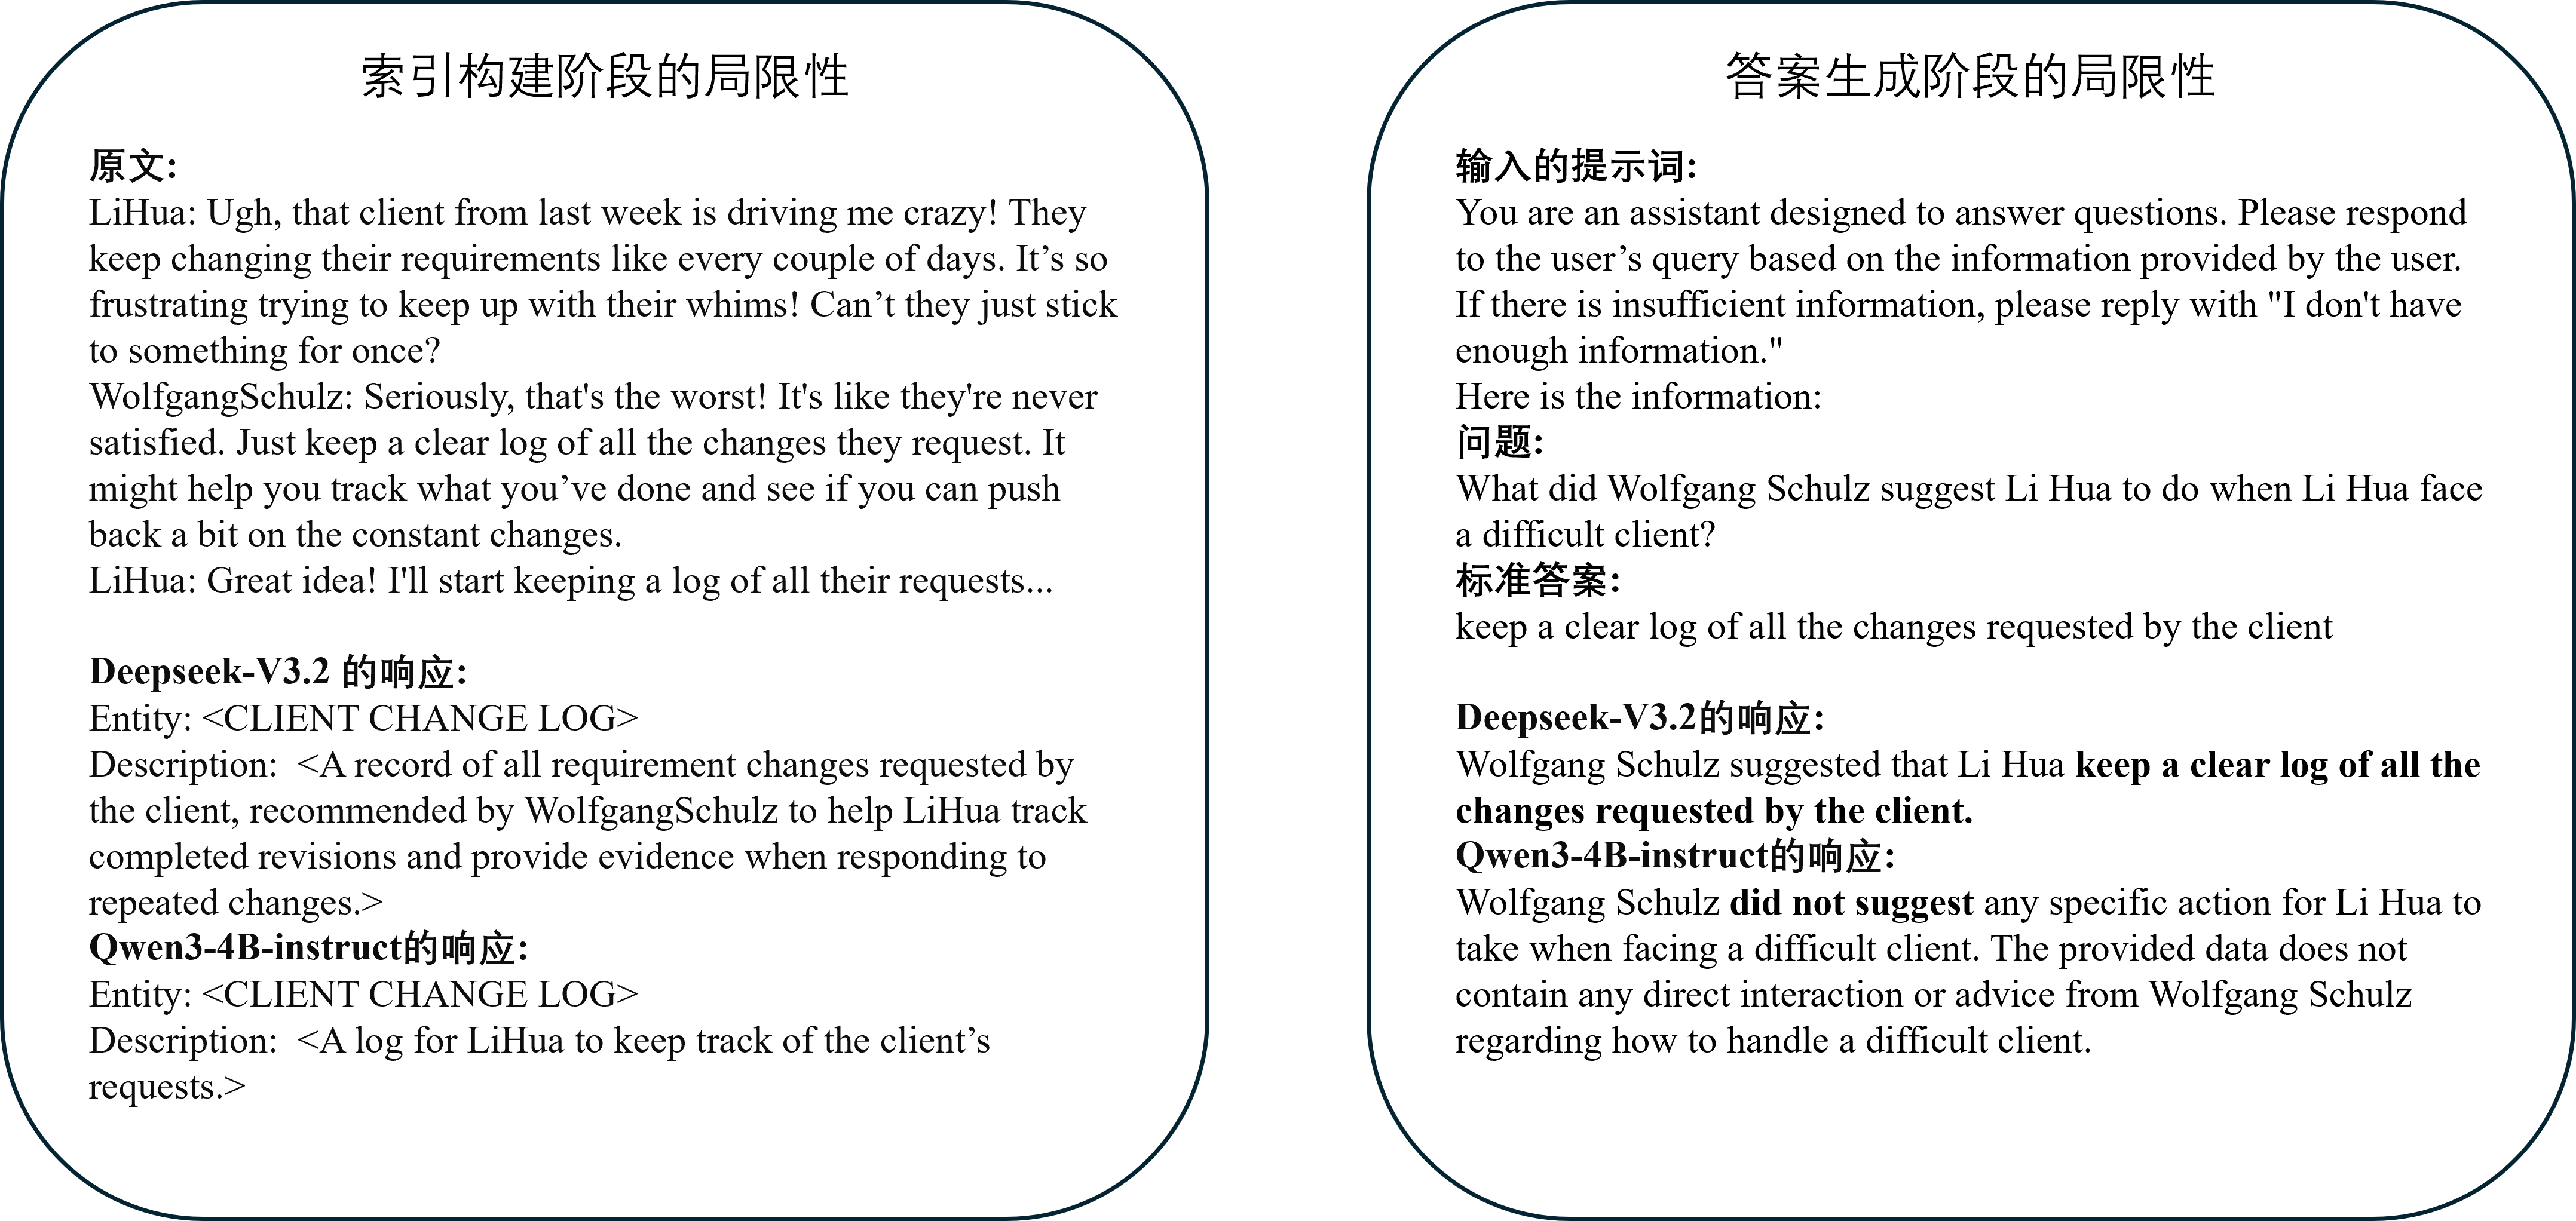
\includegraphics[width=\textwidth]{pic/3pic1.png}
\caption{SLM与LLM在图索引构建与问答中的对比示意}
    \label{fig:slmrag}
\end{figure}

如图\ref{fig:slmrag}所示,SLM(Qwen3-4B)与LLM(gpt-4o-mini)在图索引构建与问答阶段均表现出明显差异。尽管两类模型都能够识别“HOUSE RULES”这一实体,SLM生成的描述明显缺少关键细节,未能充分保留原文中所蕴含的规则信息与主旨内容。进一步地,在问答阶段,SLM较难在长上下文中稳定定位相关证据,并且更容易受到无关内容干扰,而LLM则未呈现出同等程度的性能退化。

针对上述问题,本章提出一种面向小型语言模型的验证优先图索引构建方法(Verification-First Graph Indexing Method based on SLM, VF-GIM)。如图\ref{fig:architecture}所示,该方法主要包括以下两个部分:

(1)基于验证优先的实体关系抽取模块 $E(\cdot)$。该模块基于验证优先策略,使模型在生成初始候选答案后继续执行反向验证与补全修正,从而降低SLM在开放式抽取任务中的认知负荷,并提升实体关系抽取的准确性与完整性。

(2)轻量化图数据去重模块 $D(\cdot)$。该模块在图写入阶段引入实体消歧、多源实体类型仲裁以及融合语义去重与触发式摘要的描述压缩机制,具体包括启发式实体去重、基于多数投票的实体类型决策以及基于分治策略的描述迭代摘要,从而提升图数据的纯净度并降低后续推理阶段的噪声干扰。


\begin{figure}[htb]
    \centering
    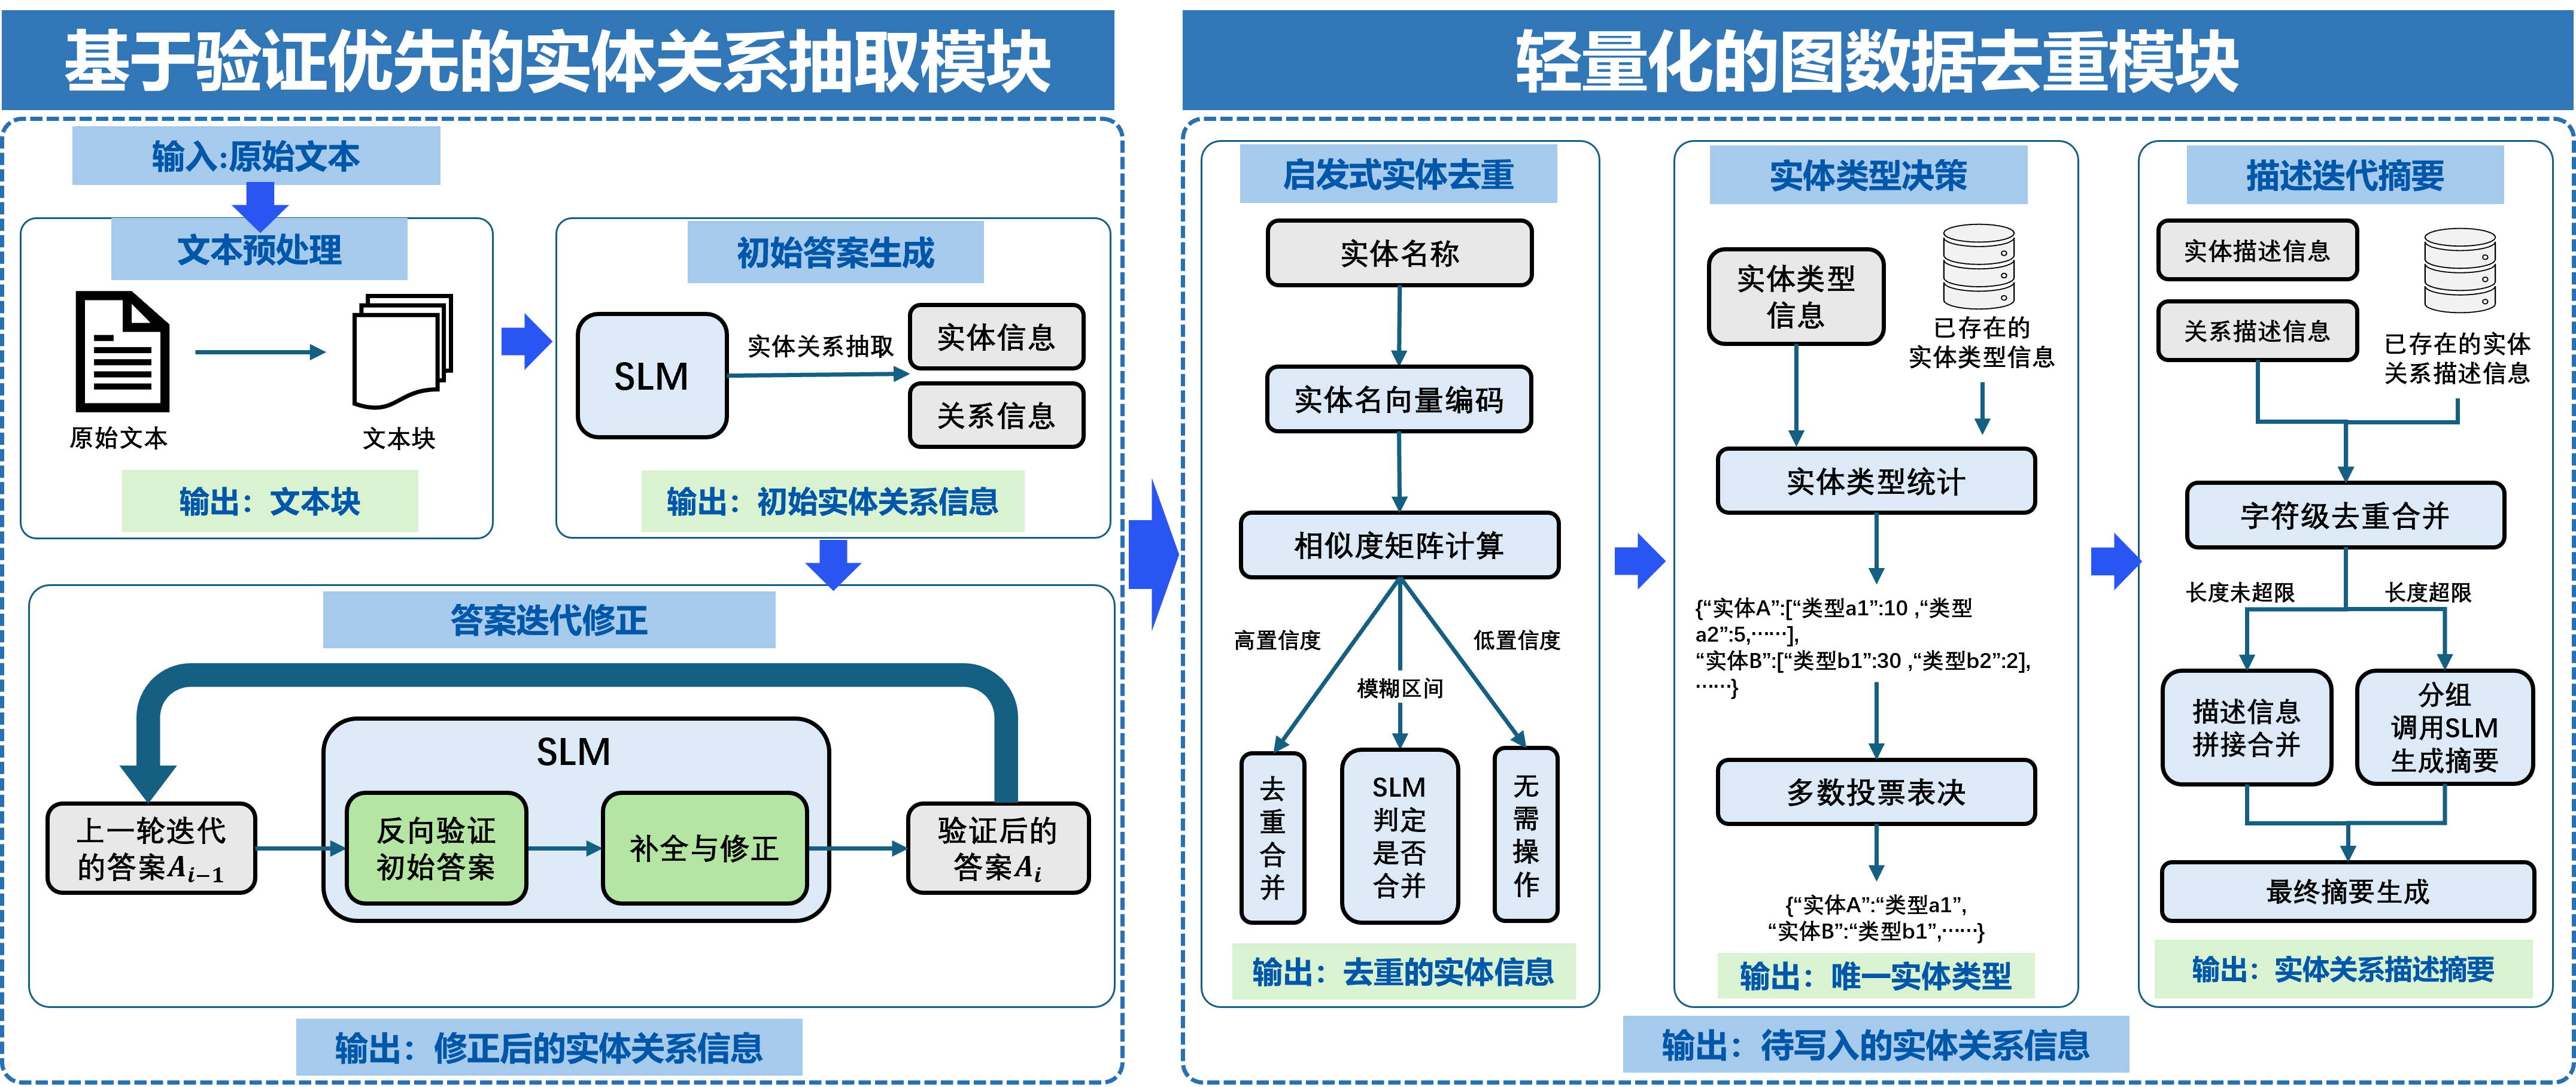
\includegraphics[width=\textwidth]{pic/3pic2.png}
\caption{图索引构建方法框架图}
    \label{fig:architecture}
\end{figure}


如表\ref{table_index_graph_comparison}所示,在相同图索引构建任务下,VF-GIM能够更有效地提升SLM对实体描述细节的保留能力,并降低检索阶段图索引中的噪声水平,从而在一定程度上缓解SLM在长上下文处理过程中的信息遗漏与幻觉问题。

\begin{table}[htb]
\centering
\caption{VF-GIM方法与现有RAG方法在图索引构建过程的优势对比}
\begin{tabular*}{\textwidth}{@{\extracolsep{\fill}}cccc}
\toprule
\multicolumn{1}{c}{对比维度}& GraphRAG  & MiniRAG  & VF-GIM   \\
\midrule
思维路径 & 正向推理 & 正向推理 & 反向验证 + 正向补全 \\
增量抽取 & 开放式提问 & 开放式提问 & 假设验证 \\
数据去重 & 字符串匹配 & 字符串匹配 & 多置信度区间消歧 \\
上下文控制 & LLM总结 & 无 & SLM总结 \\
\bottomrule
\end{tabular*}
\label{table_index_graph_comparison}
\end{table}


\section{基于验证优先的实体关系抽取模块}
传统的思维链要求模型直接从输入文本出发完成实体与关系抽取,但对于参数规模受限的 SLM 而言,这一过程往往同时包含模式识别、约束遵循与关系补全等多重认知负担,容易导致模型沿着早期错误持续生成,进而产生幻觉或遗漏。问题的关键不在于 SLM 完全缺乏抽取能力,而在于其在开放式一次生成中缺少稳定的自校正环节。
基于这一判断,本小节不再将抽取任务设计为“单轮生成尽可能完整的答案”,而是引入基于验证优先的实体关系抽取模块(Verification-First Entity-Relation Extraction, VF-ERE),将任务拆解为“先形成候选结果,再围绕候选结果进行验证与修正”的两阶段过程。其核心动机是利用“验证一个候选答案”在认知上通常比“从零生成完整答案”更容易这一特性,降低 SLM 在复杂抽取任务中的搜索难度。
验证优先策略本身是一种面向推理增强的提示范式。与标准思维链直接从问题 $Q$ 生成解题路径不同,该策略先向模型提供一个候选答案 $A'$,再要求模型在生成最终结果前对 $A'$ 的正确性进行审查。对于本章的实体关系抽取任务而言,这种设计的价值不在于增加提示复杂度,而在于改变模型的工作方式:模型不再只负责“生成”,还被显式要求承担“审计”职责,从而为小模型提供更稳定的纠错入口。其设计依据主要体现在以下两个方面:

(1)基于认知非对称性的反向推理机理。在计算复杂性理论中,验证一个已知结论的正确性通常比从零开始搜索解在认知上更简单且耗时更短。验证优先策略通过强制模型从结论回溯至前提,产生与标准正向思维链互补的逻辑信息。这种机制在处理知识密集型任务时具有显著优势,能够有效召回正向推理中易忽略的细节,并通过缩小搜索空间来提升推理精度。此外,近期的研究\cite{setlur2025scaling}指出,在测试时缩放中,若缺乏此类显式的验证环节,单纯增加生成token的数量往往无法达到最优推理性能。

(2)批判性诱导与自我中心偏差的修正。心理学研究表明,推理者在正向生成时容易陷入“自我中心偏差”,即倾向于盲目遵循自己产生的初始逻辑错误。验证优先策略通过赋予模型外部审计者的角色,要求其评价一个候选答案,从而诱发其批判性思维能力。研究\cite{alazraki2025no}发现,LLM 具备从错误中隐式学习的能力,即使初始答案是错误的,验证错误这一过程本身也能显著提升模型对逻辑结构的理解,使其比单纯的正确引导更具鲁棒性。

据此,VF-ERE 采用闭环的迭代修正机制。模型首先以标准抽取提示生成初始候选集合 $A_0$,随后在验证优先提示词的引导下对当前结果逐轮审查并修正,得到 $A_1,A_2,\dots$。这里的设计重点不是简单增加生成轮数,而是通过“保留候选结果、丢弃冗余思维历史”的方式实现测试时缩放(Test-time Scaling,TTS),使额外计算尽可能集中在纠错而非重复生成上。
这样的设计有两点直接收益。其一,与 Muennighoff\cite{muennighoff2025s1}提出的 s1 策略或传统自我修正方法\cite{madaan2023self,shinn2023reflexion}相比,本章方法在顺序迭代中仅保留上一轮的最终答案,主动切断冗余推理痕迹,从而减轻小参数模型在长上下文下的错误累积问题。其二,与 Best-of-N 等依赖并行采样和投票的策略\cite{lightman2023let}相比,验证优先策略将额外开销压缩到少量顺序迭代中,更符合 SLM 私有化部署场景下对成本与时延的约束。

VF-ERE的具体执行流程可分为以下两个阶段,如图\ref{fig:VF-ERE}所示:

\begin{figure}[htb]
    \centering
    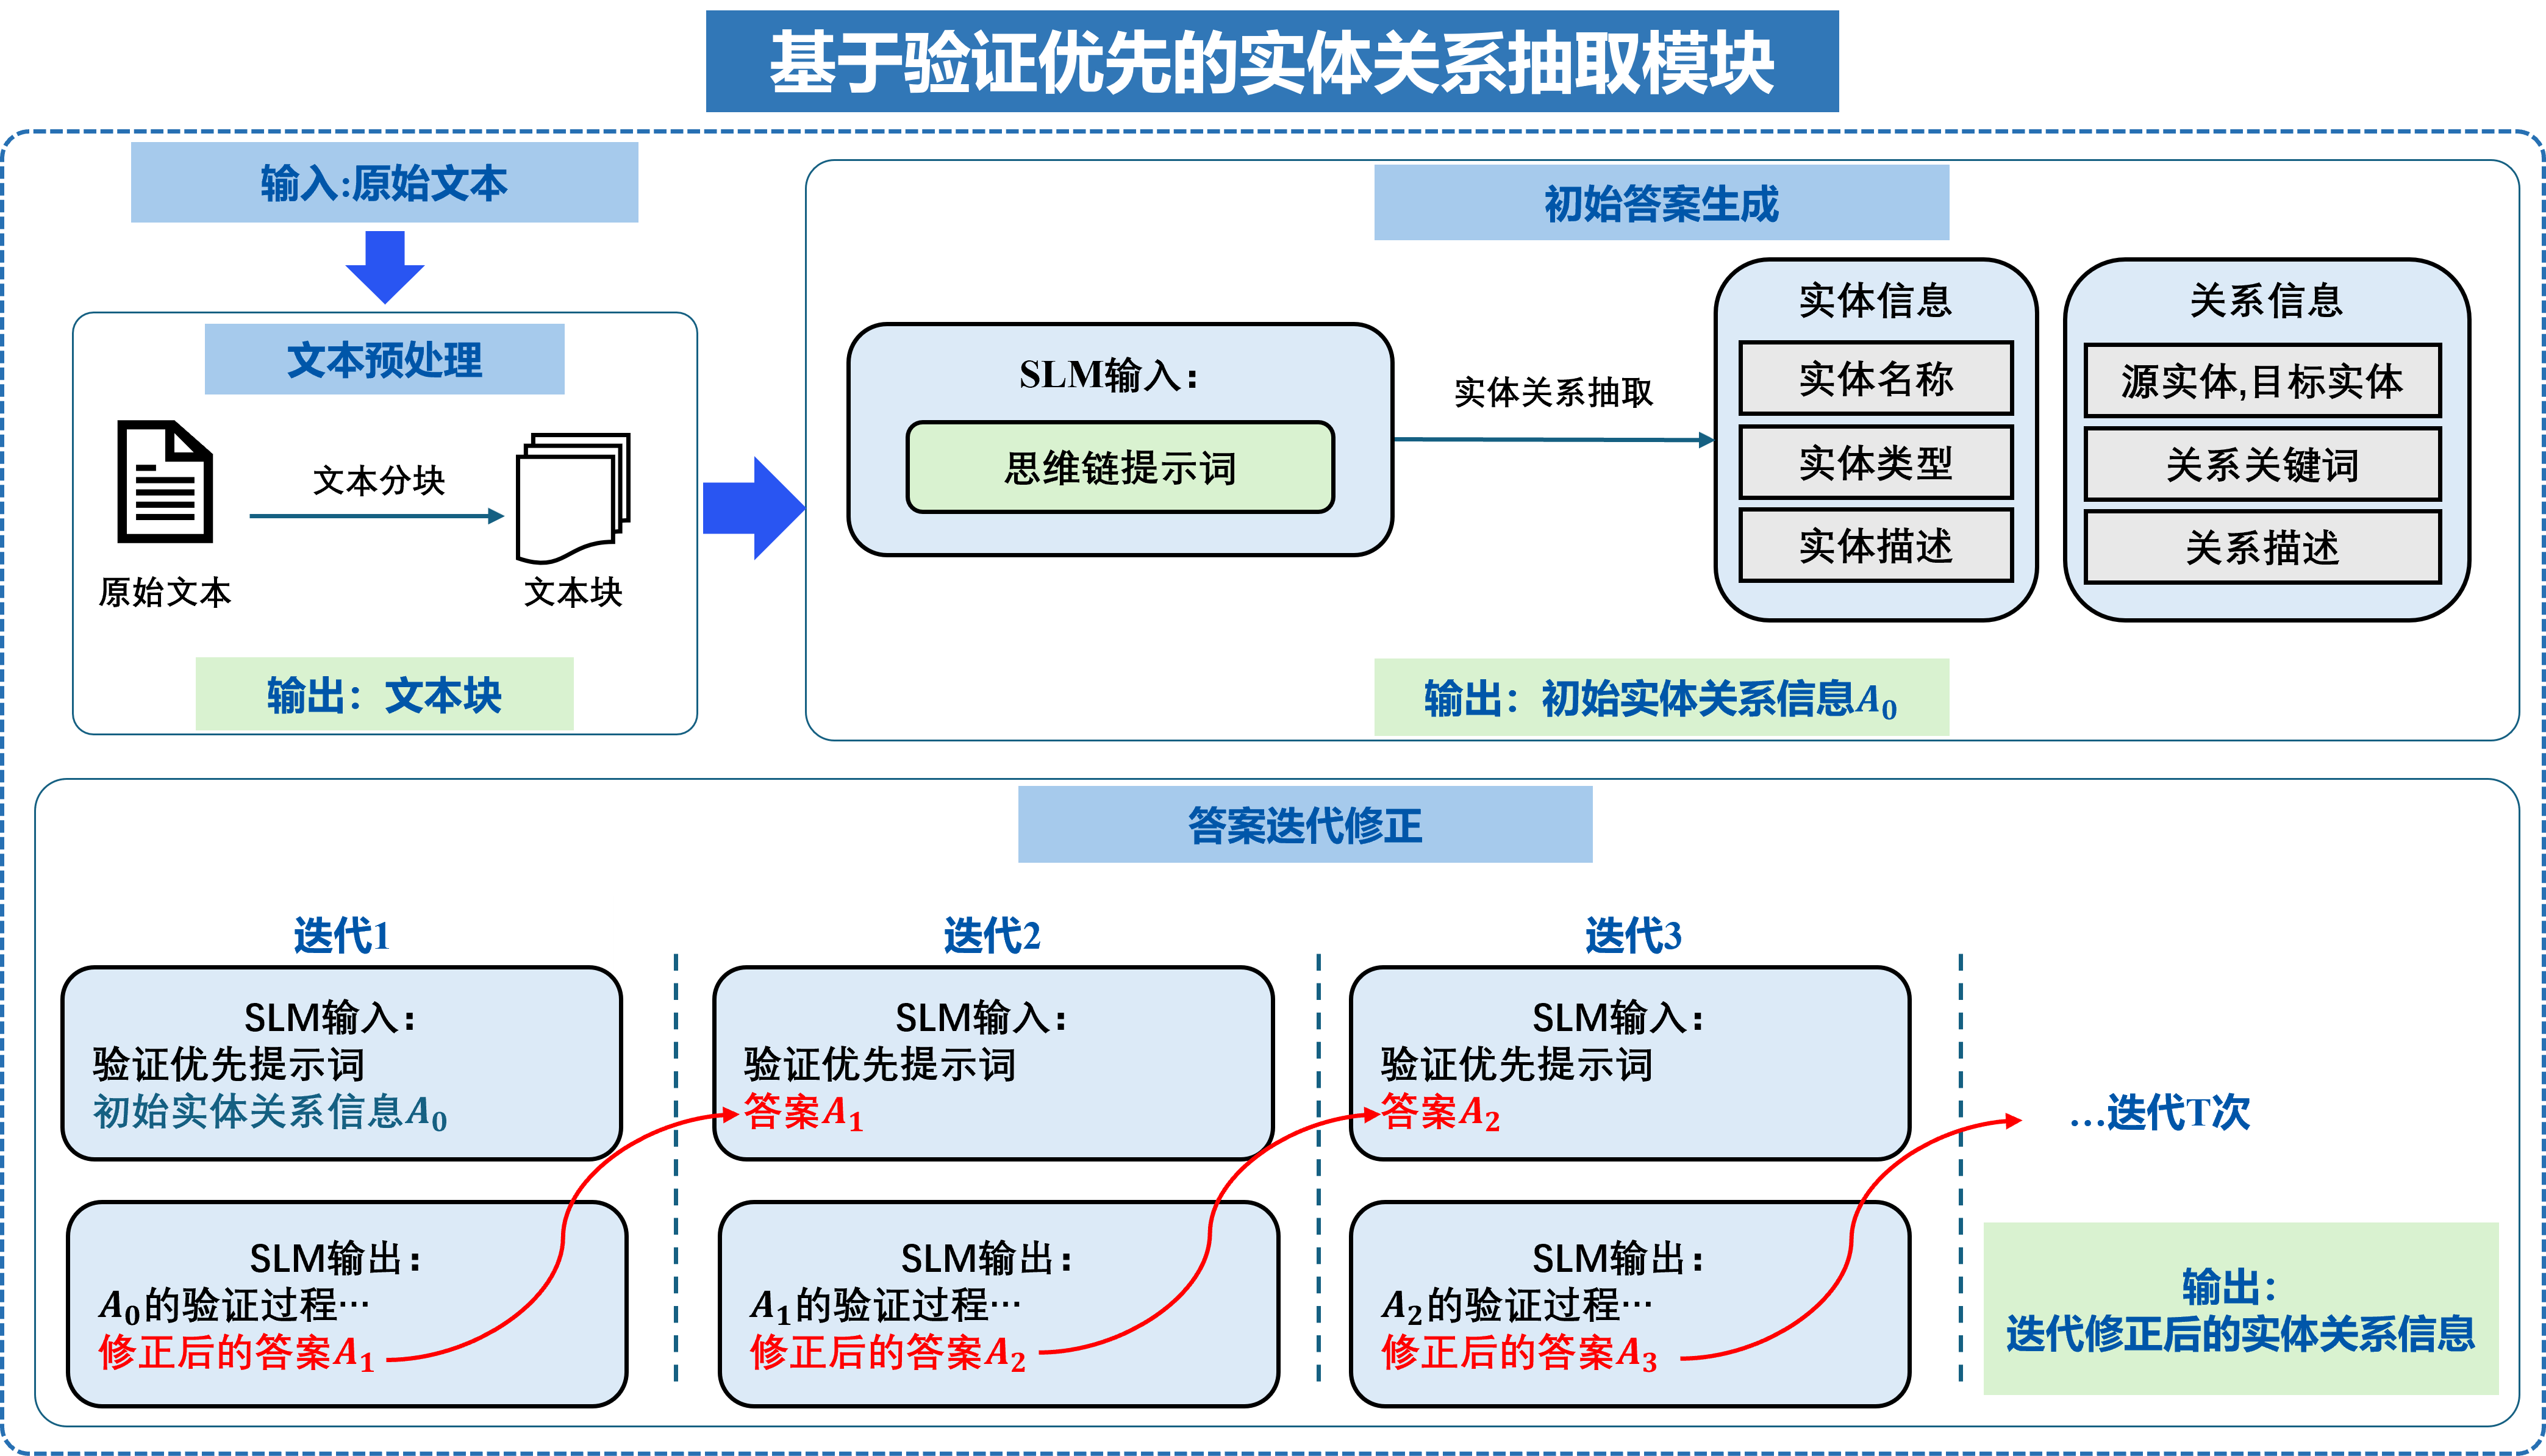
\includegraphics[width=\textwidth]{pic/VF-ERE.png}
\caption{VF-ERE流程图}
    \label{fig:VF-ERE}
\end{figure}


(1)初始答案生成阶段:输入文本$C$,构建知识图谱的实体与关系抽取任务提示词 $\tau_{0}$ ,令 SLM 生成初步的实体关系集合 $A_0$。
这一阶段的目标不是一次性得到完全准确的最终结果,而是尽可能生成结构完整、便于后续审查的候选抽取结果。因此,提示词 $\tau_{0}$ 的设计重点在于先约束输出边界,再尽量提高候选结果的可验证性。如图\ref{fig:prompt_initial}所示,其主要考虑如下:

首先,明确要求首先识别实体。为每个识别到的实体提取实体特征信息,信息包括实体名称、实体类型及实体语义描述。其中,实体的名称要求和原文使用相同的语言;实体类型需来自预定义的Schema列表,以约束模型的识别范围,减少无关实体的干扰。实体语义描述要求是对实体属性与活动的全面描述。

其次,在已识别实体集合上,令模型识别满足“明确相关性”阈值的实体对,并提取关系特征信息, 信息包括源实体名称、目标实体名称、关系关键词及关系语义描述。通过先行锚定实体,减少了模型在抽取关系时的幻觉风险。

然后,基于小样本学习的思想,在提示词中提供三个覆盖不同情境的示例,示例展示了实体类型的约束作用,教导模型仅关注特定Schema下的信息,抑制模型输出无关实体的倾向。

最后,在输出格式的设计上,提示词采用自定义的分隔符替代JSON格式输出,能够显著减少Token的消耗,提高推理效率。

\begin{figure}[htb]
    \centering
    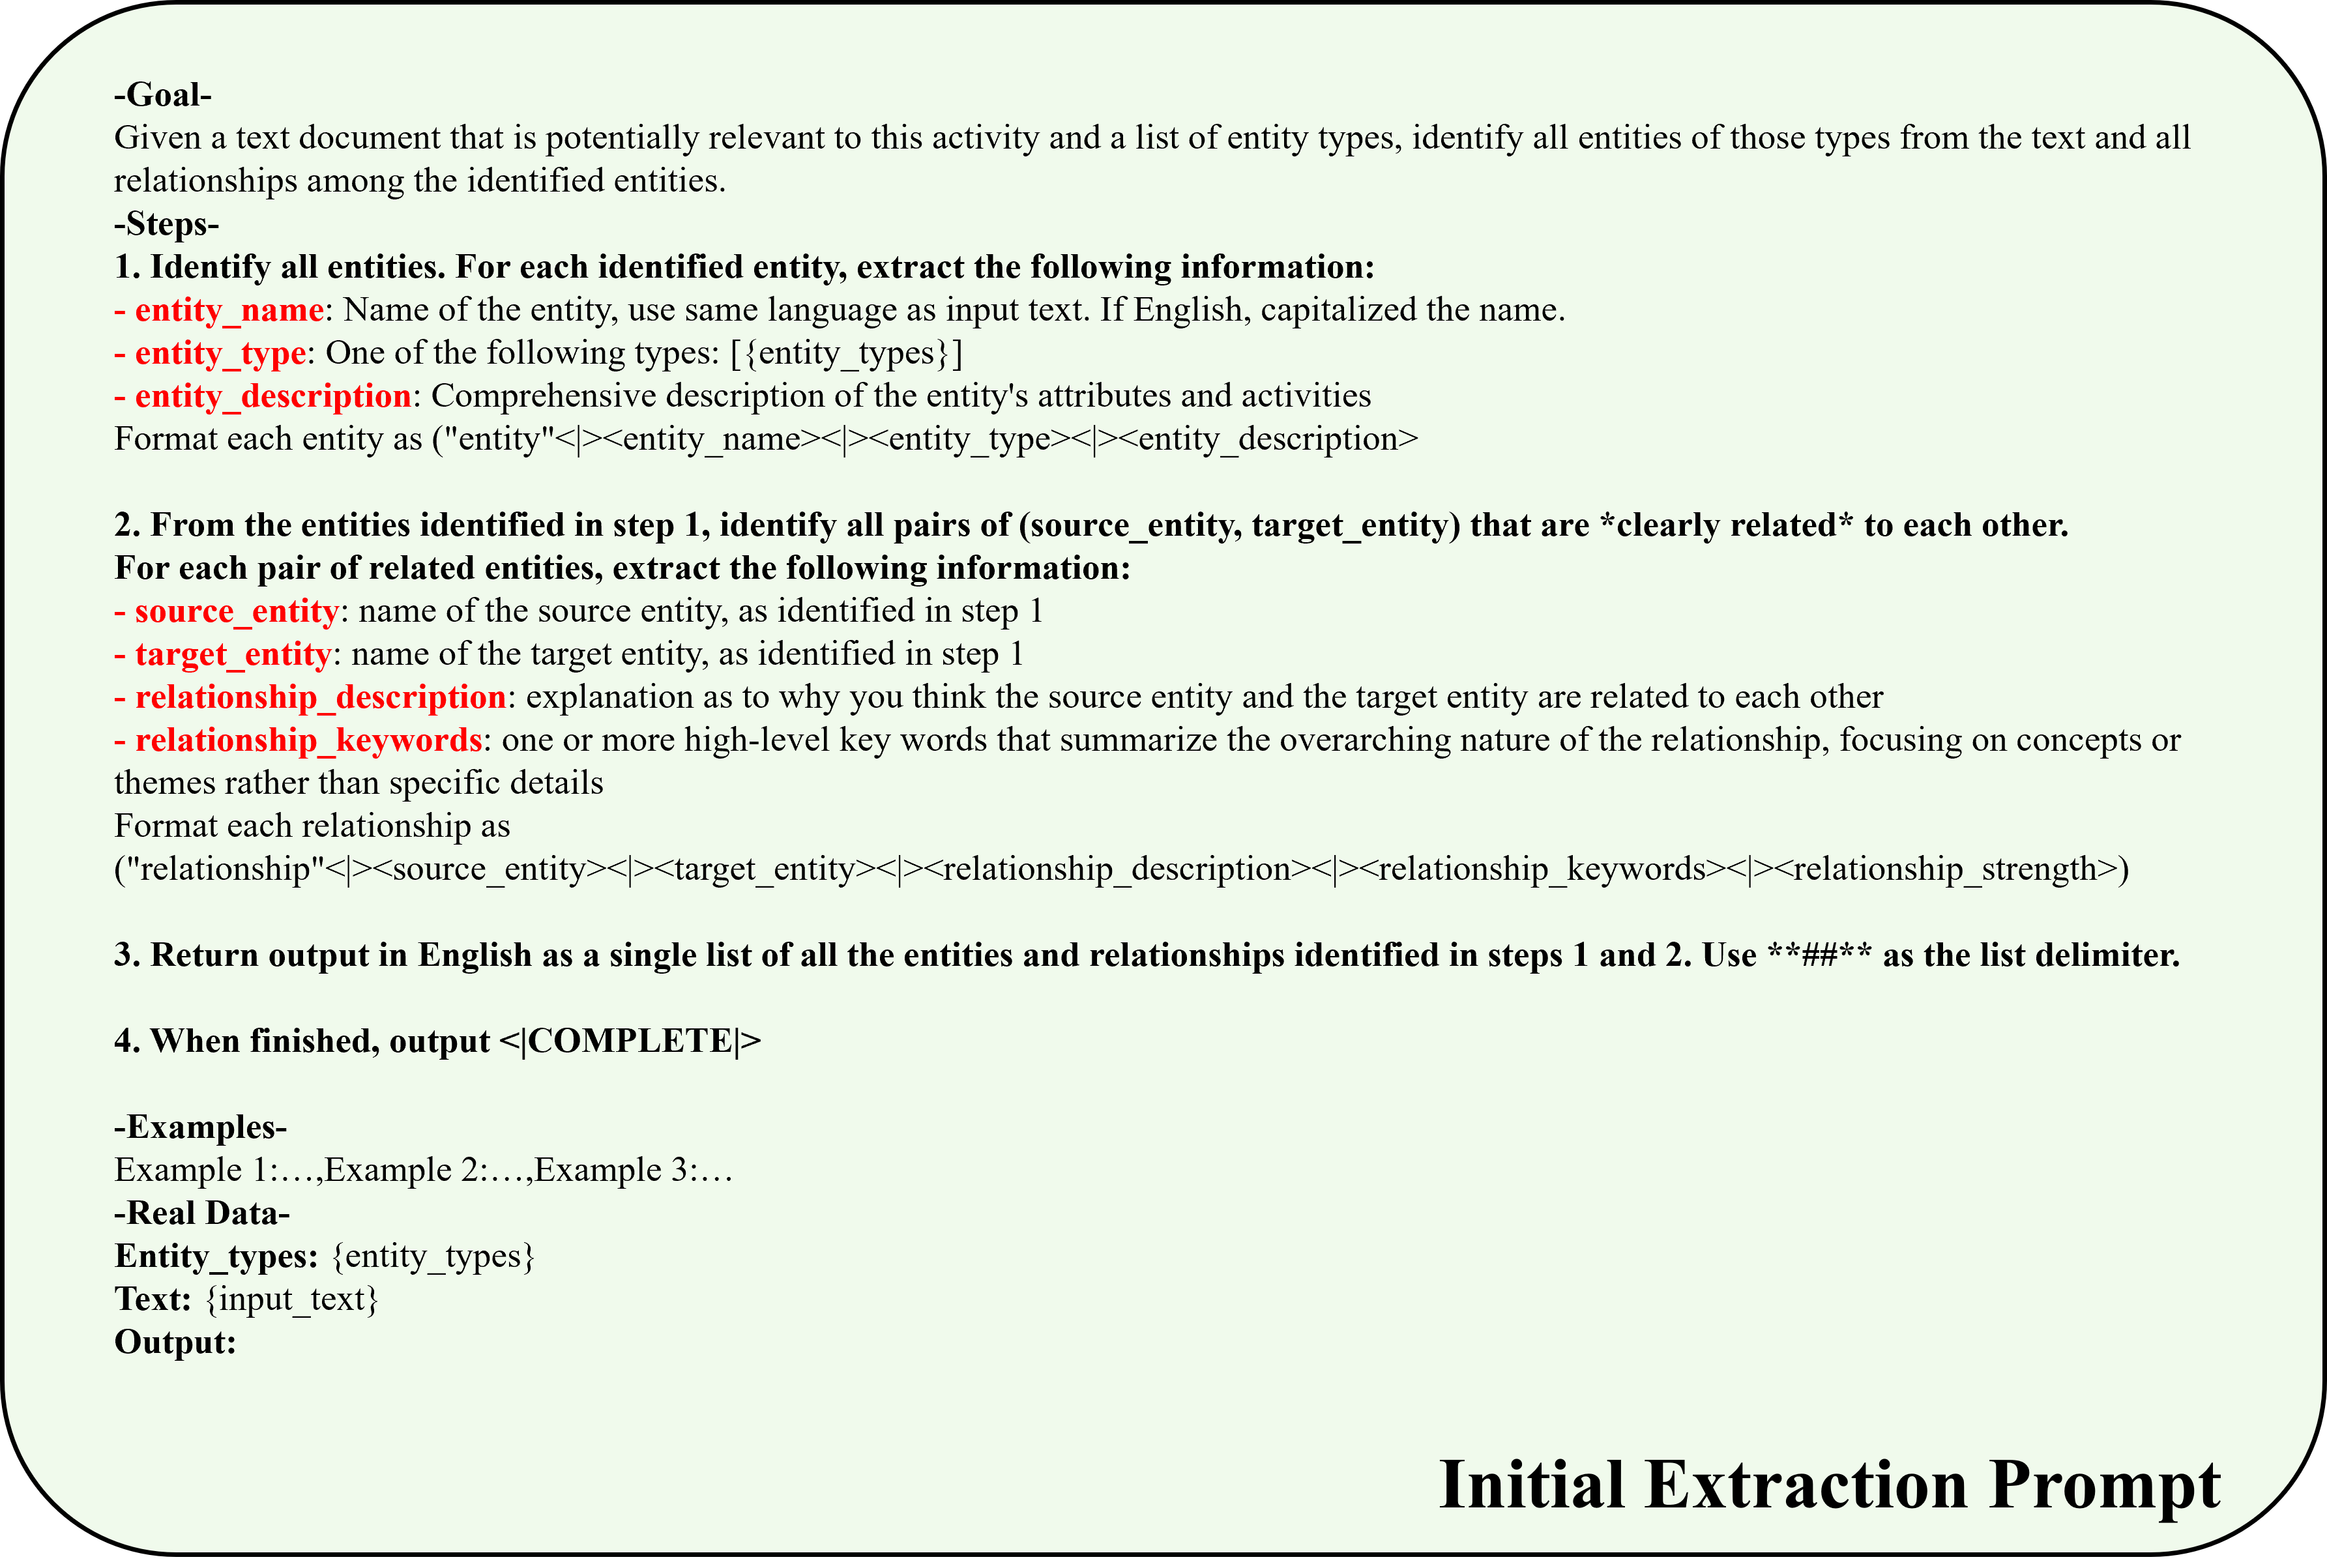
\includegraphics[width=\textwidth]{pic/initial_extract.png}
\caption{实体关系抽取初始提示词模板}
    \label{fig:prompt_initial}
\end{figure}

(2)迭代修正阶段:在迭代过程中,模型根据验证优先提示词 $\tau_{vf}$ 对当前的候选实体关系集合 $A_{i-1}$ 进行修正。与初始阶段相比,这一阶段的核心任务已经从“尽量抽取”转向“定位缺失与错误并完成补正”,其目的在于利用测试时缩放提升小型模型在复杂语义提取任务中的鲁棒性。提示词$\tau_{vf}$如图\ref{fig:prompt_VF}所示。

\begin{figure}[htb]
    \centering
    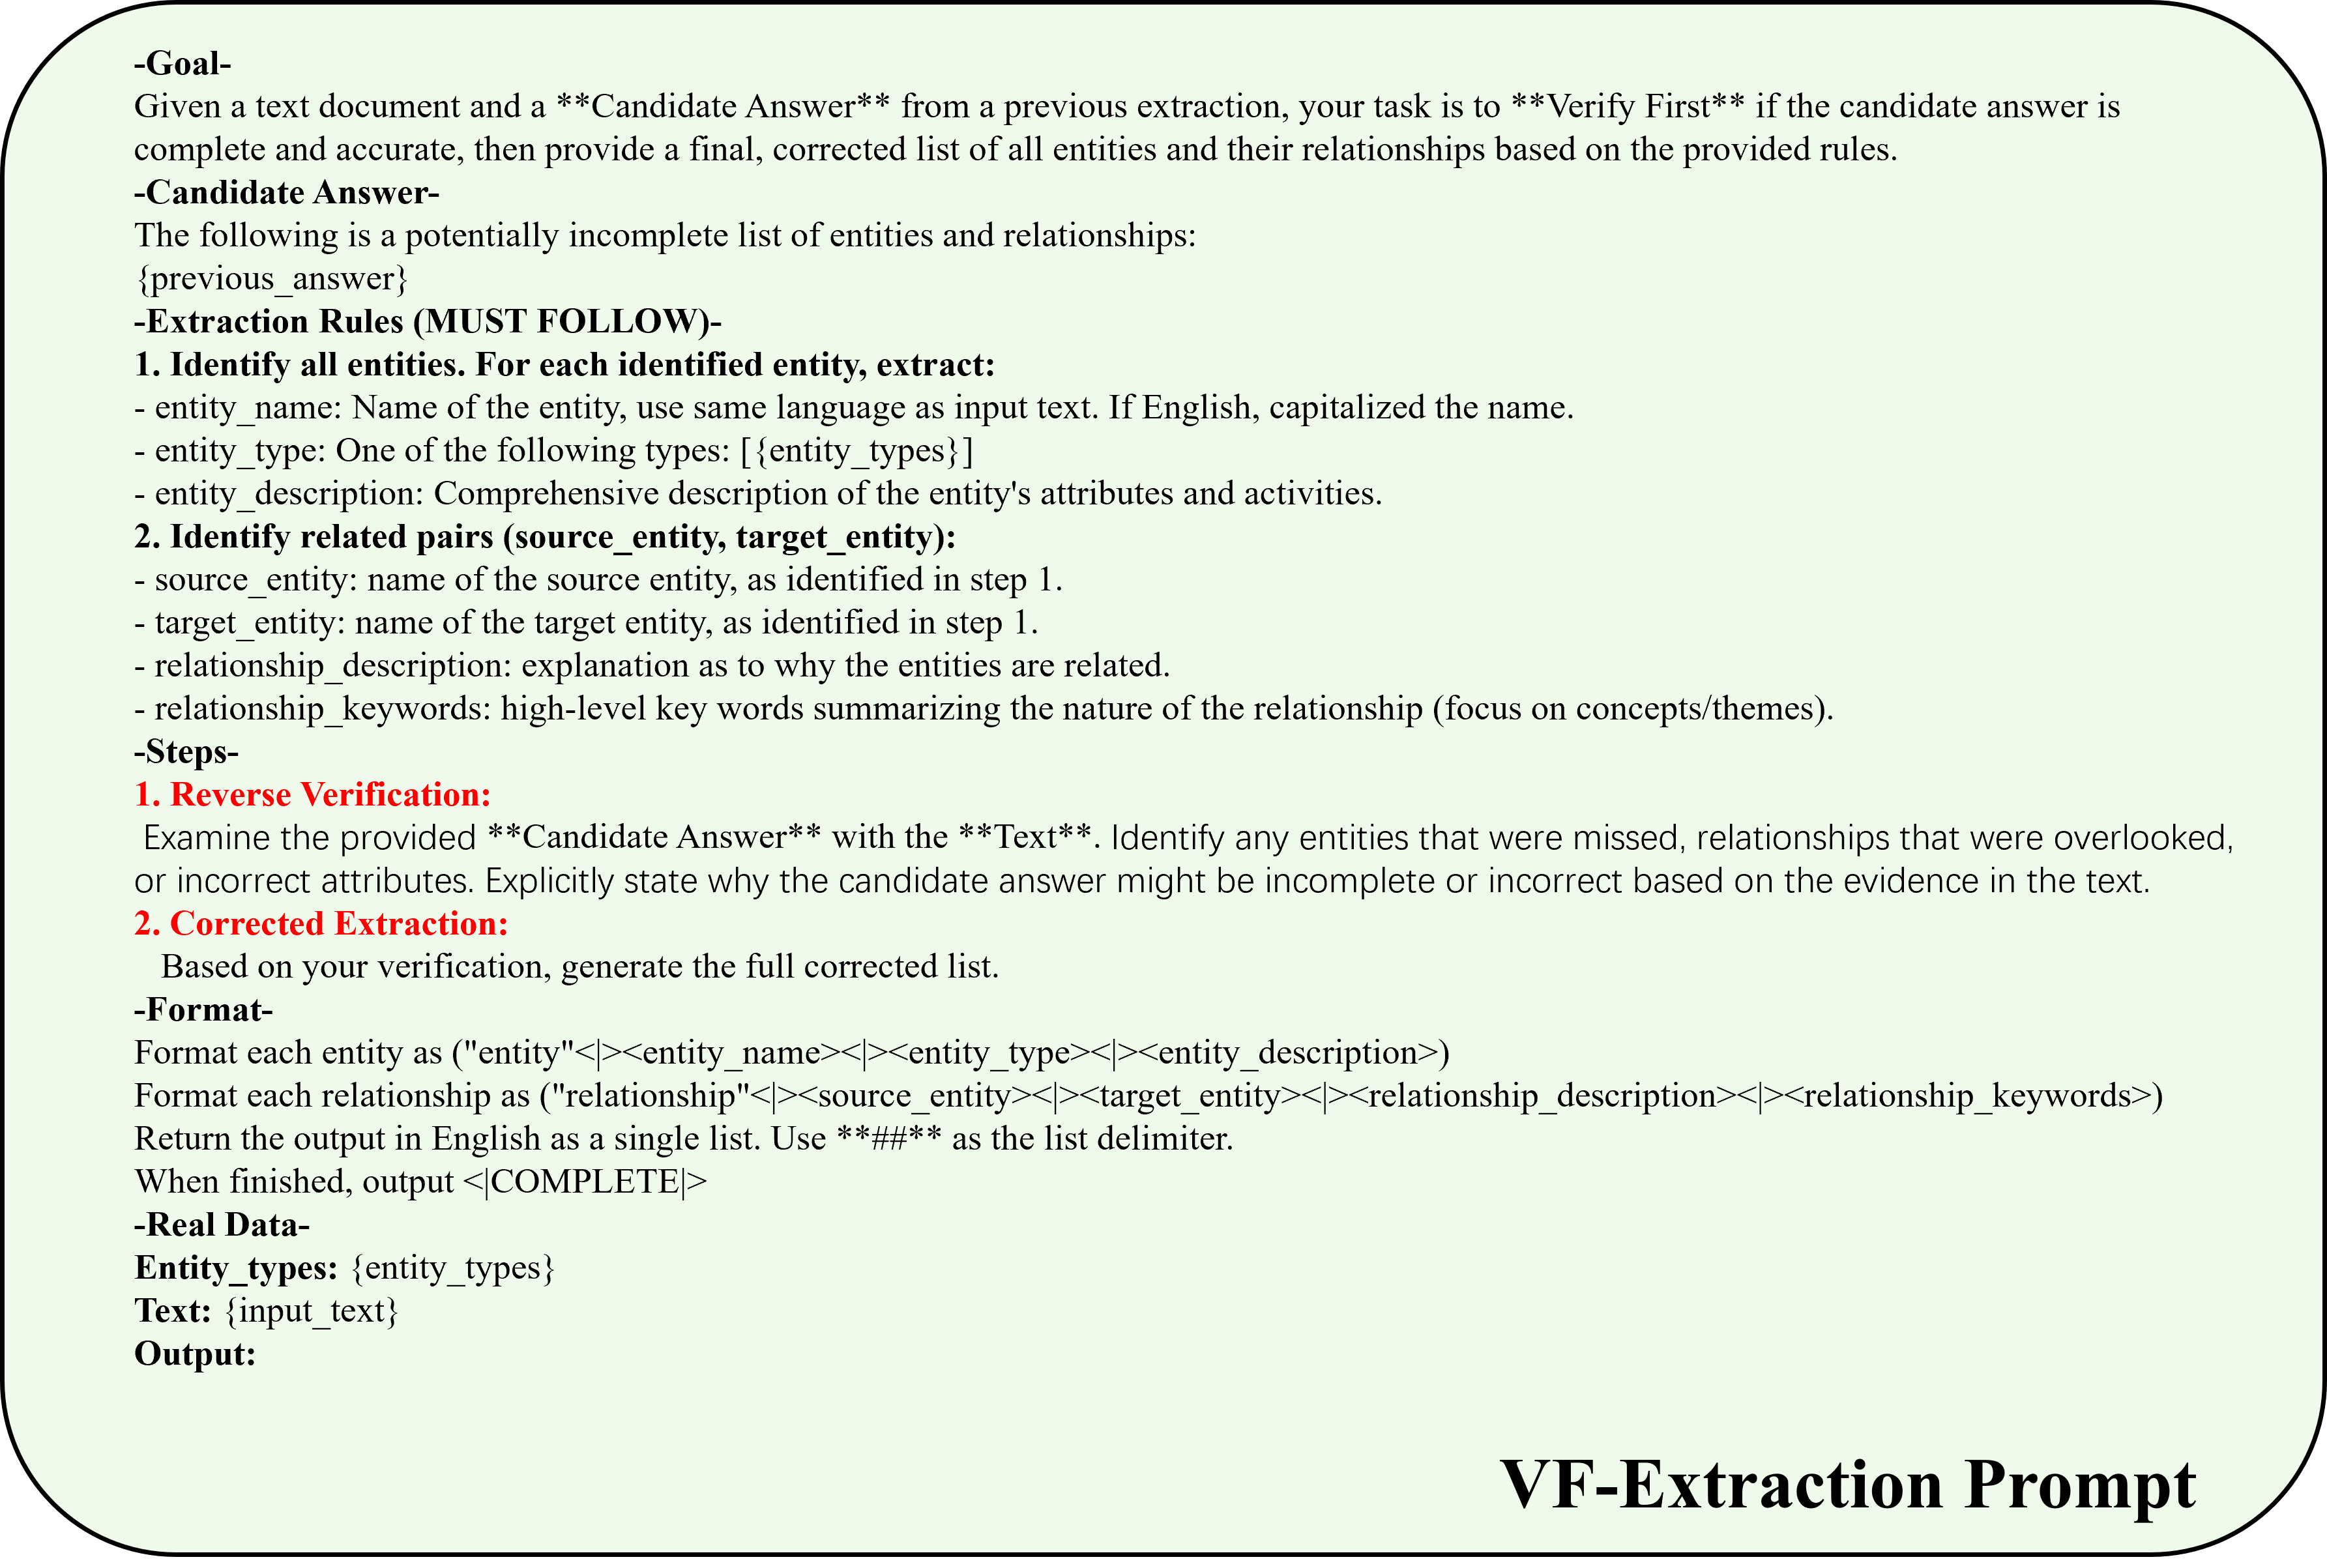
\includegraphics[width=\textwidth]{pic/VF_prompt.png}
\caption{实体关系抽取迭代提示词模板}
    \label{fig:prompt_VF}
\end{figure}

提示词 $\tau_{vf}$ 的设计遵循“验证优先”策略,其重点不在于延长思维链,而在于让模型围绕“当前答案哪里不对、还缺什么”开展针对性审查。具体设计逻辑包括以下核心维度:

在执行验证-修正指令前,系统将上一轮输出的提取结果 $A_{i-1}$ 作为本轮迭代的候选答案提供给模型。
首先,提示词设计中特意去除了上一轮的推理路径,仅保留最终生成的实体关系列表。这种设计赋予了迭代过程马尔可夫特性,能够有效避免长序列生成中常见的上下文溢出以及由先前逻辑谬误导致的错误累积效应。

其次,考虑到小型语言模型在指令遵循及隐含知识检索方面的局限性,提示词在每一轮迭代中均嵌入了完整的实体关系抽取规则。显式的属性解释,如实体类型的范围,为模型提供了客观的判别准则。若缺失规则细节,4B及以下参数规模的小型语言模型将难以准确评判候选答案中的描述是否满足“完整性”要求,进而可能导致输出质量退化,增加逻辑错误的风险。

在执行验证-修正时,首先进行反向验证。模型将提供的候选答案与原始文本进行对比。这一步骤的核心在于触发模型的反向推理过程,在认知层面上反向推理比标准的正向思维链推理更具启发性,并且负担更轻。通过识别候选答案中遗漏的实体或错误的关系,模型能够克服自回归生成中常见的“自我中心偏差”,即盲目遵循先前错误生成路径的倾向。此过程缩小了模型的搜索空间,并为后续生成提供了互补的信息支撑。

在完成反向验证的分析后,模型进入最终的生成环节。在验证阶段的基础上,模型需整合验证阶段发现的逻辑漏洞,并利用已建立的反向推理路径作为引导,生成修正后的实体关系列表。该步骤要求模型将正确信息与修正信息进行融合重构,从而在不增加训练成本的前提下,有效降低复杂关联提取中的逻辑失误率。

迭代修正阶段中,第 $i$ 次迭代中,得到$A_i$的过程如下:
$$A_i = \text{SLM}(C, A_{i-1}, \tau_{vf}), \quad 1 \le i \le T$$

其中,$C$为输入文本,$T$ 为预设的最大迭代轮数。初始轮首先生成 $A_0$,随后模型在验证优先提示词 $\tau_{vf}$ 的引导下迭代生成 $A_1,\dots,A_T$ 中的候选结果,直至满足终止条件。

算法在满足预设条件时终止:一是迭代次数达到预设的阈值$T$(通常设定为2-3次);二是模型回答中确认上一个答案$A_{i-1}$已完全覆盖文本$C$中的所有信息。最终,将最后一个轮次的答案作为最终的实体关系集合。

上述模块将复杂的实体关系抽取转化为一个“验证-修正”的循环过程,使模型在不增加训练成本的前提下,利用额外的测试时间计算换取更高的推理质量。

\section{轻量化的图数据去重合并模块}
若前一小节解决的是“如何尽可能正确地抽取实体关系”,那么本节面对的问题则是“如何在持续写入过程中避免图索引被冗余与冲突信息拖垮”。在多文档或长文档场景下,同一实体或关系往往会反复出现在不同文本块中;如果写入阶段仍采用字符级去重与直接拼接的策略,则前端抽取质量即使有所提升,也会在后续合并过程中被重复节点、类型漂移和超长描述重新稀释。现有 SLM 驱动的图基检索增强生成系统大多仅通过集合去除完全重复的字符串后进行物理拼接,这一处理方式至少带来以下两个问题:

(1)上下文膨胀与语义冗余:由于缺乏基于语言模型的语义压缩,高频实体与关系的描述字段会无限增长,且充斥着语义重复但表述略异的文本。以 MiniRAG 一类未引入描述摘要机制的系统为例,历史描述在增量写入阶段往往会被持续直接拼接,这不仅浪费了存储空间,更会在最终问答阶段占据大量上下文窗口,使其他关键证据被超长实体或关系描述淹没。

(2)缺乏实体对齐与冲突解决:依赖严格的字符串匹配导致了实体对齐功能的缺失,且简单的文本拼接无法解决逻辑冲突,导致图谱中可能残留自相矛盾的信息。

基于上述观察,本节将图写入优化拆分为三个互补问题:实体是否应该合并、合并后类型如何确定、累积描述如何压缩。围绕这三个问题,本文设计轻量化的图数据去重合并模块,分别对应启发式实体去重、基于多数投票的实体类型决策以及基于分治策略的描述迭代摘要。这样的拆分并非模块堆叠,而是因为三类错误的来源不同:前者主要影响图中节点冗余,中者影响知识表示的一致性,后者则直接决定后续检索时的上下文负担。


实体去重的核心矛盾在于,如果完全依赖字符串匹配,别名、简称与跨文档表述差异会造成大量重复节点;但如果对所有候选实体对都调用语言模型进行语义判别,写入成本又会迅速上升。基于这一权衡,本文采用启发式实体去重机制:先用轻量嵌入模型完成大范围筛选,仅在向量相似度落入模糊区间时调用 SLM 进行二次仲裁。这样做的动机是将大模型判断能力留给真正边界不清的样本,而把明显可分或明显可并的情况交给低成本规则处理。该方法将传统字符级去重提升到语义维度,具体形式化描述如下:

首先,在图索引的增量更新阶段,设当前待处理的实体集合为 $\mathcal{E}_{batch} = \{e_1, e_2, \dots, e_n\}$。模块首先利用轻量化语义嵌入模型 $\phi(\cdot)$ 对每个实体的标识符,即实体名称进行映射,得到其在高维空间中的稠密向量表示:
$$\mathbf{h}_{i} = \phi(\text{name}(e_i)), \quad \mathbf{h}_{i} \in \mathbb{R}^d$$

随后,通过计算$\mathcal{E}_{batch}$中两两实体间的余弦相似度,构建相似度矩阵 $\mathbf{S} \in \mathbb{R}^{n \times n}$,其中矩阵元素 $s_{ij}$ 定义为:
$$s_{ij} = \cos(\mathbf{h}_i, \mathbf{h}_j) = \frac{\mathbf{h}_i^\top \mathbf{h}_j}{\|\mathbf{h}_i\| \|\mathbf{h}_j\|}$$

算法根据相似度评分 $s_{ij}$ 所处的区间,采取差异化的实体对齐策略以平衡计算效率与判定精度:

低相关度独立区间 ($s_{ij} \le \tau_{low}$):若 $s_{ij}$ 低于下限阈值 $\tau_{low}$(例如 0.82),则判定两实体在语义层面具有显著差异,视为独立节点存入图索引 $\hat{\mathcal{D}}$ ,不触发合并操作。

逻辑高置信度合并区间 ($s_{ij} > \tau_{high}$):若 $s_{ij}$ 超过上限阈值 $\tau_{high}$(例如 0.91),则算法以极高置信度判定 $e_i$ 与 $e_j$ 为同一语义实体。系统将触发合并流程。

语义模糊判定区间 ($\tau_{low} < s_{ij} \le \tau_{high}$):当相似度处于模糊区间(0.82 至 0.91)时,单纯依靠向量距离难以区分语义近义词与具体差异。此时,引入额外的SLM作为二次仲裁算子,对候选实体对执行共指判定:
$$\text{Decision} = \text{SLM}(\text{Profile}(e_i), \text{Profile}(e_j))$$

具体而言,系统将两个实体的完整属性,包括名称、类型与描述信息组织为输入,要求模型判断实体 A 与实体 B 是否指向同一真实世界对象。具体模型本文选用Qwen3-0.6B,该模型主打低成本、高推理速度与强语义理解能力。
与开放式生成任务不同,该步骤被约束为一个保守的判别任务,其核心目标不是尽可能促成合并,而是在语义边界不清晰的情况下尽量避免误合并对图结构造成不可逆污染。
为此,本文在提示设计中显式采用保守决策原则,如图\ref{fig:prompt_merge}所示：
\begin{figure}[htb]
    \centering
    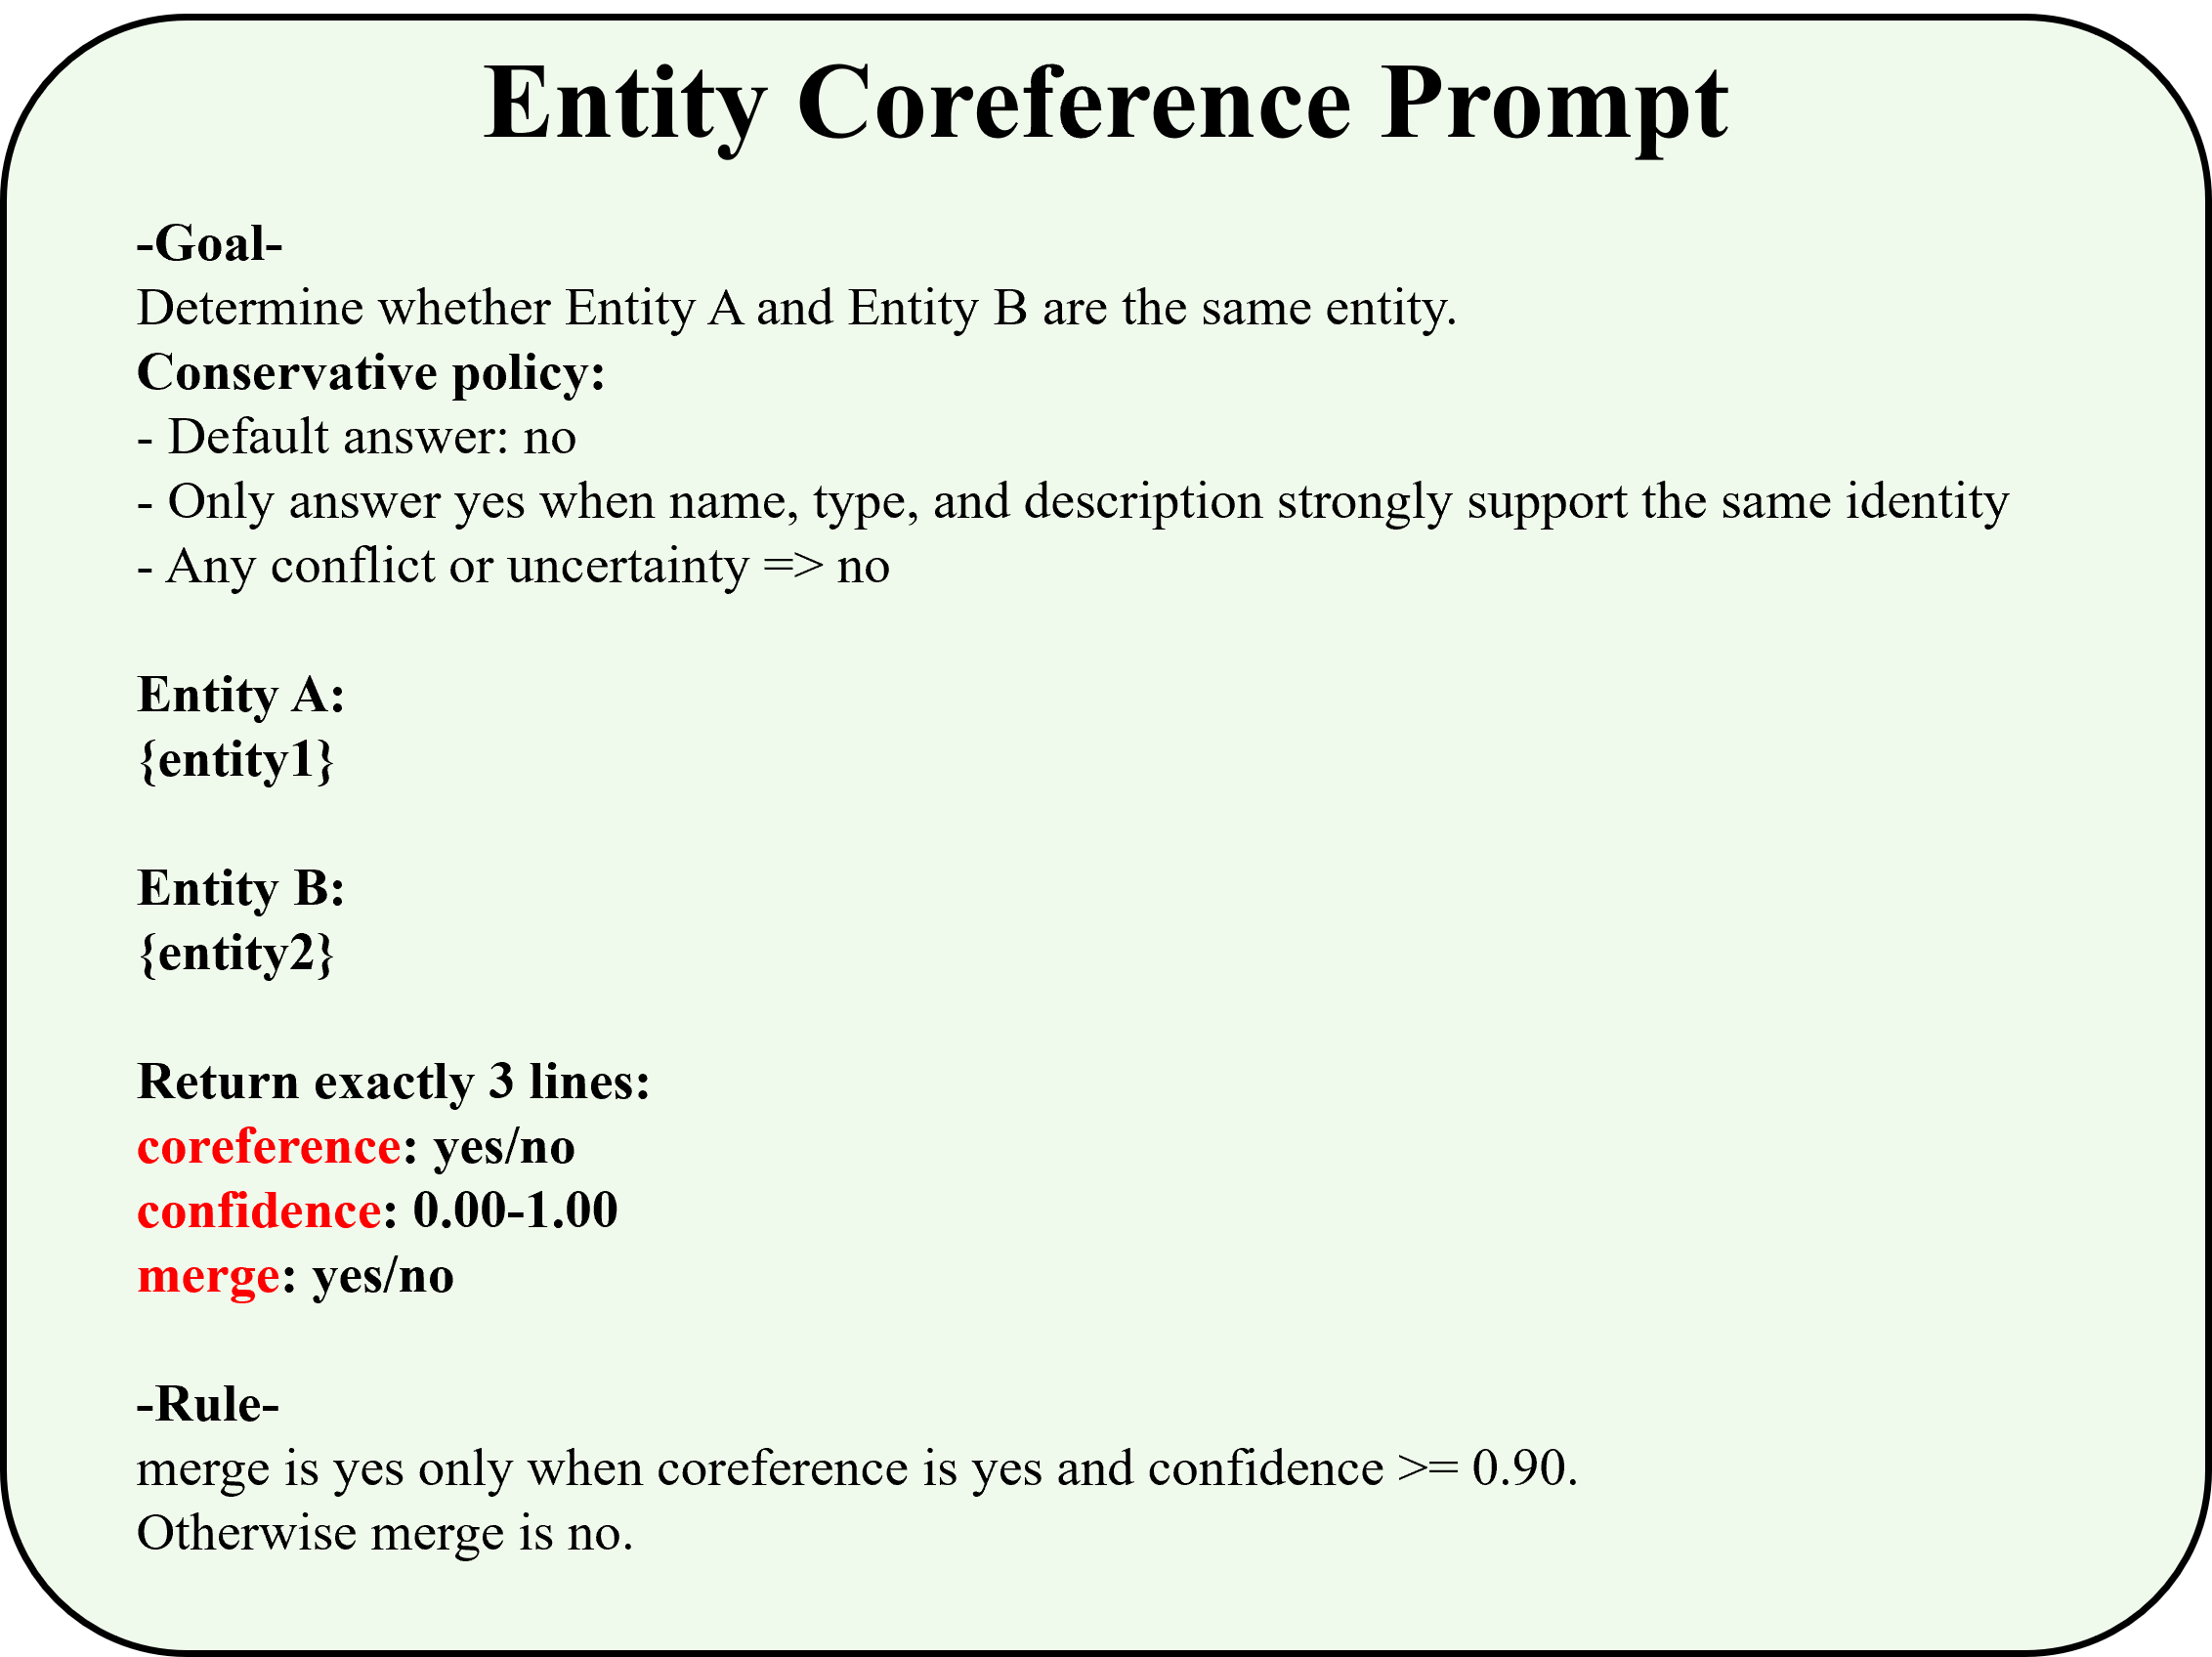
\includegraphics[width=0.8\textwidth]{pic/3pic_merge_prompt.png}
\caption{启发式实体去重提示词模板}
    \label{fig:prompt_merge}
\end{figure}

模型默认输出“不共指”,只有当两个实体在名称层面具有高度对应关系、在类型层面保持一致,且描述中的核心属性、关系或事件信息能够相互支持而不存在明显冲突时,才允许输出“共指”。
若存在名称仅部分相似、实体类型不一致、描述中出现时间或身份冲突、关键信息不足,或模型无法形成高置信判断等情形,则统一判定为“不共指”。

在输出形式上,模型返回 coreference、confidence 与 merge 三项结果,其中 coreference 表示是否共指,confidence 表示判定置信度,merge 表示是否触发实体合并。为进一步提高图写入过程的稳健性,系统仅当 coreference = yes 且 $confidence \ge 0.90$ 时才执行合并；其余情况均保留为独立节点写入图索引。

上述设计使得模糊区间内的实体消歧从单纯的向量近邻判断扩展为结合名称、类型与描述的属性一致性判别过程。一方面,该机制避免了对所有实体对统一调用语言模型所带来的额外开销,保持了索引构建阶段的效率可控；另一方面,又能够在别名、简称、跨文档表述差异以及局部信息不完整等场景下提供比字符串匹配更强的语义对齐能力,从而降低重复实体率,提升图索引的纯净度与一致性。


在跨文档的实体提取过程中,由于SLM对同一实体在不同语境下的理解偏好存在差异,往往会导致提取的实体类型出现不一致性。为了增强知识图谱的分类一致性并防止历史知识被错误覆盖 ,本研究在去重模块 $D(\cdot)$ 中引入了一种基于多数投票的实体类型决策机制,算法流程如图\ref{alg:vote}所示。该机制的具体形式化描述如下:

(1)类型集合的聚合:对于给定实体 $e_i$,设当前提取批次产生的候选类型集合为 $\mathcal{T}_{new} = \{\tau_1, \tau_2, \dots, \tau_n\}$。
若该实体已存在于全局知识图谱 $\hat{\mathcal{D}}$ 中,系统将首先检索其已存储的历史类型 $\tau_{hist}$,并将其并入实体类型集合$M$ 中:
$$M = \mathcal{T}_{new} \uplus \{\tau_{hist}\}$$

这一过程确保了在增量更新过程中,历史累积的分类证据具有与新提取信息同等的权重,从而实现了对既有知识的保护。


(2)多数投票决策:最终实体类型 $T^*$ 的决策逻辑建立在频次极大化原则的基础上。系统对 $M$ 中的各类标签进行频率计数,选择频率最高的类型作为实体的规范化标签:
$$T^* = \text{arg}\max_{\tau \in \text{unique}(M)} \text{freq}(\tau, M)$$

通过该机制,系统能够有效滤除SLM在单次提取中产生的偶然性噪声。例如,若某实体在历史记录中被标记为“地点”,而在当前批次中出现了一次的“公司”标签,但同时伴随三次“地点”标签,系统将依据频率优势锁定其类型为“地点”。

\begin{algorithm}[h]
    \SetAlgoLined
\caption{多数投票实体类型决策}
    \label{alg:vote}
    \KwData{实体 $e_i$,当前提取批次产生的候选类型集合 $\mathcal{T}_{new} = \{\tau_1, \tau_2, \dots, \tau_n\}$, 全局知识图谱 $\hat{\mathcal{D}}$}
    \KwResult{最终实体类型 $T^*$}

    初始化实体类型集合 $M \gets \emptyset$\;
    \If{$e_i \in \hat{\mathcal{D}}$}{
        检索历史类型 $\tau_{hist} \gets \text{GetNodeType}(\hat{\mathcal{D}}, e_i)$\;
        $M \gets M \uplus \{\tau_{hist}\}$ \tcp*{将历史知识存入实体类型集合以保护既有证据}
    }
    \For{每个候选类型 $\tau_i \in \mathcal{T}_{new}$}{
        $M \gets M \uplus \{\tau_i\}$ \tcp*{聚合当前批次的观测数据}
    }
    $T^* \gets \arg \max_{\tau \in \mathrm{unique}(M)} \mathrm{freq}(\tau, M)$\;

    \Return $T^*$\;
\end{algorithm}


在图索引的增量构建过程中,实体与关系的描述字段往往随关联文档的增加而呈现线性扩张,进而引发“上下文膨胀”现象。为有效遏制冗余信息累积,本研究在去重合并模块 $D(\cdot)$ 中引入了一种基于分治策略的描述迭代摘要机制。该机制参考了 Map-Reduce 的处理架构,通过递归的方式将大规模文本集合逐步压缩,直至生成符合长度约束的全局摘要。该算法的核心流程包含长度评估、分块映射与归约摘要三个阶段。

以实体描述字段的合并为例,设待写入的实体集合为$\mathcal{E}_{new} = \{e_1, e_2, \dots, e_n\}$,对于$e_{i} \in \mathcal{E}_{new}$,提取$e_{i}$的新增描述,形成原始描述序列 $\mathcal{S}$。若全局知识图谱 $\hat{\mathcal{D}}$中已有实体 $e_{i}$ ,算法将从全局知识图谱中提取该实体的历史描述,并将其加入到原始描述序列$\mathcal{S}$中。随后,算法执行初步的文本级去重,以剔除字符完全匹配的重复条目。

假设当前待处理的描述文本列表为$\mathcal{S}$,系统设定的描述字段最大长度为$S_{max}$,使用的小语言模型$\Phi$ 单次推理输入部分的最大上下文长度为 $T_{max}$,算法的具体执行步骤如下:

(1)长度评估阶段:在每一轮迭代开始时,首先计算列表 $\mathcal{S}$ 中所有文本的Token总数,记为 $L_{total}$。根据 $L_{total}$ 与阈值的关系,决定当前的处理策略:

若 $L_{total}$ 小于 $S_{max}$说明信息密度在可控范围内,无需模型介入,直接利用分隔符将列表 $\mathcal{S}$ 拼接为字符串输出,算法结束。

若 $L_{total}$ 超过$S_{max}$但小于 $T_{max}$,为避免上下文碎片化,将列表 $\mathcal{S}$ 整体输入LLM进行单次摘要生成,输出结果,算法结束。

若 $L_{total}$ 超过 $T_{max}$,说明无法一次性处理,算法进入分块映射阶段。

(2)分块映射阶段:为了处理超长文本,算法采用贪心策略将列表 $\mathcal{S}$ 划分为 $k$ 个子分组,记为 $\{\mathcal{C}_1, \mathcal{C}_2, ..., \mathcal{C}_k\}$。划分需满足每个分组内的文本总长度必须小于模型上下文限制,数学表达如下:
$$\forall i \in [1, k], \quad \text{TokenCount}(\mathcal{C}_i) \le T_{max}$$

同时,为了保证算法的收敛性,除非单条描述本身接近长度极限,否则每个分组 $\mathcal{C}_i$ 至少包含两条描述,以确保每轮迭代后的列表长度显著缩减。

(3)归约摘要阶段:对划分出的每个分组 $\mathcal{C}_i$ 并行执行摘要操作。系统调用小语言模型 $\Phi$ 对分组内容进行语义压缩,生成局部摘要 $u_i$:
$$u_i = \Phi(\mathcal{C}_i)$$

若分组内仅包含单条描述,则跳过模型调用,直接保留原文本。所有分组处理完毕后,生成的摘要集合 $\{u_1, u_2, ..., u_k\}$ 将构成新的描述列表 $\mathcal{S'}$。

(4)递归迭代阶段:将 $\mathcal{S'}$作为新的输入列表,令 $\mathcal{S} \leftarrow \mathcal{S'}$,返回步骤1重新开始评估。通过这种多轮次的“评估-分块-摘要”循环,算法将底层的原始描述逐层向上融合,最终收敛为一个涵盖全局信息且长度合规的摘要文本。

\begin{algorithm}[h]
    \SetAlgoLined
\caption{描述迭代摘要算法}
    \label{alg:iterative_summary}
    \small % 可选:如果空间依然不够,可以取消注释这一行使用更小的字号
    
    \KwIn{目标实体 $e_i$, 待写入实体集合 $\mathcal{E}_{new}$, 图谱 $\hat{\mathcal{D}}$, 模型 $\Phi$, 阈值 $S_{max}, T_{max}$}
    \KwOut{最终描述文本 $D_{final}$}

    % 1. 初始化 (合并逻辑)
    $\mathcal{S} \leftarrow$ 从 $\mathcal{E}_{new}$ 及 $\hat{\mathcal{D}}$ 中提取 $e_i$ 的描述并去重\;
    
    % 2. 迭代主循环
    \While{True}{
        $L_{total} \leftarrow \sum_{d \in \mathcal{S}} \text{Len}(d)$\;
        
        % 情况1 & 2:直接返回 (使用单行判断节省空间)
        \If{$L_{total} \le S_{max}$}{ \Return $\text{Join}(\mathcal{S})$ \tcp*{直接拼接} }
        \ElseIf{$L_{total} \le T_{max}$}{ \Return $\Phi(\mathcal{S})$ \tcp*{单次摘要} }
        
        % 情况3:Map-Reduce 过程
        \Else{
            % Map阶段:抽象化描述,替代冗长的循环
            将 $\mathcal{S}$ 贪心划分为分组集合 $\mathcal{C}$,满足 $\forall c \in \mathcal{C}, \text{Len}(c) \le T_{max}$\;
            
            % Reduce阶段
            $\mathcal{S}' \leftarrow \emptyset$\;
            \ForEach{$c \in \mathcal{C}$}{
                \lIf{$|c| == 1$}{ $\mathcal{S}' \leftarrow \mathcal{S}' \cup c$ }
                \lElse{ $\mathcal{S}' \leftarrow \mathcal{S}' \cup \{\Phi(c)\}$ }
            }
            
            % 更新迭代
            $\mathcal{S} \leftarrow \mathcal{S}'$\;
        }
    }
\end{algorithm}

描述迭代摘要机制具体使用与实体关系抽取阶段相同的模型,使用的提示词如图\ref{fig:prompt_summarize}所示：
\begin{figure}[htb]
    \centering
    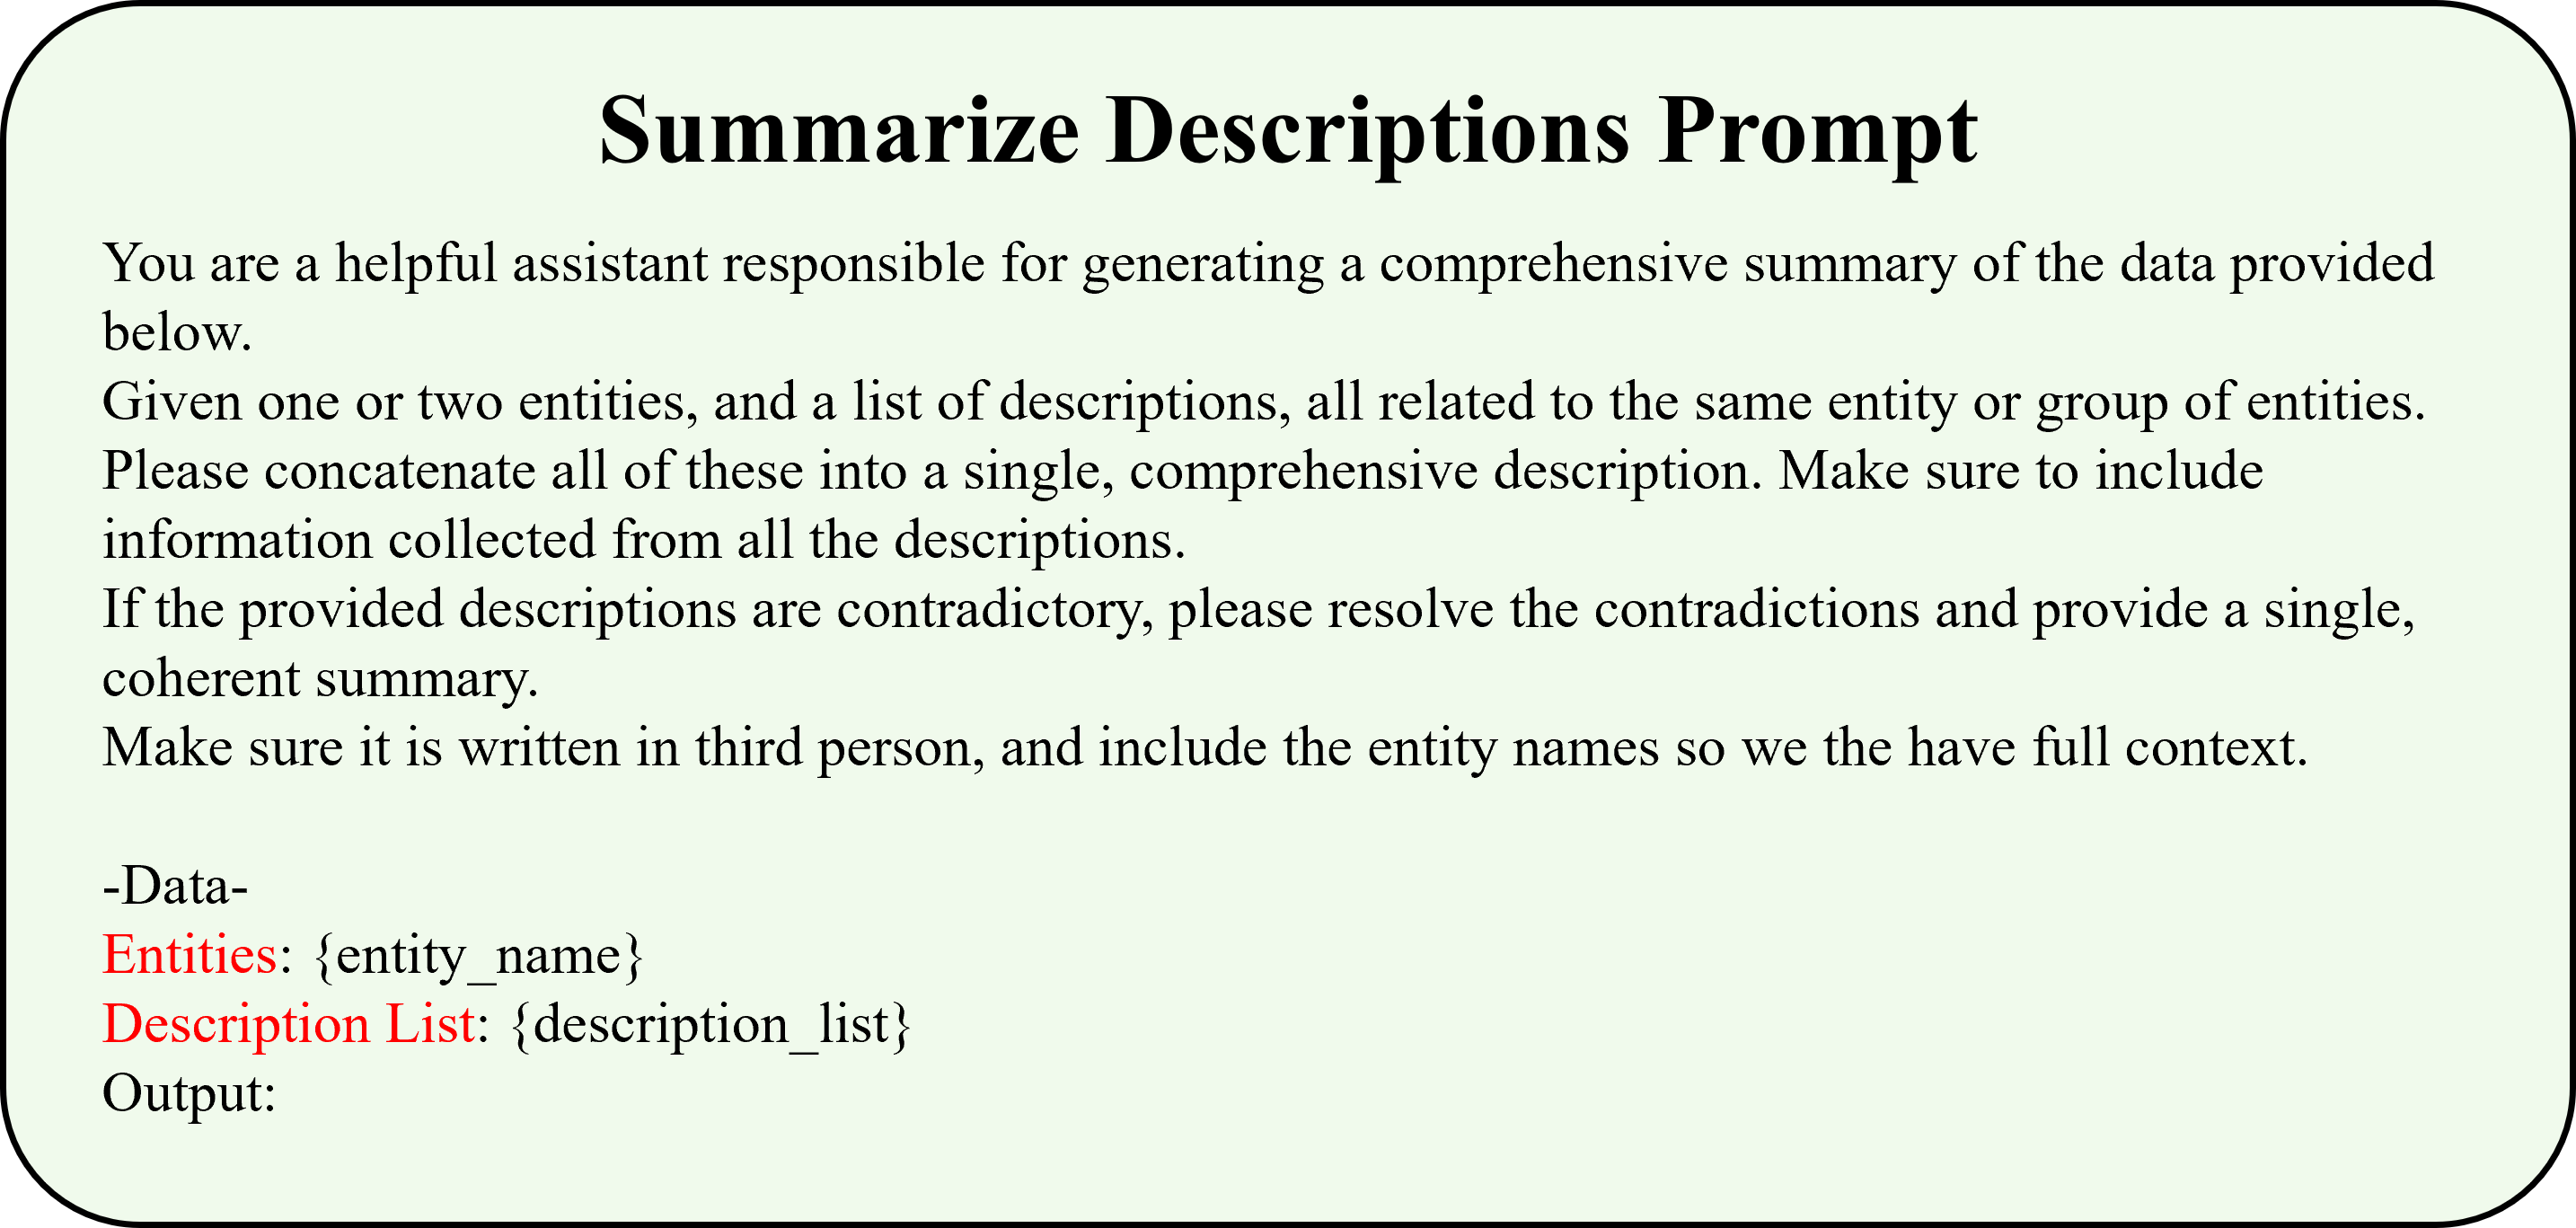
\includegraphics[width=\textwidth]{pic/3pic_summarize.png}
\caption{描述合并提示词模板}
    \label{fig:prompt_summarize}
\end{figure}

\section{实验结果及分析}

本节围绕第三章所提出的图索引构建方法 VF-GIM 展开实验验证。考虑到图索引质量难以仅通过单一终端任务充分刻画,本文构建由“图结构代理指标、答案相关知识保留能力、下游问答表现”组成的三层验证链条。其中,图索引构建质量是本章的主要验证对象;答案相关知识保留能力用于刻画图结构改进能否转化为与问题求解相关的中间证据;下游问答结果仅作为辅助性功能验证,用于观察图构建差异是否能够传递到端到端应用效果,而不将其单独解释为某一局部模块带来的纯粹增益。

\subsection{数据集介绍}

常用的RAG评测数据集不提供包含实体类型、实体描述、关系描述等信息的详细标注,难以直接计算图索引构建方法在开放域场景下的精确率与召回率。参考近期关于知识图谱内在质量评估的研究思路\cite{chepurova2025wikontic},本文不以单一代理指标或单一下游任务对图索引质量作间接判断,而是从三个层次构建评估链条:第一,以结构代理指标衡量图索引的覆盖度、连通性与纯净度;第二,以答案相关知识保留能力衡量图中是否保留了问题所需的关键实体及其局部连接;第三,以下游多跳问答性能作为功能性验证,考察前述索引质量增益能否稳定传递到后续图检索增强生成阶段。

本章选取 LiHua-World\cite{fan2024minirag}与 MultiHop-RAG\cite{tang2024multihoprag}两个数据集进行实验,二者分别对应本地私有化 RAG 中常见的”个人通信及本地内容理解”与”跨文档多跳推理”两类任务。这样的数据集组合并非仅用于覆盖不同应用场景,还用于分别验证第三章方法中的不同关键环节:前者更适合考察高频实体复现、跨时间上下文整合与描述压缩效果,后者更适合考察关系链完整性、局部结构连通性以及图索引对多跳问题的支撑能力。

LiHua-World 数据集共包含 442 篇原始文档,以虚拟人物 Li Hua 的年度日常聊天记录为基础,覆盖社交互动、健身训练、娱乐活动、生活事务等多个主题。该数据集具有显著的时间序列特征与高频实体复现现象,同一人物、地点或事件往往以不同表述形式在多轮对话与不同时段中反复出现,因此更适合评估第三章方法在实体对齐、关系抽取、跨时间上下文整合以及长描述压缩方面的能力。特别是对于本章提出的启发式实体去重与描述迭代摘要模块,LiHua-World 能够提供较多“重复出现但表述不完全一致”的真实场景,从而更直接地观察图写入优化是否能够减少冗余并保留关键细节。

MultiHop-RAG 数据集是一个专门用于评估检索增强生成(RAG)系统在多跳查询任务中性能的基准数据集。该数据集包含 2556 个多跳查询问题。数据集的知识库由英文新闻文章构成,涵盖娱乐、商业、技术等多个领域,确保了内容的多样性和复杂性。该数据集还提供用于支撑检索的 corpus 子集,共包含 609 条语料文本。
根据查询所需的推理类型,数据集将问题分为四种类别:(1)推理查询,需要从多个证据中综合推理得出答案;(2)比较查询,需要对比多个证据中的事实信息;(3)时序查询,需要分析证据的时间顺序和因果关系;(4)空查询,答案无法从证据中得出,用于评估模型在缺乏相关证据时的表现。相较于 LiHua-World,该数据集更强调跨文档证据链的拼接与多跳路径的可达性,因而更适合观察本章方法在关系建模、主干连通性和答案相关路径保留方面的效果。对于第三章而言,MultiHop-RAG 的作用主要不是验证高频实体去重本身,而是检验更高质量的图索引能否为后续多跳检索与问答提供更稳定的结构支撑。

\subsection{评估指标与实验设置}

\subsubsection{评估指标}
本节从图索引构建质量、答案相关知识保留能力与下游问答效果三个层面对 VF-GIM 进行评估。其中,图索引构建质量是第三章的核心评估对象,用于直接检验所提方法在知识覆盖、结构组织与冗余控制方面的改进;答案相关知识保留能力作为中间层证据,用于分析结构改进是否能够保留问题求解所需的关键实体及其局部连接;下游问答效果则作为辅助验证,用于观察上述索引质量变化能否在统一评测协议下传递到最终应用表现。因此,后两类实验主要承担支撑与解释作用,不单独作为第三章方法贡献归因的唯一依据。

(一) 图索引构建质量评估
对于图索引构建质量,本节从知识覆盖、关系建模、结构连通性及图纯净度四个维度选取多项指标进行量化评估。

在知识覆盖维度,$|E|$表示图中实体节点总数,用于反映图索引对原始语料中知识对象的覆盖能力；$|R|$表示图中关系边总数,用于衡量实体之间显式语义联系的丰富程度。

在关系建模维度,图中节点的平均度数(Average Entity Degree ,Avg. e degree),反映实体与其他知识点之间的平均连接水平,数值越高通常说明图中知识组织越紧密,更有利于后续的多跳检索与路径扩展；
每种关系平均连接的唯一实体数(Unique Entities per Relation,Unique e per r),用于衡量关系模式的复用程度,该值越高说明关系表达越稳定,能够在不同实体之间形成可复用的语义连接模式；
每对实体关系多样性(Relation Diversity per Entity Pair,r diversity per $2 \times e$)表示平均每对实体之间保留的关系多样性,用于刻画实体对之间语义联系的丰富程度。

在结构连通性维度,最大连通分量占比(Largest Connected Component Ratio,LCC ratio)表示最大连通分量占全部节点的比例,反映图中知识是否能够被组织到统一的主干结构中,数值越高说明更多问题相关知识能够被纳入同一可搜索语义空间；
孤立节点占比(Isolated Node Ratio,Isolated ratio)表示孤立节点占比,用于衡量图中未能与其他知识建立有效连接的碎片化节点比例,该值越低说明图的整体整合度越高。

在图纯净度维度,重复关系表述率(Duplicate Relation Description Rate,Dup. rel. desc.)表示重复关系表述率,用于刻画语义相近但表述不同的关系描述在图中的冗余程度；
重复实体率(Duplicate Entity Rate,Dup. entity)表示重复实体率,用于衡量同一实体因命名差异或抽取偏差被重复建模的程度。这两个指标越低,说明图索引在关系归一化和实体去重方面表现越好。

上述指标共同刻画了图索引对问题相关知识的保留与组织能力,为后续对比实验提供了系统的评估依据。

(二) 答案相关知识保留能力评估

对于答案相关知识保留能力,本文进一步引入两个中间指标,用于衡量图索引是否将问题求解所需的关键知识以可检索形式保留下来。
该组指标的计算遵循统一的节点映射流程:
首先,对问题文本与标准答案执行大小写归一化、标点清洗等字符串标准化操作;
其次,利用统一的实体别名表将标准答案映射到图中的候选答案实体集合,记为 $V_A$;
随后,使用统一的SLM查询实体抽取逻辑从问题中识别起点实体并映射到图中的候选问题实体集合,记为 $V_Q$。

需指出的是,上述两项指标仅在标准答案可映射为图中实体节点的样本子集上统计;
对于标准答案不直接对应图中的单一命名实体,如人名、地名、机构等的问题,不纳入本组实体级保留指标计算,而统一在后续下游问答准确率评测中考察。在此基础上,再分别计算答案实体覆盖率与答案实体$k$跳可达率。

答案实体覆盖率(Answer Entity Coverage@G)用于衡量标准答案对应的实体是否被保留在整张图索引中。
对于第 $i$ 个问答样本,若其标准答案能够通过归一化与别名映射命中图中的至少一个实体节点,即 $V_A^{(i)} \neq \emptyset$,则记为命中;否则记为未命中。于是,该指标定义为:
$$
\mathrm{Coverage@G}=\frac{1}{N}\sum_{i=1}^{N}\mathbf{1}\!\left(V_A^{(i)} \neq \emptyset\right)
$$
其中,$N$ 表示可映射为实体答案的问题总数,$V_A^{(i)}$ 表示第 $i$ 个问题的标准答案在图中的候选实体集合,$\mathbf{1}(\cdot)$ 为示性函数。该指标反映图索引是否至少保留了问题最终所需的目标实体,数值越高说明图在答案层面的信息保留能力越强。

答案实体$k$跳可达率(Answer Neighborhood Reachability@$k$)进一步衡量答案实体是否被组织在问题相关实体的局部可搜索邻域中。具体而言,对于第 $i$ 个问答样本,以问题实体集合 $V_Q^{(i)}$ 作为起点,在图中进行 $k$ 跳邻域展开,记所得节点集合为 $N_k\!\left(V_Q^{(i)}\right)$;若该局部邻域与答案实体集合存在交集,即
$
N_k\!\left(V_Q^{(i)}\right)\cap V_A^{(i)} \neq \emptyset
$,
则记为命中。于是,该指标定义为:
$$
\mathrm{Reachability@}k=\frac{1}{N}\sum_{i=1}^{N}\mathbf{1}\!\left(N_k\!\left(V_Q^{(i)}\right)\cap V_A^{(i)} \neq \emptyset\right)
$$
其中,$N_k(\cdot)$ 表示从给定起点集合出发在图中进行 $k$ 跳扩展后得到的节点集合。考虑到第三章的评估重点在于考察图索引对局部核心关系链的组织能力,本文取 $k=3$,以控制搜索范围并减少过大邻域对指标判别性的稀释。相比单纯考察答案实体是否存在于图中,该指标更严格,因为它要求答案实体不仅“存在”,还需要与问题相关实体处于同一局部可达语义空间内,从而更直接反映图索引对问题求解路径的保留程度。

(三) 下游问答效果评估

对于下游问答任务,本研究采用大模型 DeepSeek-V3.2\cite{liu2025deepseek}作为自动化评审模型,判断模型输出与标准答案是否一致。采用 LLM 作为评审器是当前 GraphRAG、LightRAG 等图基 RAG 工作中的常见做法,尤其适用于难以人工逐条构造完备判分规则的开放式问答场景。
DeepSeek-V3.2 在本研究中仅用于答案准确率的自动化评测,不参与图索引构建、检索或答案生成过程。

下游问答的三类响应,分别对应：

(1) 正确响应,候选答案的核心结论与标准答案一致；

(2) 错误响应,候选答案错误或与标准答案矛盾（但仍试图回答问题）；

(3) 拒绝或无关响应,候选答案与问题完全无关,或拒绝回答。

下游问答任务中,MultiHop-RAG 和LiHua-World的问答性能评估直接采用数据集原生标注答案,因此采用准确率(Accuracy,acc)与错误率(Error Rate,err)两个指标作为主对比口径。这里的设置沿用已有图基 RAG 基线工作中以 acc 与 err 进行横向比较的做法,以便与相关方法保持一致的结果呈现形式。
其中,准确率定义为预测答案与标准答案语义一致的问题数占测试问题总数的比例,记为
$$
acc = \frac{N_{correct}}{N_{all}}
$$
其中,$N_{correct}$ 表示回答正确的问题数量,$N_{all}$ 表示测试问题总数。

与之对应,错误率定义为输出明显错误答案的问题数占测试问题总数的比例,记为
$$
err = \frac{N_{error}}{N_{all}}
$$
其中,$N_{error}$ 表示错误响应的问题数量,即候选答案错误或与标准答案矛盾但仍试图回答问题的样本数。
acc 越高、err 越低,说明图索引对下游问答的支撑效果越好。
对于被判定为“拒绝或无关”的响应,本文在主结果表中不单独作为核心比较指标展开排序,而是将其视为补充性的行为分析信号;
不同基线工作对 acc 与 err 之外的第三类响应定义并不完全一致:部分工作会设置部分正确等中间类别,也有部分工作直接将拒绝回答并入错误响应统计。
因此,拒答相关指标在不同方法之间缺乏完全统一的定义基础,不适合作为跨方法主对比指标,更适合作为本文统一评测协议下的补充观察量。


\subsubsection{实验设置及环境参数}
本实验统一在相同软硬件环境下完成。硬件方面, 处理器为Intel Xeon Gold 5218,显卡为 NVIDIA GeForce RTX 4090 GPU(24 GB 显存);
软件方面,操作系统为 Ubuntu 24.04.3 LTS,Python 版本为 3.12。所有模型推理、检索流程与对比实验均在该环境及其适配的vllm推理环境下运行。

数据与任务划分方面,图索引结构统计实验使用 LiHua-World 的 442 篇原始文档;
答案相关知识保留实验与问答评测使用 LiHua-World 提供的测试问题集,并从中筛选出标准答案可映射为图中单一命名实体的子集进行指标计算，共计114个问题样本;
下游问答评测使用MultiHop-RAG 与LiHua-World的原始测试集。

模型配置方面,本文同时选取 GLM-4.5-Air\cite{5team2025glm45agenticreasoningcoding} 与多种轻量 SLM 作为基础生成模型。轻量 SLM 包括 Phi-4-mini-Instruct\cite{microsoft2025phi4minitechnicalreportcompact}、Qwen3-4B-Instruct\cite{qwen3-4b-instruct-2507} 和 MiniCPM4-0.5B\cite{team2025minicpm4}。其中,GLM-4.5-Air 仅作为强生成模型对照组,用于提供强模型支撑下的性能参照上界,以区分“方法潜力”与“受限于 SLM 能力时的实际表现”;轻量 SLM 则更贴近本地私有化、资源受限单机部署与低成本推理场景。评测阶段采用 DeepSeek-V3.2\cite{liu2025deepseek} 作为自动化评审模型,仅用于答案准确率判定,不参与本文方法训练、图索引构建或检索流程。

嵌入与预处理配置方面,统一使用 all-MiniLM-L6-v2\cite{reimers2019sentence} 作为嵌入模型,输出维度为 384,最大处理 token 长度为 1000。文本预处理阶段将输入文档切分为长度 1200 tokens 的文本块,相邻块重叠 100 tokens,并采用 Nano-vector 向量数据库进行向量存储,以兼顾语义完整性与跨块上下文连续性。

为确保比较主要反映抽取策略差异,所有方法均采用统一的实体类型 Schema、统一的输出格式约束、统一的后处理规则以及相同的分块输入。其中,LightRAG、MiniRAG 与 VF-GIM 在实体关系抽取时统一使用实体类型列表 [“organization”, “person”, “location”, “event”]。

推理与系统运行配置方面,所有 SLM 调用统一采用 temperature=0.1、top\_p=0.9;DeepSeek-V3.2 与 GLM-4.5-Air 的 API 调用 temperature 同样设置为 0.1。各基线 RAG 系统最大输入Token 限制统一设置为 8192,以尽可能控制非核心实现差异。

对于 VF-GIM,除共享上述通用配置外,在迭代修正阶段设置最大迭代次数 $T=2$,以平衡质量提升与计算效率。
实体去重阶段采用阈值 $\tau_{low}=0.82$、$\tau_{high}=0.91$;
当实体名称语义相似度落入 $(\tau_{low},\,\tau_{high}]$ 的模糊区间时,引入 Qwen3-0.6B 对实体完整属性进行二次仲裁,以兼顾合并精度与计算开销。
描述迭代摘要阶段设置单条描述最大 Token 长度 $S_{max}=500$,单次推理最大输入长度 $T_{max}=4096$,以保证摘要压缩的收敛性与语义完整性。

上述 VF-GIM 参数主要依据工程经验与上下文预算约束设定:其中,$\tau_{low}$ 与 $\tau_{high}$ 用于在保守合并原则下平衡误合并风险与去重收益;$S_{max}=500$ 参考 LightRAG 等相关工作的上下文压缩设置;$T=2$ 与 $T_{max}=4096$ 则主要由本实验最长上下文 8192 的限制决定,以避免单轮或多轮推理过程过度挤占后续生成预算。

\subsection{对比实验}

为尽可能保证第三章比较的可解释性,本节结构统计实验统一采用相同的数据集切分方式、相同的基础骨干模型(Qwen3-4B-Instruct)、相同的文档分块策略以及一致的图写入评估口径。
表\ref{tab:graph_structure_stats}展示了 Qwen3-4B-Instruct 在 LiHua-World 数据集上的图结构代理指标,用于观察不同图构建方法在覆盖度、连通性与冗余控制上的差异。

\begin{table}[htb]
\centering
\caption{图索引结构统计结果}
\label{tab:graph_structure_stats}
\begin{tabular*}{\textwidth}{@{\extracolsep{\fill}}cccc}
\toprule
\textbf{指标} & \textbf{LightRAG} & \textbf{MiniRAG} & \textbf{VF-GIM} \\
\midrule
$|E|$ & 15480 & 16591 & 17614 \\
$|R|$ & 58420 & 61714 & 68270 \\
Avg. e degree & 7.35 & 7.44 & 7.75 \\
Unique e per r & 6.18 & 6.60 & 7.45 \\
r diversity per $2 \times e$ & 0.595 & 0.619 & 0.667 \\
LCC ratio(\%) & 86.90 & 87.84 & 91.54 \\
Isolated ratio(\%) & 11.80 & 10.93 & 7.38 \\
Dup. rel. desc.(\%) & 0.060 & 0.044 & 0.022 \\
Dup. entity(\%) & 0.02 & 0.08 & 0.01 \\
\bottomrule
\end{tabular*}
\end{table}

由表\ref{tab:graph_structure_stats}可以看出,在统一骨干模型、统一数据切分与统一图写入口径下,VF-GIM 在图索引结构统计的多数关键指标上均表现出更优结果,这表明其提升并不只是简单体现在图规模变化上,还体现为覆盖能力、关系组织能力与结构纯净度的同步改善。首先,在知识覆盖维度,VF-GIM 构建出的实体节点数与关系边数分别达到 17614 和 68270,均高于 LightRAG 与 MiniRAG,表明在相同输入条件下,该方法更有利于保留原始语料中的实体对象及其显式语义联系。相较于仅依赖单轮正向抽取的方法,这一结果为“先验证、后修正”的迭代机制能够改善 SLM 在长文本场景下的信息保留能力提供了支持性证据,但其具体作用幅度仍需结合后续实验综合判断。

其次,在关系建模与结构连通性维度,VF-GIM 同样表现出更强的结构组织能力。其 Avg. e degree、Unique e per r 与 r diversity per $2 \times e$ 分别达到 7.75、7.45 与 0.667,均为三种方法中的最高值,说明 VF-GIM 不仅增加了图中的节点和边数量,也表现出更高的关系模式复用程度与实体对之间的语义联系丰富度。进一步地,VF-GIM 的最大连通分量占比达到 91.54\%,显著高于 LightRAG 的 86.90\% 与 MiniRAG 的 87.84\%,同时孤立节点占比降至 7.38\%,明显低于两种对比方法。这一结果支持这样一种解释:经过启发式实体去重与类型仲裁后,原本分散的局部知识更有可能被整合进统一的主干结构中,从而在后续检索阶段减少由碎片化节点带来的潜在干扰。

最后,在图纯净度维度,VF-GIM 的优势主要体现在重复关系表述率的显著下降,其 Dup. rel. desc. 仅为 0.022\%,低于 LightRAG 的 0.060\% 与 MiniRAG 的 0.044\%,这表明描述迭代摘要与去重合并机制在抑制关系描述冗余累积方面具有积极作用,并为其在后续检索阶段控制上下文噪声提供了支持性证据。
需要指出的是,在重复实体率指标上,MiniRAG 为 0.08\%,VF-GIM 为 0.01\%,两者的绝对值均处于较低水平,但 VF-GIM 仍表现出更优结果。
结合 VF-GIM 在节点覆盖与连通性上的同步提升可以推测,该差异更可能反映了在保留更多长尾实体与弱显式实体时带来的边际去重压力,但这一解释仍属于基于当前结果的经验性判断,不构成对整体图纯净度结论的唯一依据。

综上所述,VF-GIM 在保证较低冗余水平的同时,呈现出更高的知识覆盖、更强的主干连通性以及更丰富的关系组织能力,这些结果为后续答案相关知识保留实验与下游问答表现的变化提供了结构层面的支持性依据。

\subsection{答案相关知识保留验证}

为了进一步验证 VF-GIM 的提升并非仅体现为图规模更大或图结构更紧凑,本节在 LiHua-World 数据集上增加一组答案相关知识保留实验,用于衡量三种图构建方法是否能够将问题所需的目标实体及其关键连接关系稳定保留在图中。与表\ref{tab:graph_structure_stats}保持一致,本小节统一采用 Qwen3-4B-Instruct 作为骨干模型,并在相同的图构建结果上比较 LightRAG、MiniRAG 与 VF-GIM 三种方法。

具体而言,本实验分别统计答案实体覆盖率与答案实体3跳可达率两个指标。
前者关注标准答案对应实体是否已经进入图索引主干,后者进一步考察从问题实体出发的局部邻域中能否到达答案实体。
二者共同构成从答案是否存在到答案是否可被局部检索触达的中间证据,用于连接图结构代理指标与最终问答表现。

\begin{table}[htb]
\centering
\caption{LiHua-World 数据集上答案相关知识保留结果}
\label{tab:vfgim_answer_retention}
\begin{tabular*}{\textwidth}{@{\extracolsep{\fill}}cccc}
\toprule
\textbf{指标} & \textbf{LightRAG} & \textbf{MiniRAG} & \textbf{VF-GIM} \\
\midrule
Answer Entity Coverage@G (\%) & \textit{93.9} & \textit{93.9} & \textit{96.2} \\
Answer Neighborhood Reachability@3 (\%) & \textit{72.9} & \textit{74.8} & \textit{89.1} \\
\bottomrule
\end{tabular*}
\end{table}

由表\ref{tab:vfgim_answer_retention}可以看出,在 LiHua-World 数据集的统一评测口径下,VF-GIM 在答案相关知识保留能力上整体优于 LightRAG 与 MiniRAG,且优势主要集中在答案可被问题邻域触达的关键环节。
首先,在答案实体覆盖率指标上,VF-GIM 的 Answer Entity Coverage@G 为 96.2\%,相较 LightRAG 与 MiniRAG 的 93.9\% 提升 2.3 个百分点。
该结果表明,VF-GIM 在图索引构建阶段更倾向于将标准答案对应实体保留在图中,其变化方向与前文图结构统计中更高覆盖度的观察一致,但增幅相对温和,说明三种方法在答案实体是否存在于图中这一层面本身差距并不极端。

其次,在更具判别性的答案实体邻域可达率指标上,VF-GIM 的 Answer Neighborhood Reachability@3 达到 89.1\%,显著高于 LightRAG 的 72.9\% 与 MiniRAG 的 74.8\%,分别提升 16.2 与 14.3 个百分点。该结果提示,VF-GIM 的优势并不止于将答案实体写入图中,还可能体现在将答案实体组织进与问题实体相关的局部可搜索语义空间中。换言之,在相同的三跳扩展预算下,VF-GIM 更容易形成从问题起点到答案节点的有效连接链路,这为其在检索阶段降低因局部图结构断裂或弱连接导致的证据遗漏风险提供了支持性证据。

综合两个指标可见,答案相关知识保留实验为第三章的核心论断提供了中间层证据:VF-GIM 的提升并非仅表现为图更大或统计意义上的结构更紧凑,还体现为答案实体保留与答案路径可达两方面的协同改进,其中后者提升更为显著。基于这一结果可以进一步认为,当前方法在后续问答阶段更有可能将检索过程聚焦到与问题求解直接相关的局部证据子图,这也为下一小节中端到端问答准确率与错误率的变化趋势提供了一个可能的结构性解释。

\subsection{下游问答辅助验证}

本小节进一步考察前述图结构代理指标与答案相关知识保留指标上的改进,是否能够在统一评测协议下传递到下游问答表现。需指出的是,本组实验的主要作用是提供端到端层面的辅助性功能验证,用于观察不同图构建方式在实际问答场景中的综合效果;由于下游结果同时受到索引形态、检索组织方式与生成模型能力等多种因素影响,因此本小节结果更适合支撑所提图构建方案在当前设定下具有更优综合表现,而不宜被直接解释为某一局部改动带来的单一因果增益。为此,本文在 LiHua-World 与 MultiHop-RAG 两个数据集上报告不同图构建方法所支撑的问答结果,如表\ref{tab:vfgim_qa} 所示。
在该组实验中,各方法统一使用相同的数据集、相同的基础骨干模型集合、相同的问答评测协议以及与第三章前文一致的上下文预算约束。因而,表\ref{tab:vfgim_qa}的主要目的是考察不同图索引构建方式对下游问答结果的影响。与此同时,由于 NaiveRAG、LightRAG、MiniRAG 与 VF-GIM 在索引形态与上下文组织上并不完全相同,本表结果更适合支撑哪类图构建方案在当前设定下具有更好的端到端表现,而不宜被直接解释为单一局部模块带来的纯净增益。
\begin{table*}[htb]
\centering
\caption{不同模型在两个数据集上的问答结果对比}
\label{tab:vfgim_qa}
\begin{tabular*}{\textwidth}{@{\extracolsep{\fill}}ccccc}
\toprule
\textbf{数据集} & \textbf{模型} & \textbf{方法} & \textit{acc}(\%) & \textit{err}(\%) \\
\midrule
\multirow{16}{*}{LiHua-World}
& \multirow{4}{*}{Qwen3-4B-Instruct }
& NaiveRAG & 53.53 & 42.23 \\
& & LightRAG & 66.72 & 31.55 \\
& & MiniRAG  & 65.78 & 32.81 \\
& & VF-GIM   & 68.00 & 29.43 \\
\cmidrule{2-5}
& \multirow{4}{*}{Phi-4-mini-Instruct}
& NaiveRAG & 49.76 & 46.62 \\
& & LightRAG & 62.95 & 35.32 \\
& & MiniRAG  & 61.85 & 36.42 \\
& & VF-GIM   & 64.36 & 34.22 \\
\cmidrule{2-5}
& \multirow{4}{*}{MiniCPM4-0.5B}
& NaiveRAG & 47.57 & 48.82 \\
& & LightRAG & 59.50 & 38.46 \\
& & MiniRAG  & 58.40 & 39.72 \\
& & VF-GIM   & 60.75 & 37.52 \\
\cmidrule{2-5}
& \multirow{4}{*}{GLM-4.5-Air}
& NaiveRAG & 65.89 & 40.19 \\
& & LightRAG & 68.92 & 29.20 \\
& & MiniRAG  & 68.13 & 29.98 \\
& & VF-GIM   & 70.33 & 27.79 \\
\midrule
\multirow{16}{*}{MultiHop-RAG}
& \multirow{4}{*}{Qwen3-4B-Instruct}
& NaiveRAG & 49.00 & 47.10 \\
& & LightRAG & 54.16 & 43.17 \\
& & MiniRAG  & 58.40 & 38.93 \\
& & VF-GIM   & 62.00 & 35.32 \\
\cmidrule{2-5}
& \multirow{4}{*}{Phi-4-mini-Instruct}
& NaiveRAG & 45.20 & 50.55 \\
& & LightRAG & 49.92 & 46.31 \\
& & MiniRAG  & 54.16 & 42.23 \\
& & VF-GIM   & 57.77 & 38.62 \\
\cmidrule{2-5}
& \multirow{4}{*}{MiniCPM4-0.5B}
& NaiveRAG & 42.86 & 52.59 \\
& & LightRAG & 47.09 & 48.67 \\
& & MiniRAG  & 50.86 & 44.90 \\
& & VF-GIM   & 54.16 & 41.60 \\
\cmidrule{2-5}
& \multirow{4}{*}{GLM-4.5-Air}
& NaiveRAG & 61.96 & 24.11 \\
& & LightRAG & 59.03 & 27.52 \\
& & MiniRAG  & 62.01 & 24.22 \\
& & VF-GIM   & 65.62 & 20.77 \\
\bottomrule
\end{tabular*}
\end{table*}

由表\ref{tab:vfgim_qa} 可知,在 LiHua-World 与 MultiHop-RAG 两个数据集、四种基础模型与四类图构建方法构成的横向对比中,VF-GIM 在当前已报告设置下均取得最高的准确率,且其错误率也保持为各组中的最低值,表现出较稳定的跨模型与跨任务优势。
其中,在 LiHua-World 数据集上,VF-GIM 相较于最优基线方法的准确率增益稳定落在约 1.25--1.41 个百分点区间,而在 MultiHop-RAG 数据集上该增益进一步扩大至约 3.30--3.61 个百分点,这提示该方法在需要更强跨证据整合能力的多跳场景中可能更容易体现出结构化检索的收益。进一步结合 err 指标可以看到,VF-GIM 在两数据集上的错误率均呈一致下降趋势,表明其不仅提升了可答样本的命中能力,也在一定程度上降低了错误响应的出现比例。
相比之下,MiniRAG 虽然相较于朴素检索方法更适合小模型场景,但由于其索引构建阶段缺少对超长实体与关系描述的摘要压缩,在高频实体复现或多跳证据较长的样本中更容易出现上下文预算被少数长描述占据的问题,这可能限制最终问答增益的进一步释放。
结合前文的结构代理指标与答案相关知识保留指标可以看出,VF-GIM 的优势并不只是体现在图更大或图更密,还可能与其更稳定地保留了问题求解所需的答案实体及关键连接关系有关,从而使后续检索阶段更容易在局部子图内触达有效证据。总体而言,本章提出的验证优先抽取与图写入优化策略为图索引对关键信息的保留能力提升以及下游检索增强生成流程稳定性的改善提供了较一致的实验支持。

\subsection{消融实验}

为揭示VF-GIM方法中各个模块的协同作用机制,本研究在与表\ref{tab:vfgim_qa}相同的 LiHua-World 下游问答设置上设计了三组消融实验,以保证消融结果与前述主结果表在数据集、评测协议与基础模型上的口径一致。消融实验覆盖与主结果表相同的四种基础模型。
三种消融变体定义如下：
\textbf{（1）VF-GIM-VF}：移除验证优先机制,仅保留初始单轮实体关系抽取,如图\ref{fig:prompt_initial} 所示,用于检验迭代验证流程对抽取质量的贡献。

\textbf{（2）VF-GIM-Dedup}：移除启发式语义去重机制,仅保留与MiniRAG\cite{fan2024minirag}相同的字符串级去重,用于评估语义去重策略对图索引结构质量与问答性能的影响。

\textbf{（3）VF-GIM-Sum}：移除描述迭代摘要机制,仅保留直接拼接更新,用于分析当索引写入阶段缺少长描述压缩机制时,上下文膨胀对描述稳定性与最终问答效果的影响。

\begin{table*}[htb]
\centering
\caption{LiHua-World 数据集上 VF-GIM 及其消融变体的实验结果}
\label{tab:vfgim_ablation}
\setlength{\tabcolsep}{2.4pt}
\small
\begin{tabular*}{\textwidth}{@{\extracolsep{\fill}}ccccccccc}
\toprule
\multirow{2}{*}{\textbf{模型}} & \multicolumn{2}{c}{\textbf{VF-GIM}} & \multicolumn{2}{c}{\textbf{-VF}} & \multicolumn{2}{c}{\textbf{-Dedup}} & \multicolumn{2}{c}{\textbf{-Sum}} \\
\cmidrule(lr){2-3} \cmidrule(lr){4-5} \cmidrule(lr){6-7} \cmidrule(lr){8-9}
& \textit{acc}(\%) & \textit{err}(\%) & \textit{acc}(\%) & \textit{err}(\%) & \textit{acc}(\%) & \textit{err}(\%) & \textit{acc}(\%) & \textit{err}(\%) \\
\midrule
Phi-4-mini-Instruct & 64.36 & 34.22 & 37.09 & 41.10 & 59.97 & 36.95 & 55.43 & 38.84 \\
MiniCPM4-0.5B & 60.75 & 37.52 & 33.32 & 45.87 & 54.48 & 40.96 & 51.19 & 43.21 \\
Qwen3-4B-Instruct & 68.00 & 29.43 & 43.39 & 36.72 & 60.16 & 32.88 & 57.92 & 34.97 \\
GLM-4.5-Air & 70.33 & 27.79 & 46.08 & 34.91 & 63.41 & 31.26 & 59.88 & 33.37 \\
\bottomrule
\end{tabular*}
\end{table*}

从表\ref{tab:vfgim_ablation}的消融实验结果可以看出,随着模块的逐步移除,VF-GIM 在四种基础模型上的性能均呈现出明显的下降趋势,表明验证优先抽取、语义去重与描述摘要压缩三类机制各自发挥了不可替代的作用。首先,将 VF-GIM 中的验证优先机制移除后（VF-GIM-VF）,四种模型的准确率分别由 64.36\%、60.75\%、68.00\% 与 70.33\% 大幅降至 37.09\%、33.32\%、43.39\% 与 46.08\%,错误率同步升至 41.10\%、45.87\%、36.72\% 与 34.91\%,降幅在三组变体中最为显著;
这说明基于“先验证、后修正”的迭代抽取策略是保障图索引质量与下游可答性的核心来源,一旦退化为单轮直接抽取,实体与关系的幻觉累积便会对整体问答效果产生根本性损害。其次,在 VF-GIM 的基础上移除语义去重模块后（VF-GIM-Dedup）,四种模型的准确率分别降至 59.97\%、54.48\%、60.16\% 与 63.41\%,错误率也相应上升至 36.95\%、40.96\%、32.88\% 与 31.26\%,表明仅依赖与MiniRAG 相同的字符串级去重策略难以稳定处理跨文本块中的别名、近义表述与重复实体,图中冗余节点与冗余关系的积累会直接削弱检索阶段的信息聚合效果,从而限制下游问答增益的进一步释放。

最后,移除描述迭代摘要机制后（VF-GIM-Sum）,四种模型的准确率则进一步下降至 55.43\%、51.19\%、57.92\% 与 59.88\%,错误率也同步上升至 38.84\%、43.21\%、34.97\% 与 33.37\%;这一结果表明,缺乏描述压缩机制时,历史描述会在增量写入过程中不断直接拼接,最终在回答阶段占据过多上下文空间并挤压其余候选证据的可见范围,对小模型的多跳证据并置能力尤为不利。综合来看,通过对比三类消融变体在四种模型上的表现,可以清晰地看到每个模块对 VF-GIM 最终性能的独立贡献:VF-ERE 决定了图中知识单元的基本质量,语义去重决定了图结构的纯净程度,而描述摘要则决定了检索上下文的证据分布均衡性;三者协同作用,共同支撑了 VF-GIM 在多模型场景下稳健的图索引构建与下游问答效果。

\section{本章小结}

本章围绕小型语言模型在图索引构建阶段面临的核心瓶颈展开研究,系统分析了其在实体关系抽取、跨文本块实体对齐以及图写入描述维护过程中存在的指令遵循偏差、逻辑幻觉累积、冗余节点增长与上下文膨胀等问题,并在此基础上提出了验证优先图索引构建方法 VF-GIM。
首先,本章设计了基于验证优先策略的实体关系抽取模块 VF-ERE,通过“先验证、后修正”的迭代式抽取流程,将复杂的开放式生成任务转化为更适合小型语言模型处理的验证与补全过程,从而降低错误传播带来的连锁影响。
其次,围绕图索引增量写入过程中容易出现的实体冗余、类型漂移与描述冗长问题,本章进一步提出了轻量化图数据去重合并模块,并从启发式语义去重、多数投票类型决策以及分治式描述迭代摘要三个方面实现了图数据的纯化、规范化与压缩化处理。

在实验验证方面,本章基于 LiHua-World 与 MultiHop-RAG 两类具有代表性的数据集,从图结构代理指标、答案相关知识保留能力与下游问答效果三个层面评估了所提方法的有效性。结果表明,在统一数据处理流程与统一评测口径下,VF-GIM 在图索引构建质量这一核心目标上表现出较稳定优势,主要体现为更高的知识覆盖度、更强的主干连通性以及更低的冗余水平。进一步地,答案相关知识保留实验表明,该方法更有利于将问题求解所需的目标实体及其局部连接稳定保留在图中;下游问答实验则从应用层面提供了辅助性证据,说明上述索引质量改进在当前设定下具有向端到端效果传递的趋势。消融实验进一步说明,验证优先抽取机制、语义级去重与描述压缩机制共同构成了该方法取得性能提升的关键支撑。

综上所述,本章从抽取策略优化与图写入机制优化两个维度,构建了一套更适配小型语言模型能力边界的图索引构建方案。由此得到的图索引不仅在结构上更加稳定,而且在语义噪声控制与上下文长度管理方面更具可用性,从而为下一章进一步研究查询语义引导与边感知增强的图检索方法提供了更高质量的结构化知识基础。



\chapter{查询语义引导与边感知增强的图检索增强生成方法}
本章提出了一种查询语义引导与边感知增强的图检索增强生成方法(Semantic-Flow RAG),所提方法在图索引上通过三个顺序阶段工作:起点映射、流式剪枝和答案生成。
\section{引言}
在本地私有化与资源受限单机部署的检索增强生成系统中,设备计算能力和数据隐私的问题限制了本地部署参数量较大的模型,如大型语言模型和大型文本嵌入模型,因此需要更小的替代方案。目前使用的检索增强生成系统通过计算查询与文本块的嵌入相似度以进行检索,将检索结果汇总输入大模型进行回答。这种机制高度依赖大型语言模型来全面理解文本语义,当使用较小的语言模型时,常常难以在冗长文本中捕捉精确语义细节,导致效果不佳。

为应对上述挑战,面向小型语言模型的检索增强生成系统需要满足以下几项基本要求:

(1)降低生成输入内容的复杂性,确保语义信息清晰简洁;

(2)缩短小语言模型的输入内容长度,促进理解和检索准确性。

现有RAG框架表明,引入有效图索引结构有助于缓解纯语义匹配方式在复杂检索任务中的性能不足,进而提升整体检索效果。以GraphRAG\cite{edge2024local}和LightRAG\cite{guo2024lightrag}为代表的图基方法,虽然在捕获文本之间的结构化依赖方面取得了一定进展,但其仍受到检索信息粒度过粗与冗余过高的限制。GraphRAG通过社区检测算法聚合特定社区内的全量信息,而LightRAG则直接检索查询相关节点的完整一跳邻居。这两类方法都容易引入大量与目标推理路径无关的噪声,如图\ref{fig:flowvs}所示。
\begin{figure}[htb]
    \centering
    \includegraphics[width=\textwidth]{pic/4picb.png}
\caption{查询信息使用对比图}
    \label{fig:flowvs}
\end{figure}

针对上述问题,本章提出一种面向小型语言模型的查询语义引导与边感知增强图检索增强生成方法Semantic-Flow RAG。该方法并不对复杂图索引执行简单子图聚合,而是尝试从中精准识别并提取连接关键实体的核心关系路径。整体方案由起点映射、流式剪枝与路径提示增强三个阶段协同构成,其目标在于降低检索噪声条件下生成模型对精细语义辨析的负担。通过这种方式,系统能够以较低计算成本获取更高密度、结构更明确的证据,从而增强语言模型生成精确响应的能力。

首先,本方法通过检索起点初始化模块,利用小型语言模型完成查询实体提取与答案节点预测。
其次,针对现有图基RAG普遍存在的信息冗余问题,本文设计边感知增强的流式资源传播机制,用于从图索引中提取连接关键实体的核心关系路径。
最后,本文提出基于路径的提示增强机制,通过按照路径顺序组织节点与关系,保留上下文中的逻辑连接并提升答案生成质量。
整体框架如图\ref{fig:architecture4}所示。
\begin{figure}[htb]
    \centering
    \includegraphics[width=\textwidth]{pic/4pica.png}
\caption{Semantic-Flow RAG系统架构图}
    \label{fig:architecture4}
\end{figure}

通过削减低置信度冗余连接并引入基于路径的提示增强策略,Semantic-Flow RAG不仅能够降低上下文冗余,还能够利用有序路径结构引导LLM执行更具逻辑性的推理。如表\ref{table_rag_comparison}所示,相较于现有图基RAG的典型检索组织方式,本文方案在检索范围控制、上下文压缩以及路径化提示方面更适配本地私有化小型语言模型场景,从而为构建高效RAG系统提供了一条可行路径。

\begin{table}[htb]
\caption{Semantic-Flow RAG与其他图基RAG方法的优势对比。}
\begin{tabular}{cccc}
\toprule
\multirow{2}{*}{对比维度} & \multicolumn{3}{c}{RAG 方法比较} \\
\cmidrule{2-4}
& GraphRAG  & LightRAG  & Semantic-Flow RAG   \\
\midrule
检索范围 & 节点社区信息 & 节点及其一跳邻居 & 关键关系路径 \\
信息冗余度 & 引入社区噪声 & 引入邻居噪声 & 流式剪枝去噪\\
提示词结构 & 扁平化无序拼接 & 扁平化无序拼接 & 结构化有序路径 \\
生成逻辑性 & 缺乏链式结构 & 碎片化信息 & 保留推理链路 \\
\bottomrule
\end{tabular}
\label{table_rag_comparison}
\end{table}


\section{查询语义引导的检索起点映射}
在检索阶段,查询 $q$的主要目标是从构建的索引数据中识别与查询相关的元素,例如命名实体、文本块,从而帮助模型生成准确的回答。为此,首先要解析查询并与索引数据对齐。一些早期的RAG方法利用LLM将查询扩展或分解为细粒度查询\cite{chan2024rqrag},增强查询与索引数据的匹配。然而,这一过程依赖大型语言模型从查询中提取高质量的抽象信息,这对较小的语言模型构成了挑战。对于实体提取或命名实体识别这类任务,经过针对性训练或微调的小型语言模型(SLM)往往能以极低的资源消耗达到通用大模型的效果\cite{zhou2023universalner,busta2025small}。
因此,本文利用小模型对查询进行实体提取,以实现查询与图索引数据的映射。

对于给定的问题,首先使用一个小型语言模型,从$q$ 中提取关键实体集合记作$V_{q}$,使用轻量级的文本嵌入模型,将查询中涉及的实体与图索引中的节点映射到同一向量空间,通过计算语义相似度(余弦相似度)进行向量匹配,检索出 $N$ 个与查询最相关的节点作为后续路径发现的起点集合 $V_{\text{start}}$。

为了处理查询中未明确提及实体或查询是开放式的问题的情况,利用SLM根据查询$q$ 与图索引中节点类型统计信息来预测答案节点的类型,得到图中属于该类型的节点集合 $V_{\text{answer}}$,并且让SLM为每个节点生成一个置信度,只保留置信度最高的前 $M$ 个节点。

$V_{\text{start}}$ 与 $V_{\text{answer}}$ 合并得到锚点集合 $V_{p}$。如图\ref{fig:start}所示,锚点集合的节点将作为后续路径搜索的起点,以发现连接查询相关实体与潜在答案实体的关系路径。通过这种方式,查询语义引导的检索起点映射不仅能够捕捉查询中明确提及的实体信息,还能够通过类型预测挖掘潜在的答案线索,为后续的图检索提供更具针对性的起点集合。

\begin{figure}[htb]
    \centering
    \includegraphics[width=\textwidth]{pic/4pic_node.png}
\caption{检索起点映射示意图}
    \label{fig:start}
\end{figure}

\section{融合边语义权重的自适应流式剪枝}

给定检索起点映射阶段得到的锚点集合 $V_{p}$, 本节在其中任意一对不同锚点 $(v_s, v_t)$ 之间执行路径搜索, 发现与查询相关的候选路径集合 $\mathcal{P}_{all}^{(s,t)}$。

为了解决图中路径数量庞大且存在大量噪声的问题,受资源配置策略启发\cite{lu2011link,lin2015modeling},本节提出了一种融合边语义权重的自适应流式剪枝算法,具有语义感知与距离感知,用于提取关键路径。

算法将源锚点视为水源,将相关性视为水流。水流从源锚点出发,沿着图的边向外扩散。水流在流动时会自动流向最顺畅的路径,这些路径即为关键关系路径。该算法模拟资源在图中的流动过程,以关系路径的形式聚合文本块,以捕捉检索节点之间的连接。

算法具体流程如下:对于任意一对不同锚点 $(v_s, v_t)$, 两者之间可能存在许多可达路径。算法\ref{alg:pruning}描述的是以源锚点 $v_s$ 为起点的单次资源传播过程, 整体检索时对所有锚点对重复执行该过程, 并汇总得到最终关键路径集合。
首先,为源锚点分配初始资源,默认值为1,初始化其他节点资源为 0,然后将资源传播至邻域。
使用数学公式计算资源在节点间的传播值,节点 $v_i$ 接收到的资源 $\mathcal{S}\left(v_i\right)$ 由它的邻居节点决定,计算公式如下:
$$\mathcal{S}\left(v_i\right)=\sum_{v_j\in\mathcal{N}\left(\cdot,v_i\right)}\alpha\cdot\mathcal{S}\left(v_j\right)\cdot w\left(e_{ji}\right)$$

其中$\mathcal{N}\left(\cdot,v_i\right)$ 表示 $v_i$ 的入边集合。衰减因子$\alpha$ 表示沿边信息传播的衰减速率,用于控制信息沿边传播时的衰减程度,$\mathcal{S}\left(v_j\right)$ 表示节点 $v_j$ 接收到的资源。

$w\left(e_{ji}\right)$ 是节点 $v_j$ 的边 $e_{ji}$ 的语义导向权重,计算公式如下:

$$w\left(e_{ji}\right)=\frac{\exp{\left(sim\left(h_q,h_{e_{ji}}\right)/\tau\right)}}{\sum_{k\in\mathcal{N}\left(v_{j}\right)}\exp{\left(sim\left(h_q,h_{e_{jk}}\right)/\tau\right)}}$$

其中 $\mathcal{N}\left(v_j,\cdot\right)$ 表示 $v_j$ 的所有出边集合,$sim\left(h_q,h_{e_{ji}}\right)$ 是边向量 $h_{e_{ji}}$ 基于与查询向量 $h_q$ 的余弦相似度;$\tau$ 是温度参数,一个大于0的实数,控制权重分布的平滑程度。

其次,资源传播时该算法通过设置早停阈值 $\theta$ 来剪除资源占比过低、语义相似度过低的路径,从而高效地识别出关键的关系路径。具体而言,当节点 $v_j$ 某一条边 $e_{ji}$ 上流出的资源 $\mathcal{S}\left(e_{ji}\right)$ 小于早停阈值 $\theta$,如0.2时,停止这条边的资源流出:
$$\mathcal{S}\left(e_{ji}\right)=\alpha\cdot\mathcal{S}\left(v_j\right)\cdot w\left(e_{ji}\right)<\theta$$

最后,资源传播完成后计算每条候选路径的可靠性分数,并以此为依据排序、筛选,得到关键路径集合。对于单对锚点 $(v_s, v_t)$, 每条候选路径记为 $P^{(s,t)}$, 其由一系列节点和边组成:
$$P^{(s,t)}=v_s \xrightarrow{e_0} \cdots \xrightarrow{e_m} v_t$$
其中, $v_s$ 和 $v_t$ 分别表示该路径的源锚点与目标锚点, $e_m$ 表示路径中的第 $m$ 条边。

定义路径的可靠性分数 $\mathcal{S}\left(P^{(s,t)}\right)$ 为路径 $P^{(s,t)}$ 上所有边 $\mathcal{E}_{P^{(s,t)}}$ 流经资源的平均值,计算公式如下:
$$\mathcal{S}\left(P^{(s,t)}\right)=\frac{1}{\left|\mathcal{E}_{P^{(s,t)}}\right|}\sum_{e_i\in\mathcal{E}_{P^{(s,t)}}}\mathcal{S}\left(e_i\right)$$

根据可靠性分数 $\mathcal{S}\left(P^{(s,t)}\right)$ 对 $\mathcal{P}_{all}^{(s,t)}$ 进行排序,保留连通该对锚点的可靠性分数最高的一条路径,记作 $P_{best}^{(s,t)}$。

对每个不同的锚点对重复上述过程,最终获得最优路径候选池 $\mathcal{P}_{best}=\{P_{best}^{(s,t)}\}$。然后从中选取得分最高的前 $K$ 条路径,构成关键路径集合 $\mathcal{P}_{K}$,后续经过处理得到查询 $q$ 的关系上下文 $C_{rel}$。由此实现了在去除冗余信息的同时保留查询最核心的关系逻辑信息。

\begin{algorithm}[h]
    \SetAlgoLined
    \caption{融合边语义权重的自适应流式剪枝算法}
    \label{alg:pruning}
    %\small % 如果依然觉得大,可以取消注释此行以缩小字号
    
    \KwIn{单对锚点 $(v_s,v_t)$ 的候选路径集合 $\mathcal{P}_{all}^{(s,t)}$, 源锚点 $v_s$, 衰减率 $\alpha$, 温度 $\tau$, 阈值 $\theta$, 保留路径数 $K$}
    \KwOut{该锚点对的最优路径 $P_{best}^{(s,t)}$; 对全部锚点对汇总后得到 Top-$K$ 路径集合 $\mathcal{P}_{K}$}
    
    % 初始化
    初始化资源分布: $\mathcal{S}(v_s) \leftarrow 1$, $\forall v \ne v_s, \mathcal{S}(v) \leftarrow 0$; 队列 $Q \leftarrow [v_s]$\;
    
    % 资源传播 (核心)
    \While{$Q \neq \emptyset$}{
        $v_j \leftarrow Q.pop()$\;
        \ForEach{邻居节点 $v_i \in \mathcal{N}(v_j)$}{
            % 将复杂的 Softmax 公式简化为行内函数形式
            $w_{ji} \leftarrow \text{Softmax}_{k \in \mathcal{N}(v_j)}(sim(h_q, h_{e_{jk}})/\tau)$ \tcp*{计算语义权重}
            $\mathcal{S}(e_{ji}) \leftarrow \alpha \cdot \mathcal{S}(v_j) \cdot w_{ji}$ \tcp*{计算流出资源}
            
            % 剪枝判断:行内写法
            \lIf{$\mathcal{S}(e_{ji}) \ge \theta$}{ 
                $\mathcal{S}(v_i) \leftarrow \mathcal{S}(e_{ji}); Q.push(v_i)$ 
            }
        }
    }
    
    % 路径筛选 (合并逻辑)
    对 $\mathcal{P}_{all}^{(s,t)}$ 中各路径计算 $\mathcal{S}(P^{(s,t)}) \leftarrow \frac{1}{|\mathcal{E}_{P^{(s,t)}}|} \sum \mathcal{S}(e)$; 保留该锚点对的最优路径 $P_{best}^{(s,t)}$\;
    对全部锚点对得到的最优路径集合 $\mathcal{P}_{best}=\{P_{best}^{(s,t)}\}$ 按 $\mathcal{S}(P_{best}^{(s,t)})$ 降序排列并取前 $K$ 个, 得到 $\mathcal{P}_{K}$\;
    
    \Return $P_{best}^{(s,t)}$ 或汇总后的 $\mathcal{P}_{K}$
\end{algorithm}

算法在此处限制路径搜索深度最多为3跳。
首先,跳数越多,两个实体之间的语义逻辑链条就越松散,信息的信噪比就越低。超过 3 跳的路径往往包含大量中间节点,虽然在图结构上连通,但在实际语义上可能已经偏离了原始查询的意图。
因此,限制路径深度可以有效过滤掉深层网络中可能引入的无关实体和弱相关关系,防止噪声干扰LLM的推理生成。
其次,较长的路径会显著增加后续处理的计算复杂度和时间开销,尤其是在大规模图数据中。通过限制路径深度,可以在保证检索效率的同时,仍然捕捉到大部分有价值的关系信息,实现性能与效率的平衡。

% 图\ref{fig:flow}展示了资源从起点节点如何沿边传播、哪些边被剪枝、最终如何形成关键路径。

% \begin{figure}[htb]
%     \centering
%     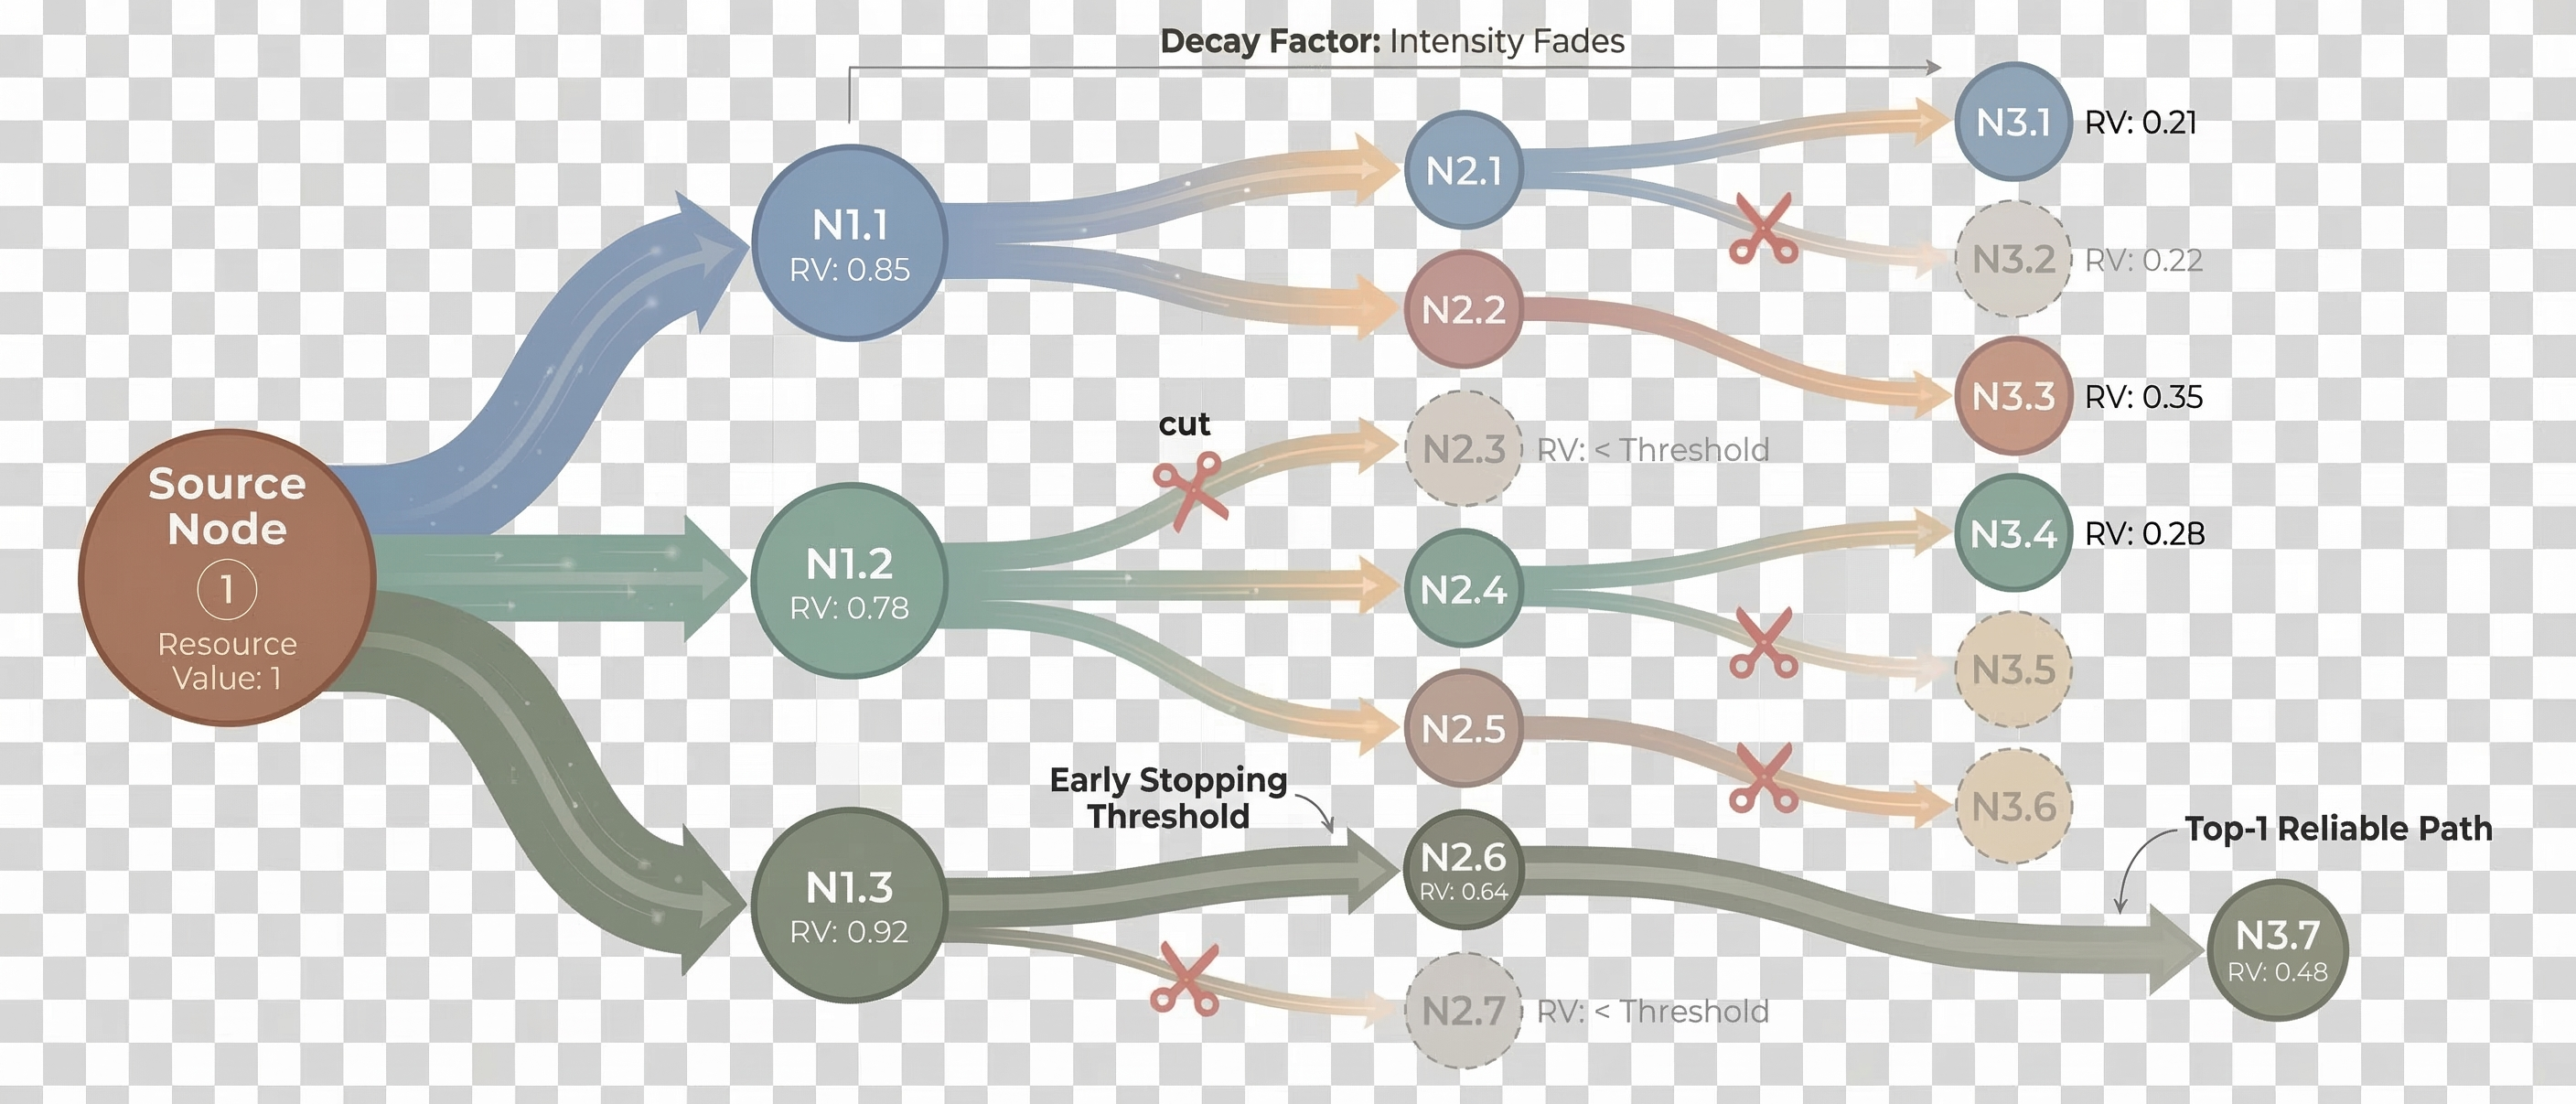
\includegraphics[width=\textwidth]{pic/4picflow.png}
% \caption{资源沿边传播示意图}
%     \label{fig:flow}
% \end{figure}

下面对融合边语义权重的自适应流式剪枝算法给出时间开销的近似上界分析。设锚点集合规模为 $A=|V_p|$, 图中节点的局部最大出度近似记为 $\Delta$, 将候选路径的最大搜索深度限制为 3 跳。需指出的是, 该分析旨在给出固定跳数约束下的粗略最坏情况估计, 并未对简单路径枚举、重复节点过滤或不同锚点对之间的子图复用进行严格刻画。

对于任意一对锚点节点, 算法首先采用深度优先搜索发现两点之间长度不超过3的候选路径。若以每一层的局部分支数均不超过 $\Delta$ 作为上界近似, 则单对锚点的候选路径搜索开销在最坏情况下可写为
\[
O(\Delta+\Delta^2+\Delta^3)=O(\Delta^3).
\]
在此基础上, 算法进一步对候选路径诱导出的局部子图执行资源传播与阈值剪枝。由于传播深度同样受限于 3 跳, 且在上述近似下每个访问节点仅需对其出边执行一次语义权重计算与资源更新, 故该阶段的开销可近似控制在
\[
O(\Delta^3)
\]
数量级内。

随后, 对单对锚点之间得到的候选路径计算可靠性分数并进行排序筛选。设该锚点对对应的候选路径数为 $C$, 则路径评分复杂度为 $O(C)$, 排序复杂度为 $O(C\log C)$。在上述 3 跳与分支因子近似假设下, 可取 $C=O(\Delta^3)$, 因而该阶段的开销上界可写为
\[
O(\Delta^3\log\Delta).
\]

综上, 对于单对锚点节点, 本文所提流式剪枝算法在上述近似条件下的总体时间开销上界为
\[
O(\Delta^3\log\Delta).
\]
由于锚点集合中任意两个不同节点之间均需执行上述过程, 锚点对总数为 $O(A^2)$, 因而算法在整个检索阶段的粗略最坏情况上界可表示为
\[
O(A^2\Delta^3\log\Delta).
\]

需要指出的是, 上述结果仅为便于分析的粗略理论上界。在实际检索过程中, 由于边语义权重能够优先强化与查询语义一致的传播方向, 同时早停阈值 $\theta$ 会提前截断大量低置信度分支, 因而实际参与传播的有效分支数通常显著小于 $\Delta$。此外, 不同锚点对之间的局部搜索区域往往存在重叠, 实际运行开销通常也会低于该上界。因此, 本文方法在真实场景中的计算成本通常低于上述估计, 能够在保证关键路径检索质量的同时, 满足端侧小型语言模型场景下对检索效率的要求。


\section{基于关系路径的提示增强与答案生成}
尽管LLM的上下文窗口持续扩展,其在长上下文条件下的性能分布仍表现出显著不均衡特征\cite{yu2024defense}。已有研究指出,当关键证据位于输入序列中部时,模型的检索与推理能力通常出现明显下降,该现象被定义为“中间迷失”\cite{liu2024lost,du2025context}。在传统检索增强生成范式中,检索结果常以直接拼接或弱约束排序的方式输入模型,这使得高价值证据容易被淹没于长文本中段,进而削弱最终答案质量。对于参数规模与计算预算受限的小型语言模型而言,上述问题更为突出:一方面,其可用表征容量相对有限;另一方面,在信息密度较高的输入条件下更易出现上下文整合瓶颈,从而进一步放大对中间关键信息的忽略风险。

针对上述问题,本节提出一种基于关系路径的提示增强与答案生成方法。在受限上下文预算下,该方法通过关系路径重排序与结构化上下文组织,实现对核心证据的优先暴露,并最终融合实体上下文 $C_{ent}$、文本块上下文 $C_{chunk}$ 与关系上下文 $C_{rel}$,构建面向小型语言模型的增强输入提示。

\subsection{关系上下文优化}
为缓解“中间迷失”并提高检索证据利用效率,本节设计了一种基于路径可靠性的关系上下文优化策略。

首先,将上一节获得的自然语言路径集合按照路径可靠性分数 $\mathcal{S}(P)$ 进行升序排序。通过该排序方式,可靠性更高的关键路径被有意放置于关系上下文末端,从而使模型在生成阶段更易聚焦于高价值证据,并提升答案推理的稳定性与可信度。

其次,针对排序后的关键路径,将路径中节点与边对应的文本描述按结构顺序拼接,得到关系路径文本表示:
$$t_P=\mathrm{concat}([\cdots;t_{v_i};t_{e_i};t_{v_{i+1}};\cdots])$$
其中, $\mathrm{concat}(\cdot)$ 表示拼接操作, $v_i$ 与 $e_i$ 分别表示路径 $P$ 中第 $i$ 个节点与边。实验结果表明,相较于随机排序或将高可靠路径提前放置的策略,该组织方式能够更有效提升小型语言模型的响应质量。

图\ref{fig:path_prompt}给出了该提示增强策略的整体流程。

\begin{figure}[htb]
    \centering
    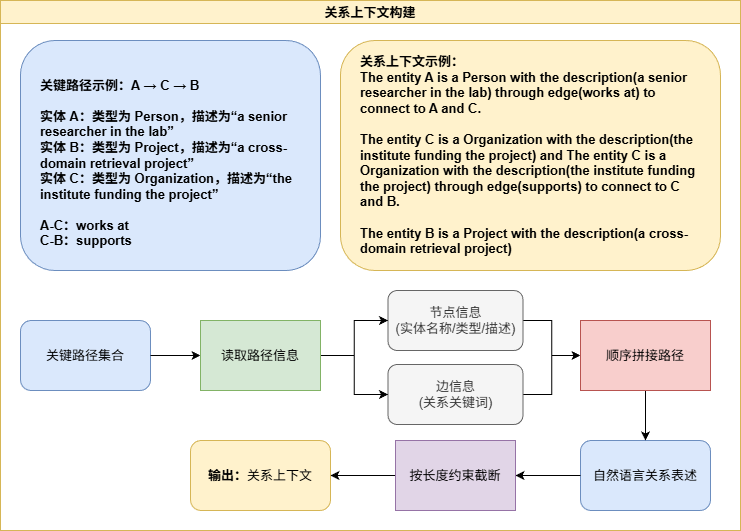
\includegraphics[width=\textwidth]{pic/4picd.png}
\caption{路径提示增强示意图}
    \label{fig:path_prompt}
\end{figure}

\subsection{实体与文本块上下文优化} 
在实体上下文构建方面,本文首先计算实体嵌入 $h_{E}$ 与查询嵌入 $h_{q}$ 的语义相似度,并据此对实体描述进行降序重排。随后,针对超出上下文窗口约束的冗余内容执行长度截断,并统一格式化为实体上下文 $C_{ent}$,以保证有限预算下的语义集中度。

在文本块上下文 $C_{chunk}$ 构建方面,为在固定 Token 预算内同时兼顾信息覆盖度与证据密度,本文提出基于共现频率的启发式筛选流程,具体包括以下三个步骤。

(1)候选集扩展:提取关键路径集合 $\mathcal{P}_{K}$ 中节点及其一跳邻居所关联的来源文本块编号,形成候选文本块集合。

(2)共现频率统计:统计每个文本块编号在关联节点集合中的出现频次。出现频率越高,通常意味着该文本块承载了更多跨实体关联信息,语义密度也更高。

优先级排序与截断:首先按照共现频率由高到低排序;其次在频率相同条件下,优先保留与查询相似度更高节点对应的文本块。基于上述规则,本文自高优先级候选中依次选取文本块,直至达到预设预算上限,并将结果格式化为 $C_{chunk}$。

\subsection{多维上下文融合与答案生成}
对于长上下文条件下的小型语言模型,若直接聚合多源关系路径信息,容易造成证据竞争与注意力分散,从而影响最终生成质量。基于此,本文采用“头尾强化”的上下文组织原则,将高优先级信息置于模板两端,以匹配模型对边界位置信息更敏感的记忆特性。

具体而言,增强表示 $C_{augmented}$ 由查询 $q$ 与三类上下文进行结构化融合得到:将用户查询 $q$ 置于模板头部,将重排序后的关系上下文 $C_{rel}$ 置于模板尾部,并将实体上下文 $C_{ent}$ 与文本块上下文 $C_{chunk}$ 组织于中间区域。最终答案 $A$ 由小型语言模型完成推理生成,其形式化表达如下:
$$A = \text{SLM}(q, C_{augmented}) = \text{SLM}(q, [C_{ent}; C_{chunk}; C_{rel}])$$

图\ref{fig:multi_context_fusion}展示了多维上下文融合流程。图中不同颜色模块对应不同类型的上下文信息,并通过统一模板进行结构化编排与输入,从而在有限预算内提升关键信息利用率与答案生成质量。

\begin{figure}[htb]
    \centering
    \includegraphics[width=\textwidth]{pic/4pic_context.png}
\caption{多维上下文融合示意图}
    \label{fig:multi_context_fusion}
\end{figure}

\section{实验结果分析}
\subsection{数据集介绍}
针对本地私有化与资源受限单机环境下图检索增强生成系统的评估需求,本节选取 LiHua-World 与 MultiHop-RAG 两类具有代表性的数据集开展实验,分别用于考察方法在本地时序场景与跨文档多跳推理场景中的适用性。为避免训练阶段带来的额外变量,本章所有实验均采用零样本推理设置,不对生成模型或嵌入模型进行额外微调。

LiHua-World 数据集主要由长时间跨度的个人聊天记录构成,具有内容碎片化、语境频繁切换以及线上交流与线下事件相互交织等典型端侧数据特征。该数据集在时间维度上保持连续,能够显式体现实体状态、人物关系以及事件演化过程的动态变化,因而适合评估检索方法对时序关系、人物交互链路以及长尾细节信息的建模能力。
实验中使用该数据集的 442 篇聊天记录文档构建图索引,并基于数据集提供的问题-答案对进行评测。

MultiHop-RAG 数据集是一个专门用于评估检索增强生成(RAG)系统在多跳查询任务中性能的基准数据集。该数据集包含 2556 个多跳查询问题。数据集的知识库由英文新闻文章构成,涵盖娱乐、商业、技术等多个领域,确保了内容的多样性和复杂性。该数据集还提供用于支撑检索的 corpus 子集,共包含 609 条语料文本。
根据查询所需的推理类型,数据集将问题分为四种类别:(1)推理查询,需要从多个证据中综合推理得出答案;(2)比较查询,需要对比多个证据中的事实信息;(3)时序查询,需要分析证据的时间顺序和因果关系;(4)空查询,答案无法从证据中得出,用于评估模型在缺乏相关证据时的表现。

\subsection{评测指标及实验设置}
本节从端到端问答效果层面对各类方法进行评估。
端到端问答效果采用准确率(Accuracy, acc)与错误率(Error Rate, err)两个指标作为主比较口径。
其中,准确率表示模型生成答案与标准答案在语义上保持一致的问题比例;错误率表示模型输出存在明显事实错误或关键结论错误的问题比例。这样的设置主要是为了与已有基线工作\cite{edge2024local,guo2024lightrag,fan2024minirag}中常见的主结果报告方式保持一致,从而保证横向比较的可比性。

与第三章保持一致,本文采用 DeepSeek-V3.2\cite{liu2025deepseek} 作为自动化评审模型,在固定提示词与确定性生成配置(temperature = 0)下,将回答判定为一致、错误或拒绝/无关三类。
DeepSeek-V3.2 在本章中仅承担统一评测器的角色,用于对各方法生成答案与标准答案之间的一致性进行自动判定,并不参与任何方法的索引构建、检索或答案生成过程。采用单一强模型作为统一裁判,与近期工作\cite{edge2024local,guo2024lightrag,fan2024minirag}中使用 GPT-4o-mini 等模型进行 LLM-based evaluation 的做法一致。

本文在主结果对比中沿用第三章的下游问答验证实验中的 acc 与 err 作为核心指标。
对于被判定为拒绝或无关的输出,本文既不计入 acc,也不计入 err。
acc 越高、err 越低,说明检索结果对后续答案生成的支撑效果越好。

在结果标注方面,LiHua-World 与 MultiHop-RAG 均采用数据集提供的标准答案作为参考,并统一交由 DeepSeek-V3.2 自动评审模型进行语义一致性判定。
由于本文全部基线方法与所提方法均共享同一评审器、同一提示模板、同一输入格式与同一确定性参数配置,裁判模型可能存在的系统性偏好会在各方法之间被尽可能保持一致,从而使 acc、err更适合作为相对比较指标。

实验设置方面,所有方法均采用统一的文本切分策略,将输入文档切分为长度为 1200 tokens 的文本块,相邻块之间设置 100 tokens 的重叠。
向量检索层统一使用 NanoVectorDB 进行存储与召回。

在 Semantic-Flow RAG 中,检索起点映射阶段分别取前 $N=15$ 个起点节点与前 $M=5$ 个候选答案类型节点,衰减因子$\alpha$ 为0.8,早停阈值 $\theta$ 为0.3,路径筛选阶段保留前 $P=6$ 条关键路径,输入 Token 预算上限8192。

为保证对比公平,NaiveRAG、GraphRAG、LightRAG 与 MiniRAG 均在相同文本分块、相同语言模型骨干以及相同 Token 预算约束下运行。
需要指出的是,对于 GraphRAG 与 LightRAG 等原始设计更偏向社区摘要或全局检索的方法,统一预算会压缩其最优工作区间,因此本章比较结果应理解为在统一小模型与统一资源约束下的相对表现。

在模型配置方面,本章主要以小型语言模型作为生成骨干,并选取 Phi-4-mini-Instruct、Qwen3-4B-Instruct 与 MiniCPM4-0.5B 三种代表性模型进行实验。其中,嵌入模型统一采用 all-MiniLM-L6-v2\cite{reimers2019sentence},以保证不同检索框架之间的差异主要来源于检索机制本身,而非额外的模型规模差异。各基线方法的超参数设置与第三章实验保持一致,后文消融实验覆盖与主结果表一致的三种基础模型。

\subsection{对比实验}
为验证本文方法的整体有效性,本章将 Semantic-Flow RAG 与四类代表性基线方法进行比较,分别为 NaiveRAG、GraphRAG、LightRAG 与 MiniRAG。

(1)NaiveRAG\cite{lewis2020retrieval}:该方法主要用于从文本数据库中进行信息检索,其核心流程为将文本切分为多个文本块并进行存储。在存储过程中,通过文本嵌入技术将这些文本块转换为向量表示。对于给定的查询,首先将查询问题转换为文本嵌入向量,随后基于查询向量与文本块向量之间的最大相似度执行检索操作,进而实现对目标答案的高效、直接获取。

(2)GraphRAG\cite{edge2024local}:作为一种基于图结构的检索增强生成(Retrieval-Augmented Generation, RAG)方法,该方法利用LLM从文本中提取实体和关系,并将其分别表示为图中的节点和边。在本节的实验中使用本地模式,因为全局搜索模式的成本过高。由于 GraphRAG 的检索流程与其社区摘要式索引组织强耦合,本文保留其原始图索引构建方式与原生检索范式,用于作为经典 GraphRAG 在当前统一小模型约束下的端到端系统参照。

(3)LightRAG\cite{guo2024lightrag}:该方法同样属于基于图结构的RAG方法,采用局部与全局相结合的双层检索框架,在图结构中同时从局部和全局两个层面执行更细致、更精准的检索操作,以降低令牌消耗和时间成本。在本章实验中,为尽可能隔离“检索方法”本身带来的差异,LightRAG 不再单独重建图索引,而是与 MiniRAG、Semantic-Flow RAG 共用由 MiniRAG 流程生成的图索引,仅在查询时使用其自身的检索与上下文组织策略。

(4)MiniRAG\cite{fan2024minirag}:面向小模型场景构建轻量图索引与路径辅助检索机制,能够一定程度上缓解大模型依赖问题,因而是本文最具直接参考意义的图基基线方法。在本章中,MiniRAG 既提供共享图索引的构建方式,也作为其原生检索方法的对照。

需指出的是,本章的图基方法对比采用两类索引口径并行设置,对应两类不同结论。其一,GraphRAG 保持原始索引构建与原生检索流程,用于反映经典 GraphRAG 系统在当前统一小模型与统一资源约束下的端到端整体表现。其二,LightRAG、MiniRAG 与 Semantic-Flow RAG 统一采用与 MiniRAG 相同的图索引构建方法,但在检索阶段分别使用各自的方法。因而,前一类结果更适合用于比较不同方案在整体系统层面的综合表现;后一类结果则更适合用于分析共享索引前提下检索起点定位、路径筛选与上下文组织策略带来的差异。

如表\ref{tab:semantic_flow_compare}所示,在统一分块方式与统一 Token 预算约束下,Semantic-Flow RAG 在所报告设定中整体表现出更优的准确率趋势,同时保持了较低的错误率。本文在主结果表中仍以 acc 与 err 作为核心比较依据,以与已有基线工作保持一致;拒答率则作为补充分析指标,用于辅助观察不同方法是否通过增加拒答来换取表面上的准确率提升。需要指出的是,由于不同基线工作对第三类响应的定义可能并不一致,例如有的方法引入部分正确类别,也有的方法将拒绝回答直接计入错误响应,因此 refuse 指标并不具备与 acc、err 相同程度的跨方法可比性。表\ref{tab:semantic_flow_compare}对齐了数据集、分块方式、骨干模型、嵌入模型与 Token 预算,因此可用于比较各方法在统一资源约束下的端到端综合表现。其中,对于 LightRAG、MiniRAG 与 Semantic-Flow RAG 这三种共享 MiniRAG 图索引的方案,其差异可以更集中地解释为检索起点定位、路径筛选与上下文组织策略的差异;而 GraphRAG 由于保留了原始索引构建方式,更适合作为经典系统在当前约束下的整体参照。相对地,本章后续消融实验是在 Semantic-Flow RAG 框架内部逐步移除模块,其结论更适合用于说明起点映射、流式剪枝与路径提示增强各组件的独立作用。

\begin{table*}[htb]
\centering
\caption{Semantic-Flow RAG 与各基线方法在不同骨干模型上的对比实验结果}
\label{tab:semantic_flow_compare}
\setlength{\tabcolsep}{2.6pt}
\small
\begin{tabular*}{\textwidth}{@{\extracolsep{\fill}}ll|ccc|ccc}
\toprule
\textbf{模型} & \textbf{方法} & \multicolumn{3}{c|}{\textbf{LiHua-World}} & \multicolumn{3}{c}{\textbf{MultiHop-RAG}} \\
\cmidrule(lr){3-5} \cmidrule(lr){6-8}
 &  & \textit{acc}(\%) & \textit{err}(\%) & \textit{refuse}(\%) & \textit{acc}(\%) & \textit{err}(\%) & \textit{refuse}(\%) \\
\midrule
\multirow{5}{*}{Phi-4-mini-Instruct}
& NaiveRAG          & 49.76 & 46.62 & 3.62 & 45.20 & 50.55 & 4.25 \\
& GraphRAG          & / & / & / & / & / & / \\
& LightRAG          & 46.31 & 37.52 & 16.17 & 42.50 & 42.80 & 14.70 \\
& MiniRAG           & 61.85 & 36.42 & 1.73 & 54.16 & 42.23 & 3.61 \\
& Semantic-Flow RAG & \textbf{66.80} & \textbf{31.40} & \textbf{1.80} & \textbf{58.90} & \textbf{38.10} & \textbf{3.00} \\
\midrule
\multirow{5}{*}{MiniCPM4-0.5B}
& NaiveRAG          & 47.57 & 48.82 & 3.61 & 42.86 & 52.59 & 4.55 \\
& GraphRAG          & / & / & / & / & / & / \\
& LightRAG          & 44.80 & 38.70 & 16.50 & / & / & / \\
& MiniRAG           & 58.40 & 39.72 & 1.88 & 50.86 & 44.90 & 4.24 \\
& Semantic-Flow RAG & \textbf{63.20} & \textbf{34.70} & \textbf{2.10} & \textbf{55.10} & \textbf{40.80} & \textbf{4.10} \\
\midrule
\multirow{5}{*}{Qwen3-4B-Instruct}
& NaiveRAG          & 53.53 & 42.23 & 4.24 & 49.00 & 47.10 & 3.90 \\
& GraphRAG          & / & / & / & / & / & / \\
& LightRAG          & 48.20 & 35.80 & 16.00 & 45.30 & 40.50 & 14.20 \\
& MiniRAG           & 65.78 & 32.81 & 1.41 & 58.40 & 38.93 & 2.67 \\
& Semantic-Flow RAG & \textbf{71.20} & \textbf{27.60} & \textbf{1.20} & \textbf{63.40} & \textbf{33.80} & \textbf{2.80} \\
\midrule
\multirow{5}{*}{GLM-4.5-Air}
& NaiveRAG          & 65.89 & 40.19 & 0.92 & 61.96 & 24.11 & 13.93 \\
& GraphRAG          & 60.40 & 38.50 & 1.10 & 63.10 & 22.90 & 14.00 \\
& LightRAG          & 68.92 & 29.20 & 1.88 & 59.03 & 27.52 & 13.45 \\
& MiniRAG           & 68.13 & 29.98 & 1.89 & 62.01 & 24.22 & 13.77 \\
& Semantic-Flow RAG & \textbf{73.40} & \textbf{25.60} & \textbf{1.00} & \textbf{67.10} & \textbf{20.10} & \textbf{12.80} \\
\bottomrule
\end{tabular*}
\end{table*}

从表\ref{tab:semantic_flow_compare}可以看出,在当前统一小模型与统一资源约束下,Semantic-Flow RAG 在已获得有效结果的设定中表现出更优的端到端综合性能,准确率整体更高,错误率整体更低,体现出较好的跨模型稳定性。
其中,在 LiHua-World 数据集上,Semantic-Flow RAG 相较于面向 SLM 设计的 MiniRAG 的准确率增益分别达到 4.95、4.80、5.42 与 5.27 个百分点;在更强调跨文档证据整合的 MultiHop-RAG 数据集上,该增益进一步保持在 4.50--5.09 个百分点区间。与此同时,其错误率相较 MiniRAG 也在对应设定下同步下降。由于 MiniRAG、LightRAG 与 Semantic-Flow RAG 共享图索引,这一结果更直接地说明,在共享索引前提下,本文方案在检索信噪比控制与证据组织方式上具有优势。

观察不同基线方法的差异可以发现,NaiveRAG 在两个数据集上的表现整体弱于适配较好的图基方法,说明仅依赖文本块相似度检索难以稳定处理复杂实体关系与多跳推理问题。GraphRAG 则在三种小模型设定下未获得有效结果,仅在 GLM-4.5-Air 这一较强骨干下恢复基本可用性,这与其原始流程对高质量实体关系抽取、社区摘要生成与全局语义整合能力的强依赖是一致的;当骨干模型退化为小模型后,图索引质量与后续上下文摘要质量可能同时失稳,从而使端到端问答流程难以稳定地产生有效回答。

相比之下,LightRAG 虽然在部分设定下仍能运行,但其检索结果通常需要同时携带局部邻域与较高层语义信息,在统一 Token 预算下更容易引入与当前推理路径无关的邻居噪声,因此在共享索引设定下整体表现弱于本文方法。MiniRAG 作为面向小模型场景设计的强基线,整体表现已显著优于 NaiveRAG 与 LightRAG,说明“轻量图索引+路径辅助检索”的技术路线在 SLM 场景中是有效的;而与 MiniRAG 的对比则进一步表明,在相同索引基础上加入更细粒度的边语义筛选与路径级上下文重排后,能够进一步提升复杂多跳问题中的证据利用效率。

结合 refuse rate 可以发现,Semantic-Flow RAG 在获得更高准确率的同时并未通过显著增加拒答来换取表面优势,其拒答比例整体保持在较低水平;尤其在三种小模型设定下,其 refuse rate 与 MiniRAG 基本处于同一量级,但 acc 仍有稳定提升。这说明主结果表所体现的收益并非主要来自更保守的回答策略,而是来自整体检索增强方案对检索信噪比与证据组织方式的优化;至于起点映射、流式剪枝与路径提示增强三类模块的独立贡献,仍需以后文统一框架下的消融实验作为更直接的归因依据。


为进一步验证 Semantic-Flow RAG 方法的行为差异,本节在表\ref{tab:case_analysis}中对比了本文方法与两种基线方法在 LiHua-World 数据集中 3 个代表性样例上的表现。这里的案例分析仅用于定性说明不同检索机制的差异,不作为总体性能结论的唯一依据。
\begin{table}[htb]
\centering
\caption{LiHua-World 数据集中的案例对比结果}
\label{tab:case_analysis}
\small
\renewcommand{\arraystretch}{1.2}
\setlength{\tabcolsep}{2pt}
\begin{tabular}{>{\raggedright\arraybackslash}p{2.15cm}|>{\raggedright\arraybackslash}p{3.35cm}|>{\raggedright\arraybackslash}p{3.35cm}|>{\raggedright\arraybackslash}p{3.35cm}}
\hline
 & \centering\arraybackslash\textbf{Case 1} & \centering\arraybackslash\textbf{Case 2} & \centering\arraybackslash\textbf{Case 3} \\
\hline
\textbf{Question} &
Did Turalyon announce the construction updates and feedback from residents after Illidan Stormrage complained about the construction noise? &
Who wished Li Hua a happy Lunar New Year? &
What is the name of the Italian restaurant where Wolfgang and Li Hua are having dinner to celebrate Wolfgang's promotion? \\
\hline
\textbf{Gold answer} &
\textbf{Yes} &
\textbf{Adam Smith \& Jennifer Moore \& Wolfgang Schulz} &
\textbf{Venedia Grancaffe} \\
\hline
\textbf{LightRAG} &
No, Turalyon did not announce construction updates or feedback from residents after the complaint. &
Adam Smith \& Wolfgang Schulz &
\textbf{Venedia Grancaffe} \\
\hline
\textbf{MiniRAG} &
No, Turalyon did not announce construction updates or feedback from residents after the complaint. &
\textbf{Adam Smith \& Jennifer Moore \& Wolfgang Schulz} &
The restaurant name is not explicitly stated in the provided data. \\
\hline
\textbf{Semantic-Flow RAG} &
\textbf{Yes}, Turalyon announced construction updates and incorporated resident feedback after the complaint. &
\textbf{Adam Smith \& Jennifer Moore \& Wolfgang Schulz} &
\textbf{Venedia Grancaffe} \\
\hline
\end{tabular}
\end{table}

从表\ref{tab:case_analysis}可以看出,三种方法在不同类型的查询场景中呈现出显著的性能差异。

案例一的查询问题涉及多跳推理与因果关系理解。LightRAG与MiniRAG均给出错误答案“No”,而Semantic-Flow RAG能够正确推断出“Yes”。这种性能差异主要源于三种方法在检索机制上的根本区别。具体而言,LightRAG采用节点及其一跳邻居的检索策略,虽然能够获取局部上下文信息,但当问题涉及跨越多个节点的因果链时(如“投诉→应对措施→反馈”的三跳关系),简单的一跳邻居检索难以捕捉完整的因果链条。MiniRAG尽管构建了轻量图索引,但其检索过程仍然受限于局部信息聚合能力,且在处理时序性因果关系时缺乏显式的路径引导机制。相比之下,Semantic-Flow RAG通过查询语义引导的起点映射机制,首先从问题中提取关键实体(Turalyon、Illidan Stormrage),然后利用融合边语义权重的自适应流式剪枝算法,在图索引中精准定位连接“投诉”与“施工更新”的关键推理路径。这种基于路径的检索方式不仅跨越了多跳关系,还保留了每一步推理的语义关联,使得小型语言模型能够在结构化提示的引导下完成复杂的因果推理。

案例二的查询问题聚焦于实体枚举与完整性校验。MiniRAG与Semantic-Flow RAG均能够完整召回三个实体(Adam Smith、Jennifer Moore、Wolfgang Schulz),而LightRAG遗漏了Jennifer Moore。这一现象体现了不同方法在实体覆盖度上的差异。LightRAG基于查询向量的相似度匹配进行节点召回,当不同实体与查询的语义相似度存在差异时,容易召回不完整的结果集。MiniRAG通过轻量图索引结构化组织实体关系,能够在一定程度上缓解召回不完整的问题,但其字符串级去重策略在面对同义异形的实体指代时仍可能产生冗余节点,影响检索精度。Semantic-Flow RAG在继承图索引结构化优势的基础上,通过起点映射阶段对查询进行实体提取和答案类型预测,预先锁定了答案空间,从而在检索阶段能够更有针对性地遍历所有潜在答案节点。此外,该方法采用的多锚点路径检索策略能够从多个起点并行探索图结构,进一步提升了实体枚举的完整性。

案例三的查询问题属于事实性信息提取与精确匹配。LightRAG与Semantic-Flow RAG均能准确提取餐厅名称“Venedia Grancaffe”,而MiniRAG则给出“数据中未明确说明”的错误回答。这种差异凸显了精确匹配任务中对检索粒度的不同要求。LightRAG的一跳邻居检索策略在处理简单事实性问题时表现尚可,当餐厅名称作为Wolfgang或Li Hua的直接邻居节点存在时,该方法能够有效召回。然而,MiniRAG在该案例中的失败可能源于两个方面:一是其轻量图索引在构建阶段可能遗漏了部分细粒度关系,二是其检索机制在处理特定类型的查询时缺乏足够的语义引导。Semantic-Flow RAG通过查询语义引导的起点映射,能够准确识别“餐厅名称”这一答案类型,并在流式剪枝阶段优先保留与该类型高度相关的路径节点。同时,该方法基于路径的结构化提示增强机制,将节点和关系按照路径顺序组织,为小型语言模型提供了更强的上下文线索,使其能够在有限的上下文预算内精准定位事实信息。

综上所述,通过上述三个案例可以观察到不同方法在小型语言模型场景下的适用边界存在差异。具体而言,LightRAG 在处理简单事实性查询时具有一定优势,但在涉及复杂多跳推理时表现出明显局限性;MiniRAG 通过轻量图索引提供了基础的结构化知识表示,在实体枚举等中等复杂度任务上表现较好,但在高精度事实提取和复杂推理任务上仍存在不足;Semantic-Flow RAG 在这三个代表性案例中均给出了更完整或更准确的回答。需指出的是,上述案例分析主要用于辅助解释端到端结果中的行为差异,不能单独推出模块层面的因果结论或通用性结论。

\subsection{消融实验}
为进一步揭示Semantic-Flow RAG各组成模块的协同作用机制,本章设计了三组消融实验,并在与主结果表一致的三种基础模型上进行测试。通过逐步移除起点映射、关键路径发现与路径提示增强模块,系统性地考察各组件对最终性能的影响。

(1)变体A(w/o StartMap):移除查询语义引导的检索起点映射机制,仅使用查询整体嵌入直接召回候选节点,旨在验证实体提取与答案类型预测在起点初始化阶段的作用。

(2)变体B(w/o Semantic-Flow):移除融合边语义权重的自适应流式剪枝机制,改为保留锚点对之间的最短跳数路径,旨在验证关键路径发现机制的重要性。

(3)变体C(w/o PathPrompt):保留关键路径检索结果,检索到的路径会被分解为独立的节点和边。节点与边的顺序是随机的,不会基于其原始路径进行结构化组织,旨在验证路径提示增强策略的重要性。

需指出的是,主结果表主要用于说明本文整体方案在统一资源约束下的端到端有效性;而关于起点映射、流式剪枝与路径提示增强三类模块的独立贡献,更直接的证据来自保持统一框架与统一索引条件下的消融实验。如表\ref{tab:semantic_flow_ablation}所示,在 LiHua-World 数据集与三种基础模型上,完整的 Semantic-Flow RAG 在各项指标上均优于所有消融变体,说明三个模块之间存在明确的协同增益。

\begin{table*}[htb]
\centering
\caption{Semantic-Flow RAG 的消融实验结果}
\label{tab:semantic_flow_ablation}
\setlength{\tabcolsep}{2.8pt}
\small
\begin{tabular*}{\textwidth}{@{\extracolsep{\fill}}ccccccccc}
\toprule
\multirow{2}{*}{\textbf{模型}} & \multicolumn{2}{c}{\textbf{Semantic-Flow RAG}} & \multicolumn{2}{c}{\textbf{w/o StartMap}} & \multicolumn{2}{c}{\textbf{w/o Semantic-Flow}} & \multicolumn{2}{c}{\textbf{w/o PathPrompt}} \\
\cmidrule(lr){2-3} \cmidrule(lr){4-5} \cmidrule(lr){6-7} \cmidrule(lr){8-9}
& \textit{acc}(\%) & \textit{err}(\%) & \textit{acc}(\%) & \textit{err}(\%) & \textit{acc}(\%) & \textit{err}(\%) & \textit{acc}(\%) & \textit{err}(\%) \\
\midrule
Phi-4-mini-Instruct & 66.80 & 31.40 & 60.10 & 37.20 & 62.40 & 35.30 & 63.10 & 34.60 \\
MiniCPM4-0.5B & 63.20 & 34.70 & 56.40 & 41.20 & 58.90 & 38.90 & 59.70 & 37.80 \\
Qwen3-4B-Instruct & 71.20 & 27.60 & 64.50 & 33.90 & 66.30 & 31.80 & 67.10 & 30.90 \\
\bottomrule
\end{tabular*}
\end{table*}

消融实验结果表明,检索起点映射机制对整体性能具有基础性作用。移除该模块后,三种模型的准确率分别由 66.80\%、63.20\% 与 71.20\% 降至 60.10\%、56.40\% 与 64.50\%,错误率同步升至 37.20\%、41.20\% 与 33.90\%。该结果说明,对于小型语言模型场景,在检索前通过轻量级语义解析缩小搜索空间,是提升图检索有效性的关键前提。

其次,移除关键路径发现机制后,三种模型的准确率分别降至 62.40\%、58.90\% 与 66.30\%,错误率分别升至 35.30\%、38.90\% 与 31.80\%。虽然系统仍可通过最短路径获得部分结构信息,但由于缺乏边语义权重建模与早停剪枝策略,大量低相关边被保留下来,从而削弱了检索结果的信噪比并带来更高的错误率。这一结果表明,关键路径发现模块并非简单的路径压缩步骤,而是决定检索结果信噪比的核心组成部分。

最后,路径提示增强机制对答案生成阶段同样具有直接影响。移除该机制后,三种模型的准确率分别回落至 63.10\%、59.70\% 与 67.10\%,错误率也分别上升至 34.60\%、37.80\% 与 30.90\%。这一变化趋势与 PathRAG 原始消融实验中“路径化提示优于扁平组织”的结论一致:检索结果虽仍然包含关键实体和关系,但由于节点与边被打散后失去了显式路径结构,模型在生成时更难保持推理链路的连续性,最终表现为准确率下降而错误率上升。由此可见,路径级上下文组织方式不仅影响检索结果的表达形式,也直接影响小型语言模型对关系证据的利用效率。

综上所述,查询语义引导的起点映射、融合边语义权重的自适应流式剪枝以及基于路径的提示增强三类机制共同构成了 Semantic-Flow RAG 的核心能力来源。基于当前消融结果,可以认为三者对最终性能均有正向贡献;但若要进一步证明该结论在更多骨干模型与更多数据集上严格成立,仍需补充更大规模的交叉验证实验。
\section{本章小结}
本章围绕小型语言模型在图检索增强生成阶段所面临的起点定位误差、路径噪声累积以及长上下文组织低效等关键问题展开研究,在前一章高质量图索引构建结果的基础上,提出了查询语义引导与边感知增强的图检索增强生成方法 Semantic-Flow RAG。首先,本章从查询语义解析出发,设计了检索起点映射机制,通过小型语言模型完成关键实体提取与答案类型预测,并结合语义相似度匹配生成更具针对性的锚点集合,从而提升查询与图节点之间的对齐精度。其次,针对传统图检索方法容易保留大量低相关边与无关邻居的问题,本章提出了融合边语义权重的自适应流式剪枝算法,通过资源传播与早停控制在候选路径中动态筛选高价值推理链路,以降低检索结果中的结构化噪声。最后,面向小型语言模型在长序列输入中易出现“中间迷失”的局限性,本章进一步设计了基于路径的提示增强机制,将节点与关系按照原始推理路径进行结构化组织,以保留实体间的逻辑顺序并增强模型对核心证据的关注能力。

在实验验证方面,本章基于 LiHua-World 与 MultiHop-RAG 两类具有代表性的数据集,从端到端问答表现角度系统评估了所提方法的有效性。实验结果表明,在当前统一小模型与统一预算约束的设定下,Semantic-Flow RAG 表现出较好的端到端综合性能。其中,在 Qwen3-4B-Instruct 骨干模型下,该方法在 LiHua-World 上取得了 71.20\% 的准确率、27.60\% 的错误率与 1.20\% 的拒答率,在 MultiHop-RAG 上也表现出较好的问答能力。进一步地,主结果对比说明了本文方案在整体系统层面的有效性,而在 LightRAG、MiniRAG 与 Semantic-Flow RAG 共享图索引的设定下,其结果也更直接地表明本文方案在检索与上下文组织策略上具有优势。消融实验则进一步表明,查询语义引导的起点映射、边感知流式剪枝以及路径提示增强三类机制均对最终性能具有正向贡献,而案例分析从行为层面补充说明了不同方法在典型问题上的表现差异。

综上所述,本章并非通过引入更大规模的模型参数来换取更高的检索效果,而是通过对图检索流程与上下文组织方式进行系统性优化,构建了一套更适配小型语言模型能力边界的图检索增强生成方案。从端到端实验结果看,该方案在统一小模型与统一资源约束下表现出较好的综合性能;而在共享图索引的比较设定下,其检索起点定位、路径筛选与上下文组织优势体现得更为明确。由此,本章不仅为本地私有化与资源受限单机场景下提升图基问答质量与效率提供了可行路径,也为下一章面向实际应用部署的系统设计与实现提供了直接的方法基础。

\chapter{面向小型语言模型的图检索增强生成系统}

随着本地计算能力的提升与数据隐私保护意识的增强,在本地部署小型语言模型以实现智能问答服务已成为当前自然语言处理领域的研究热点。然而,小型语言模型在图基检索增强生成任务中面临着索引构建质量低与检索噪声敏感两大核心挑战,严重制约了其在实际应用场景中的性能表现。前两章分别提出了验证优先的图索引构建方法与查询语义引导的边感知增强检索方法,从理论层面缓解了上述问题,并为构建本地私有化图检索增强生成系统提供了方法基础。

针对本地私有化与资源受限单机部署场景下的实际应用需求,本章基于上述理论方法从系统需求分析出发,对系统总体架构、核心功能模块以及数据库存储方案进行系统性设计。按照既定的设计原则与规范,实现图索引构建、语义检索与答案生成三大核心功能,使系统具备从原始文本摄入到结构化图谱构建再到问答响应的全流程自动化处理能力。最后,通过实际应用场景的系统展示与多维度性能测试,对系统在图基检索增强生成任务中的有效性与实用性进行验证。

\section{系统需求分析}

\subsection{功能需求分析}

对于功能性需求,本系统将整体功能划分为知识图谱构建、智能检索问答以及系统管理监控三个部分。其中,知识图谱构建部分包括数据接入、实体关系抽取、图谱构建与优化等功能;智能检索问答部分包括查询解析、语义检索、路径推理与答案生成等功能;系统管理监控部分则包括图谱可视化、系统监控与配置管理等功能。基于上述分析,SLM-GraphRAG系统主要包含以下三类功能需求:

(1)知识图谱构建:实现从原始文本到结构化知识图谱的自动化构建与维护。该需求涵盖数据接入与预处理、实体关系抽取、图谱去重与优化、向量索引构建等核心功能,以支持构建低冗余度、较高准确性的知识图谱,为后续智能检索提供知识基础。

(2)智能检索问答:实现对用户自然语言查询的语义理解与回答生成。该需求涵盖查询语义分析、检索起点映射、关系路径推理、多跳上下文组织以及答案生成等核心功能,通过验证优先的图索引构建方法与语义引导的边感知增强检索方法,支持在资源受限的单机环境中提供较高质量的问答服务。

(3)可视化界面:提供简洁直观的Web用户界面,降低系统使用门槛并提升用户体验。该需求涵盖智能问答交互、图谱可视化浏览、文档管理、实体管理以及系统监控等功能模块,支持用户通过图形化界面完成从数据上传、索引构建到智能问答的全流程操作。


\begin{figure}[htb]
    \centering
    \includegraphics[width=\textwidth]{pic/5pic_dataflow.png}
\caption{SLM-GraphRAG系统数据流图}
    \label{fig:5dataflow}
\end{figure}

图\ref{fig:5dataflow}展示了SLM-GraphRAG系统的数据流转过程。首先,数据接入模块作为系统与外部数据源的交互入口,负责接收多源异构数据并完成预处理,从而为知识图谱构建提供标准化输入。该模块支持纯文本、Markdown、PDF等多种文档格式,以及JSON、GraphML、CSV等知识图谱格式导入,并通过数据清洗、格式转换与文本分块等操作保证输入数据的一致性与准确性。其次,图谱构建模块承担知识抽取与结构化存储任务,一方面利用验证优先实体关系抽取算法(VF-GIM)从文本中提取实体与关系,构建初步知识图谱结构;另一方面再通过去重、合并与优化算法生成高质量知识图谱,并分别写入图数据库与向量数据库,以为后续语义检索提供索引支撑。最后,智能检索模块作为系统核心处理单元,负责理解用户查询语义、从知识图谱中检索相关路径与上下文,并通过答案生成模块输出结构化问答结果。具体而言,查询理解与映射功能采用查询语义引导的检索起点映射方法定位相关实体与答案类型,知识检索与推理功能利用边感知增强的流式剪枝算法识别关键关系路径并提取多维上下文信息,最终答案生成功能则基于关系路径提示增强策略调用小型语言模型生成具备逻辑性的答案,并为答案标注推理路径与信息来源,从而确保回答的可解释性与可信度。


\subsection{非功能需求分析}

除核心功能需求外,系统还需要满足以下非功能性需求,以确保其在实际部署场景中的可用性与可靠性:

(1)性能需求。考虑到资源受限单机环境的计算资源限制,系统应在保证检索质量的前提下,尽可能降低推理延迟与资源占用。系统应具备处理中等规模数据集的能力,在单台本地设备上支持万级实体的知识图谱构建与秒级响应的查询检索。

(2)可扩展性需求。系统架构应采用模块化设计,各核心组件(如数据接入模块、图谱构建模块、检索模块等)应保持低耦合,便于后续功能扩展或技术升级。系统应支持不同规模的语言模型接入,允许用户根据设备资源与性能需求灵活选择。此外,系统应具备良好的接口规范,便于集成到第三方应用或工作流中。

(3)隐私与安全需求。作为面向本地私有化部署的系统,应支持所有数据处理过程在本地完成,不依赖云端API调用。系统需确保用户数据不外泄,支持完全私有化部署模式。

(4)易用性需求。系统需提供简洁直观的用户界面,包括命令行工具与可选的图形化界面,降低不同技术背景用户的使用门槛。对于知识图谱构建、检索配置等复杂操作,系统应提供合理的默认参数,并支持用户根据具体场景进行灵活调整。

\section{系统设计}

\subsection{架构设计}

SLM-GraphRAG系统采用分层架构设计,其整体架构如图\ref{fig:5archi}所示,共划分为数据层、处理层、检索层与应用层四个层次。
\begin{figure}[htb]
    \centering
    \includegraphics[width=\textwidth]{pic/5pic_archi.png}
\caption{SLM-GraphRAG系统架构图}
    \label{fig:5archi}
\end{figure}

(1)数据层。该层负责多源异构数据的统一存储与管理,包括文档数据库、向量数据库与图数据库三个核心组件。其中,文档数据库用于存储导入的原始文本数据及其元数据;向量数据库用于存储文本块、实体名称与关系描述的向量表示,以支持语义相似度检索;图数据库则用于存储构建得到的知识图谱,包括实体节点、关系边及其属性描述,从而支持高效图遍历与子图查询操作。

(2)处理层。该层承担知识图谱构建的核心逻辑,负责将原始文本转化为结构化知识索引。其包含数据摄入、实体关系抽取与图谱优化三个核心组件,共同完成从非结构化文本到高质量知识图谱的转换过程。

(3)检索层。该层实现查询智能检索功能,负责理解用户查询并从知识图谱中定位相关知识。其包含查询解析、路径检索与上下文组织三个组件,通过语义对齐、流式剪枝与多维上下文融合实现精准的多跳推理检索。

(4)应用层。该层面向终端用户提供交互接口,包括命令行工具与可选Web界面。应用层支持查询问答、索引管理、图谱可视化与系统监控等功能,从而为用户提供较为友好的系统使用体验。

\subsection{核心功能模块设计}

本节详细描述系统的核心功能模块,各模块采用清晰的职责划分与规范的接口设计,共同支撑系统功能的实现。本文将前文提出的两类核心算法深度集成到相应模块中:验证优先图索引构建方法(VF-GIM)集成于索引构建模块；查询语义引导的边感知增强检索方法(Semantic-Flow RAG)集成于智能问答模块。以下详细描述各模块的功能实现,各个核心模块的详细设计如图\ref{fig:5func_archi}所示。
\begin{figure}[htb]
    \centering
    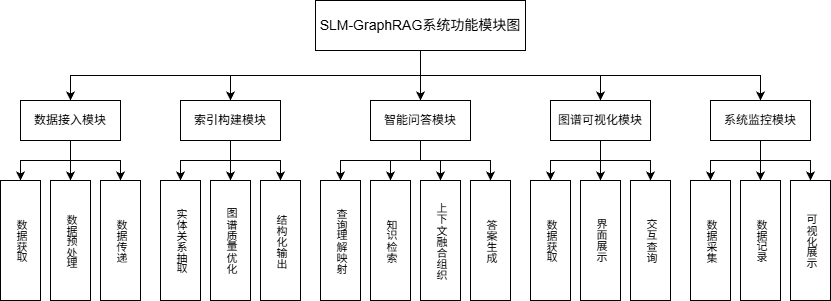
\includegraphics[width=\textwidth]{pic/5pic_func_archi.png}
\caption{SLM-GraphRAG功能模块架构图}
    \label{fig:5func_archi}
\end{figure}


(1)数据接入模块。该模块是整个系统的入口,负责多源异构数据的统一接入与预处理。首先,数据获取功能支持用户上传文档文件(支持纯文本、Markdown、PDF等格式)或外部知识图谱(支持JSON、GraphML、CSV格式),系统对上传的数据类型进行验证,以保证格式正确且完整。其次,数据预处理功能根据需求对数据进行清洗、格式转换与标准化处理,包括文件类型转换、数据去重、分块等操作,从而保证数据的一致性和准确性。最后,数据传递功能将处理后的标准化文本块(包含唯一标识符与元数据)传递至索引构建模块,为后续的知识图谱构建提供输入。此外,该模块支持增量更新与灵活的分块配置选项,以适应不同规模的数据接入需求。该模块工作流程如图\ref{fig:5data_ingest}所示。
\begin{figure}[htb]
    \centering
    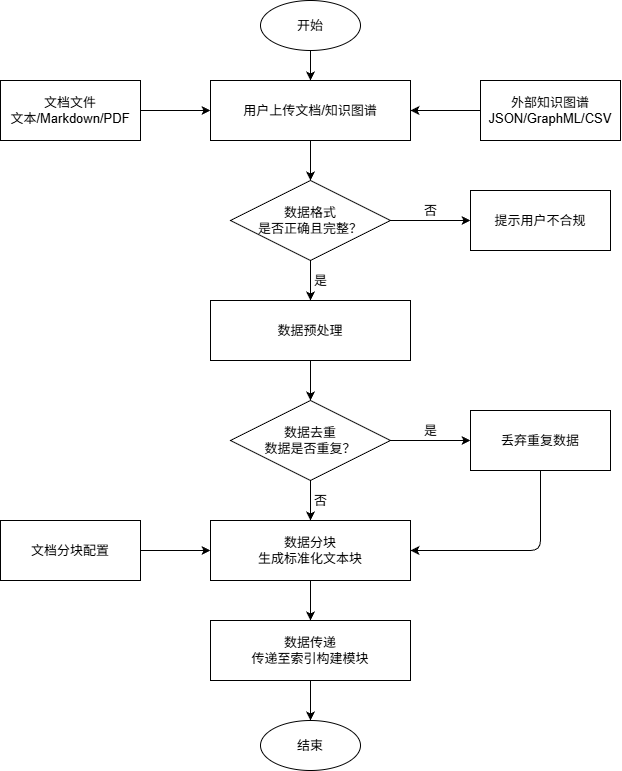
\includegraphics[width=\textwidth]{pic/5pic数据接入模块.png}
\caption{SLM-GraphRAG数据接入模块流程图}
    \label{fig:5data_ingest}
\end{figure}

(2)索引构建模块。该模块是系统的核心处理单元之一,负责从非结构化文本中自动构建结构化知识图谱,实现本文第三章提出的验证优先图索引构建方法。首先,实体关系抽取功能利用前文第三章中设计的验证优先图索引构建方法,从文本中自动抽取实体与关系,构建初步的知识图谱结构。其次,图谱质量优化功能通过图数据去重合并优化算法对初步构建的图谱进行质量优化,生成低冗余、较高纯净度的知识图谱。最后,结构化输出功能将优化后的知识图谱转换为包含实体节点、关系边及其属性描述的结构化格式,为后续的智能检索提供数据支撑。该模块支持增量式更新、实体消歧与类型统一等关键特性,以提升知识图谱的可用性与一致性。该模块工作流程如图\ref{fig:5index_build}所示。
\begin{figure}[htb]
    \centering
    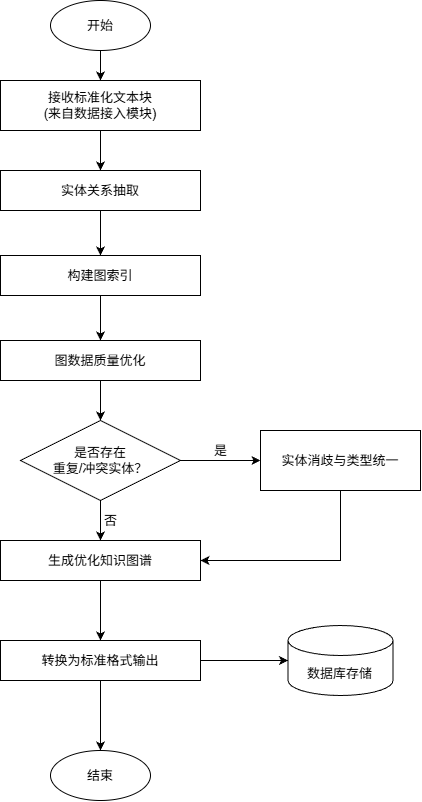
\includegraphics[width=\textwidth]{pic/5pic索引构建模块.png}
\caption{SLM-GraphRAG索引构建模块流程图}
    \label{fig:5index_build}
\end{figure}

(3)智能问答模块。该模块是系统实现智能问答的核心,负责理解用户查询、从知识图谱中检索相关知识并生成答案,实现本文第四章提出的查询语义引导的边感知增强检索方法(Semantic-Flow RAG)。首先,查询理解与映射功能接收用户的自然语言查询,利用前文第四章中设计的查询语义引导检索起点映射方法,从知识图谱中定位相关的检索起点。其次,知识检索与推理功能采用边感知增强的流式剪枝算法,识别关键关系路径并提取多维上下文信息,包括实体上下文、文本块上下文和关系上下文。再次,上下文融合与组织功能对检索到的多维上下文信息进行截断与整合,将关键关系路径与上下文进行结构化组织。最后,答案生成与标注功能调用语言模型,利用前文第四章中设计的基于关系路径的提示增强方法生成答案,该方法能够保留推理链路结构,生成具有一定逻辑性的回答,同时为答案标注推理路径与信息来源,以提升答案的可解释性与可信度。该模块能够为用户提供可追溯的智能问答服务,其工作流程如图\ref{fig:5smart_qa}所示。
\begin{figure}[htb]
    \centering
    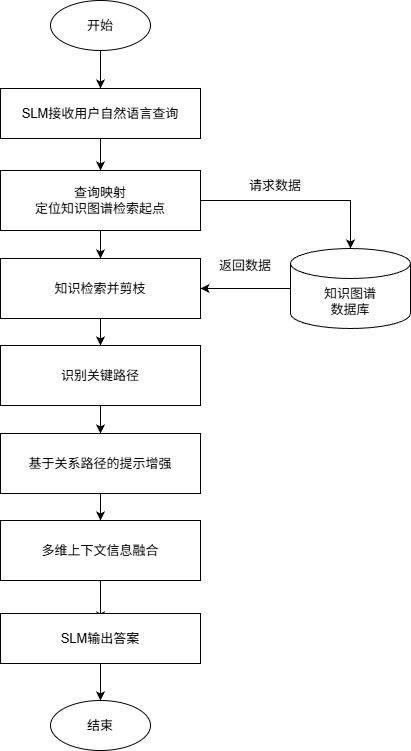
\includegraphics[width=\textwidth]{pic/5pic智能问答模块.png}
\caption{SLM-GraphRAG智能问答模块流程图}
    \label{fig:5smart_qa}
\end{figure}

(4)图谱可视化模块。该模块负责将系统中的知识图谱数据通过图形化界面展示给用户,提供直观的浏览与检索功能。首先,数据获取功能从知识图谱中提取相关数据,包括实体类型、实体描述、关系信息等。其次,界面展示功能将获取到的数据通过分类列表、关系网络图等形式展现给用户,把抽象的图谱数据转化为直观的可视化元素,用户能够一目了然地浏览实体类别、搜索特定实体并查看详情。最后,交互查询功能支持类型驱动的分类展示与语义相似度搜索,用户可以根据实体类型进行分类浏览,或通过关键词进行模糊搜索,快速定位目标实体。该模块还提供关联关系可视化功能,以图形化方式展示实体间的关系网络,帮助用户更好地理解知识图谱的结构与内容。该模块工作流程如图\ref{fig:5graph_vis}所示。
\begin{figure}[htb]
    \centering
    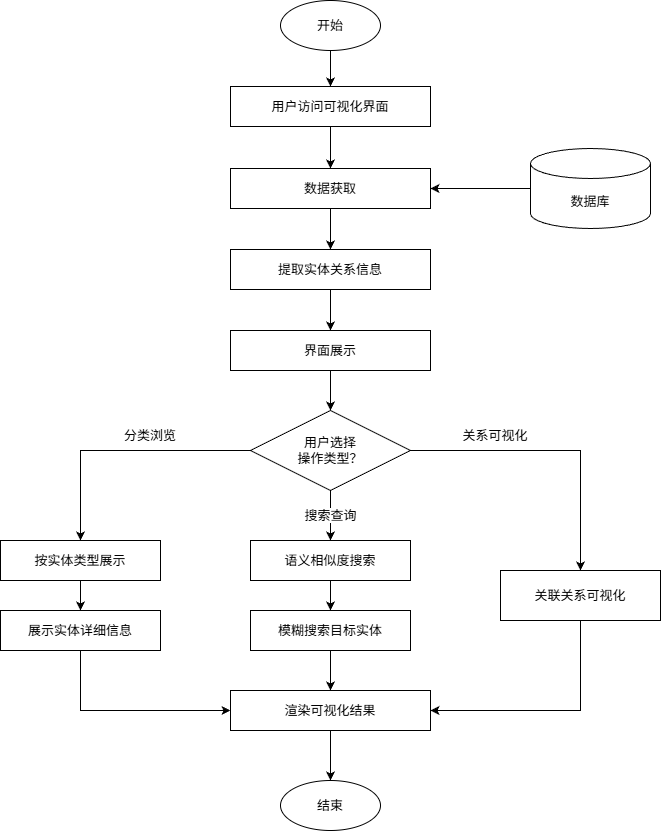
\includegraphics[width=\textwidth]{pic/5pic可视化模块.png}
\caption{SLM-GraphRAG可视化模块流程图}
    \label{fig:5graph_vis}
\end{figure}

(5)系统监控模块。该模块负责系统运行状态的实时监控与分析,以支持系统稳定运行与性能优化。首先,数据采集功能从系统运行时采集各类核心指标数据,包括图谱规模统计(节点数、边数等)、查询总量统计、内存与显存占用监控以及系统健康状态评估(运行状态、异常信息等)。其次,数据记录功能将采集的数据记录到日志文件中,便于后续分析与审计。最后,可视化展示功能通过指标卡片与日志面板集中展示关键运行信息,帮助管理员快速掌握当前系统状态。通过实时监控与日志追踪,该模块能够帮助发现潜在问题、优化系统性能,并为系统维护与升级提供数据支持。

该模块工作流程如图\ref{fig:5system_monitor}所示。
\begin{figure}[htb]
    \centering
    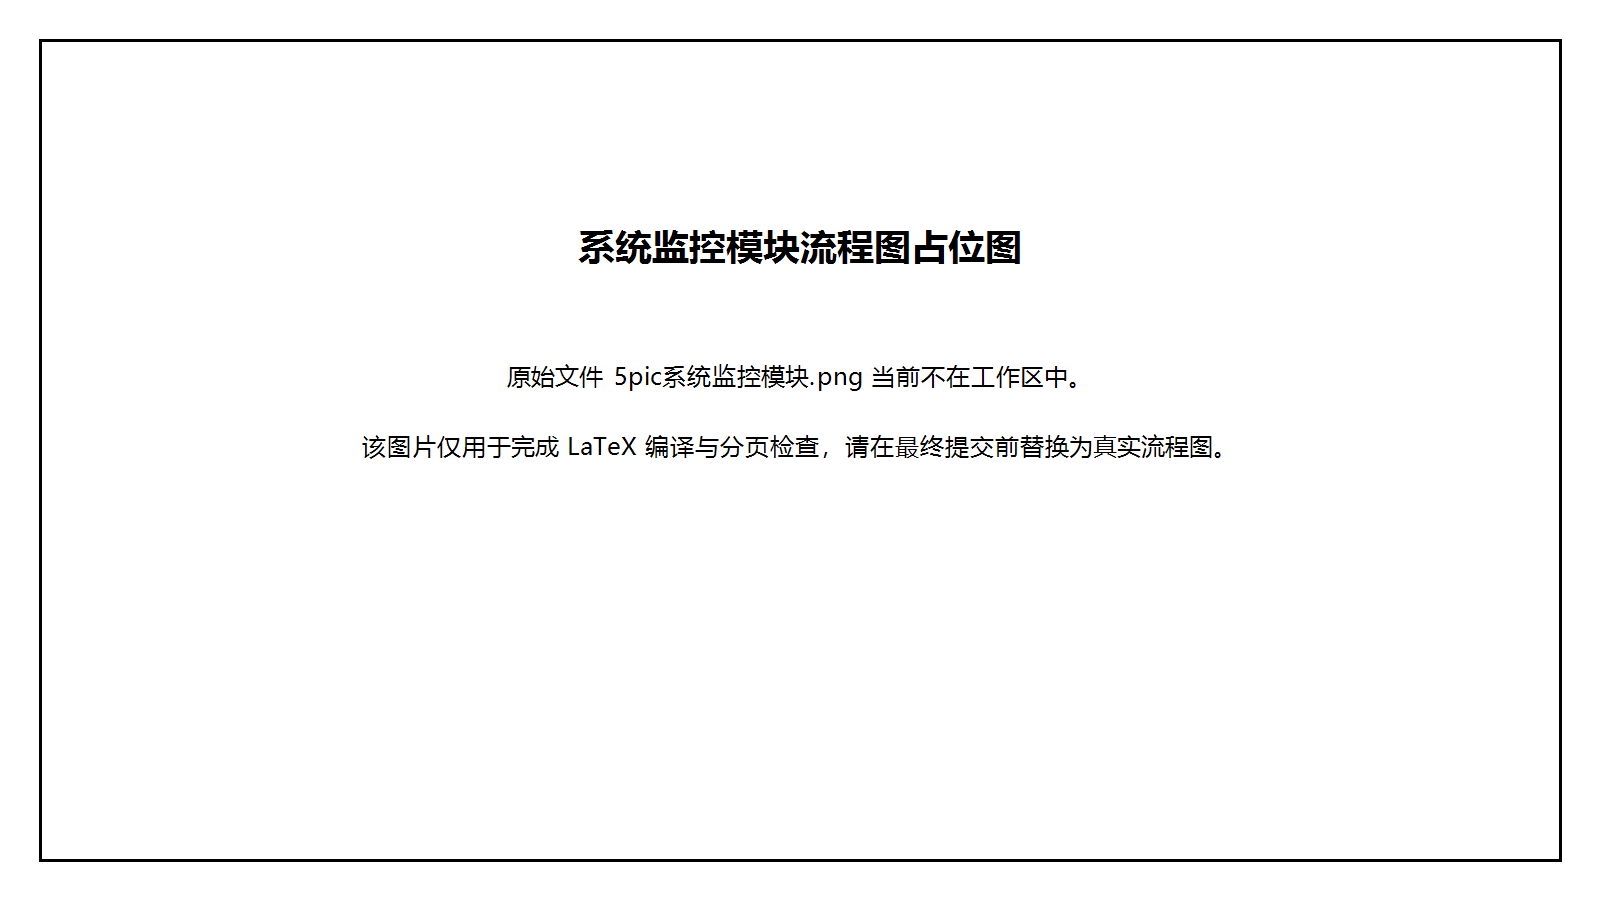
\includegraphics[width=\textwidth]{pic/5pic系统监控模块.png}
\caption{SLM-GraphRAG系统监控模块流程图}
    \label{fig:5system_monitor}
\end{figure}

\subsection{数据库设计}

用户输入的原始文本数据需要经过入队、分块、实体抽取等多个处理阶段,各阶段的中间结果与最终结果均需持久化以供后续检索与分析使用。系统采用多后端可插拔的存储架构,通过JSON文件、NetworkX图、NanoVectorDB向量库等多种存储驱动,整体数据存储平台涵盖文档状态信息、完整文档内容、文本分块、知识图谱、向量索引以及LLM响应缓存六类数据,具体设计如下:

(1)图数据库设计。如表\ref{tab:graph_db}所示,系统使用 NetworkX 图计算库存储知识图谱,定期持久化为 GraphML 格式文件,其中命名空间为 chunk\_entity\_relation。NetworkX 是一个纯 Python 图计算库,支持高效的图遍历与子图查询操作,无需部署外部数据库服务,适合本地私有化与轻量级单机场景。
每个节点代表从文本中抽取的实体,节点标识符为大写规范化的实体名称。节点属性包含:实体类型,如人物、地点、概念等、实体的语义描述与来源分块ID。当关系抽取过程中发现未知实体时,系统会自动创建 entity\_type 为 “UNKNOWN” 的占位节点,确保图的完整性。

每条边连接两个相关实体,记录它们之间的关系类型。边属性包含:src\_id(源实体标识)、tgt\_id(目标实体标识)、relation\_type(关系类型的简短关键词,通过 edge\_keywords 字段存储)、description(关系的详细语义描述)与 source\_id(来源分块ID)。

该图由实体抽取流程动态构建,在查询模式中,系统通过图遍历(获取邻居节点与关联边)来扩展检索上下文,是系统区别于朴素RAG的核心数据结构。该设计支持高效的图遍历与子图查询操作。

\begin{table}[htb]
\caption{图存储设计说明}
\centering
\setlength{\tabcolsep}{2pt}
\begin{tabular}{@{}>{\raggedright\arraybackslash}p{1.6cm}>{\raggedright\arraybackslash}p{1.8cm}>{\raggedright\arraybackslash}p{1.9cm}>{\raggedright\arraybackslash}p{1.9cm}>{\raggedright\arraybackslash}p{4.4cm}@{}}
\toprule
存储对象 & 字段名 & 数据类型 & 约束 & 描述 \\
\midrule
节点(实体) & node\_id        & VARCHAR  & Primary Key & 实体唯一标识(大写规范化) \\
             & entity\_type    & VARCHAR  & Not Null    & 实体类型(如人物、地点、概念等) \\
             & description     & TEXT     & Not Null    & 实体语义描述 \\
             & source\_id      & VARCHAR  & Not Null    & 来源分块ID \\
\midrule
边(关系)   & src\_id         & VARCHAR  & Not Null    & 源实体ID \\
             & tgt\_id         & VARCHAR  & Not Null    & 目标实体ID \\
             & \shortstack[l]{relation\_\\type}  & VARCHAR  & Not Null    & 关系类型的简短关键词 \\
             & description     & TEXT     & Not Null    & 关系语义描述 \\
             & source\_id      & VARCHAR  & Not Null    & 来源分块ID \\
\bottomrule
\end{tabular}
\label{tab:graph_db}
\end{table}

(2)向量数据库设计。如表\ref{tab:vector_db}所示,系统采用nano-vectordb向量库构建向量索引。nano-vectordb是一个极轻量的纯Python向量数据库库,在内存中执行余弦相似度检索,并定期持久化为本地文件,适合本地私有化与轻量级单机场景。
向量存储层共包含四类向量:
实体向量表(命名空间:entities)存储从文本中抽取的实体及其语义描述的向量表示。该表将实体名称与描述拼接后进行向量化,并附带元字段 entity\_name 用于原始实体名追溯,支持语义级实体召回。在本地检索模式中,系统通过该表定位与查询语义最相关的前 K 个实体节点,并结合知识图谱扩展其邻居节点,构建局部上下文。

实体名向量表(命名空间:entities\_name)专门对实体名称进行轻量级向量化,仅存储实体名称本身的向量表示,附带元字段 entity\_name。该表用于候选实体的快速精确召回,作为实体向量表的补充,能够在实体名称明确或需要精确匹配的场景下提供高效检索。

关系向量表(命名空间:relationships)存储实体间关系描述的向量表示,附带 src\_id(源实体标识)与 tgt\_id(目标实体标识)两个元字段,用于追溯关系的参与实体。该表将关系的关键词描述进行向量化,供全局检索模式检索关系上下文。系统通过该表定位与查询相关的前 K 条关系边,进而遍历关系所连接的实体社区,构建全局上下文,支持跨文档的关联推理。

分块向量表(命名空间:chunks)存储所有文本分块的向量表示,是朴素检索模式的核心数据源。该表对文档切分后的每个文本块进行向量化,无需额外元字段。当查询不需要复杂的图遍历时,系统可直接通过该表执行传统的文档片段检索,返回与查询最相关的前 K 个文本块。

每个向量条目关联原始文本ID与元数据,支持快速的相似度搜索与Top-K检索。系统支持多种嵌入模型,默认使用轻量级通用模型 all-MiniLM-L6-v2\cite{reimers2019sentence},嵌入编码的维度为384维。用户可根据推理资源、延迟要求与精度需求灵活选择嵌入模型,系统在初始化时自动从嵌入函数中获取向量维度并创建对应维度的向量库。

\begin{table}[htb]
\caption{向量存储设计说明}
\centering
\setlength{\tabcolsep}{3pt}
\begin{tabular}{@{}>{\raggedright\arraybackslash}p{1.9cm}>{\raggedright\arraybackslash}p{1.9cm}>{\raggedright\arraybackslash}p{1.5cm}>{\raggedright\arraybackslash}p{1.8cm}>{\raggedright\arraybackslash}p{4.2cm}@{}}
\toprule
命名空间 & 元字段 & 向量维度 & 相似度度量 & 描述 \\
\midrule
entities       & entity\_name           & 384 & 余弦相似度 & 实体及其描述的向量表示,用于实体语义召回 \\
\shortstack[l]{entities\_\\name} & entity\_name           & 384 & 余弦相似度 & 实体名称的轻量级向量索引,用于候选实体快速召回 \\
relationships  & src\_id, tgt\_id       & 384 & 余弦相似度 & 实体间关系描述的向量表示,附带源实体与目标实体标识 \\
chunks         & —                      & 384 & 余弦相似度 & 所有文本分块的向量表示 \\
\bottomrule
\end{tabular}
\label{tab:vector_db}
\end{table}

(3)文档数据库设计。如表\ref{tab:key_value_db}所示,系统采用键值对管理文档数据与缓存,以JSON文件形式持久化存储。JSON 文件存储无需部署外部数据库服务,降低了系统复杂度,适合本地私有化部署与轻量级应用场景。文档数据库包括四个核心存储单元,使用不同命名空间隔离不同类型的数据,每种数据类型存储在独立的文件中:
文档状态表(命名空间:doc\_status)记录每篇输入文档在处理流水线中的实时状态,每条记录以文档的MD5哈希值加上前缀字符“doc-”作为键,包含文档原始内容、内容摘要(取前100字符)、内容长度、当前处理状态、分块数量以及创建与更新时间戳；

完整文档表(命名空间:full\_docs)以键值对形式存储每篇文档的原始全文,键格式为 doc-{MD5},值为包含 content 字段的字典。该表作为文档的原始备份,在需要重新分块、重新索引或生成完整响应时提供完整文本输入,确保数据可追溯性。

文本分块表(命名空间:text\_chunks)存储文档经切分后的分块数据,键格式为 chunk-{MD5},每条记录包含分块的token数量、分块文本、所属文档ID以及分块在文档中的顺序索引；
LLM 响应缓存表(命名空间:llm\_response\_cache)以键值对形式记录 LLM 的历史调用结果,键格式为 hash-{MD5},值为包含 response 字段的字典。当启用缓存时,系统在每次 LLM 调用前先查询缓存表,若命中则直接返回历史结果,避免对相同输入重复推理,有效降低推理成本与延迟。缓存键由所有函数参数拼接后哈希生成,确保输入完全一致时才能复用结果,保证正确性。

\begin{table}[htb]
\caption{键值存储设计说明}
\centering
\setlength{\tabcolsep}{3pt}
\begin{tabular}{@{}>{\raggedright\arraybackslash}p{1.9cm}>{\raggedright\arraybackslash}p{1.5cm}>{\raggedright\arraybackslash}p{2.1cm}>{\raggedright\arraybackslash}p{2.0cm}>{\raggedright\arraybackslash}p{3.6cm}@{}}
\toprule
命名空间 & 键格式 & 核心字段 & 数据类型 & 描述 \\
\midrule
doc\_status   & doc-\{MD5\}   & status           & ENUM     & 处理状态 \\
              &               & content          & TEXT     & 文档原始内容 \\
              &               & \shortstack[l]{content\_\\summary} & VARCHAR  & 内容摘要 \\
              &               & \shortstack[l]{chunks\_\\count}    & INT      & 分块数量 \\
              &               & created\_at      & DATETIME & 文档创建时间戳 \\
              &               & updated\_at      & DATETIME & 文档更新时间戳 \\
\midrule
full\_docs    & doc-\{MD5\}   & content          & TEXT     & 文档原始全文 \\
\midrule
\shortstack[l]{text\_\\chunks}  & chunk-\{MD5\} & content          & TEXT     & 分块文本内容 \\
              &               & tokens           & INT      & 分块Token数量 \\
              &               & full\_doc\_id    & VARCHAR  & 所属文档ID \\
              &               & {\fontsize{9.5pt}{10.5pt}\selectfont\shortstack[l]{chunk\_order\_\\index}} & INT   & 分块在文档中的顺序索引 \\
\midrule
{\fontsize{9.5pt}{10.5pt}\selectfont\shortstack[l]{llm\_response\\\_cache}} & hash-\{MD5\}  & response         & TEXT     & LLM历史返回文本 \\
\bottomrule
\end{tabular}
\label{tab:key_value_db}
\end{table}

\section{系统展示及应用}

本章基于前述系统设计,通过个人知识管理应用场景展示SLM-GraphRAG系统的完整工作流程与核心功能特性。该场景选取用户在长期学习研究过程中积累的学术论文、技术文档、笔记资料等多源异构数据作为系统输入,验证系统从数据接入、索引构建到智能检索与答案生成的全流程处理能力。

\subsection{用户界面}

SLM-GraphRAG系统提供基于Web的可视化用户界面,采用模块化布局设计,涵盖智能问答、图谱可视化、文档管理、实体管理与系统监控五大核心功能模块。界面整体采用顶部导航栏与内容区域相结合的布局方式,用户可通过顶部标签在不同功能模块间切换,并在页面主体区域完成参数配置、数据管理与结果查看等操作。图\ref{fig:system_interface}展示了系统主界面布局。

\begin{figure}[htb]
    \centering
    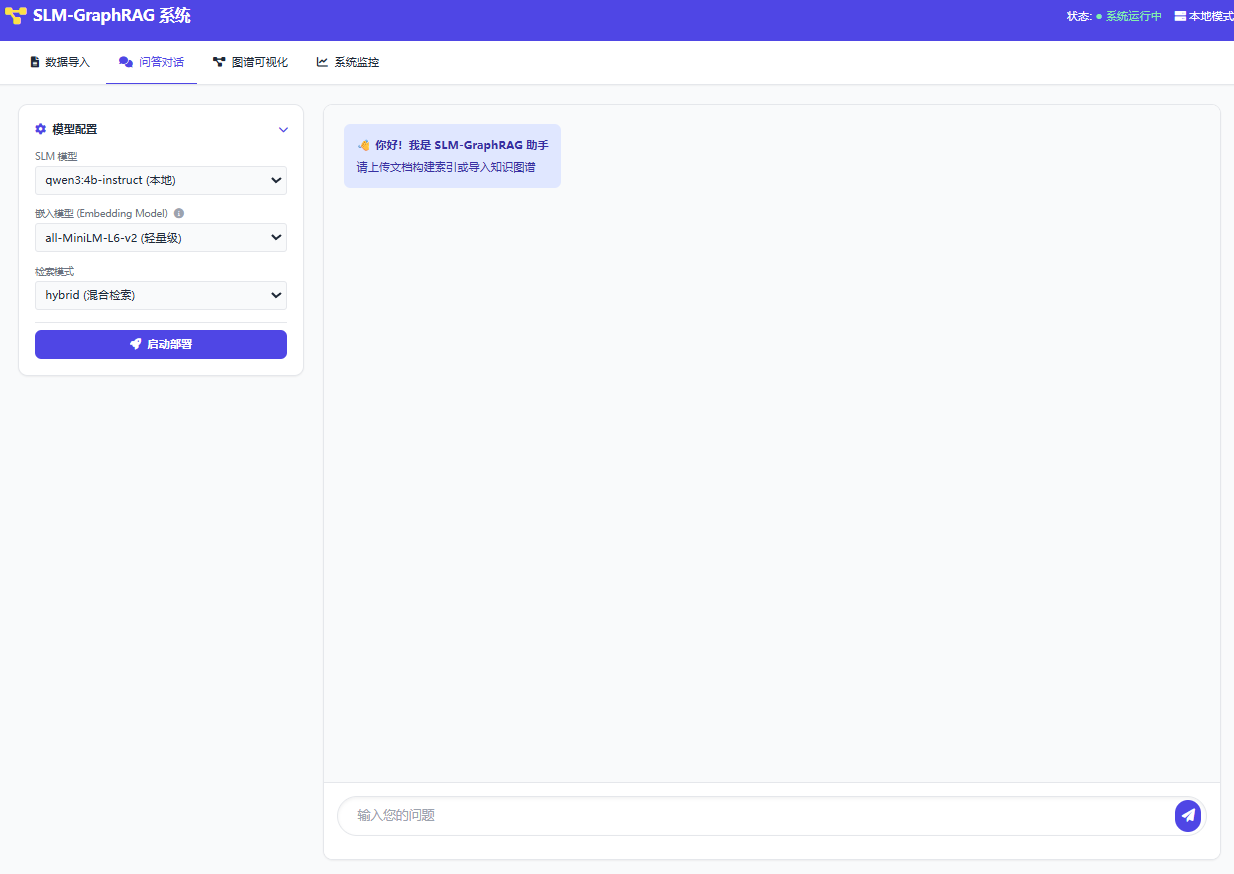
\includegraphics[width=\textwidth]{pic/5pic1.png}
\caption{系统主界面图}
    \label{fig:system_interface}
\end{figure}


\subsection{系统展示}

系统核心功能的实现效果主要通过以下五个功能模块进行展示:智能问答交互、图谱可视化、文档管理、实体管理与系统监控。

智能问答交互模块采用聊天式对话界面设计,支持用户以自然语言形式提交查询并实时获得结构化答案。界面划分为消息展示区与输入操作区两部分:消息展示区采用气泡式布局,区分用户查询与系统响应,系统响应中包含推理路径展示、引用来源标注以及性能指标统计(Token消耗、检索耗时、生成耗时等),使用户能够直观理解系统的推理过程并评估系统性能；输入操作区提供文本输入框与提交按钮,并实时显示当前查询的性能指标。

知识图谱可视化模块基于Cytoscape.js图形渲染库实现,支持知识图谱的交互式展示与探索。图谱可视化界面采用左右分栏布局,左侧为图谱控制面板,右侧为图谱画布。控制面板提供节点搜索、重新布局、图谱导出等核心功能,以及图统计信息(节点数、边数)的实时展示。图谱画布支持缩放、平移、拖拽等交互操作,节点按实体类型采用不同颜色标识。用户可通过节点搜索快速定位目标实体,点击节点可查看实体详情,包括实体描述、关联关系、属性信息及来源文档,使用户能够直观探索实体间的语义关联。图\ref{fig:visualize}展示了知识图谱可视化模块的界面布局。

\begin{figure}[htb]
    \centering
    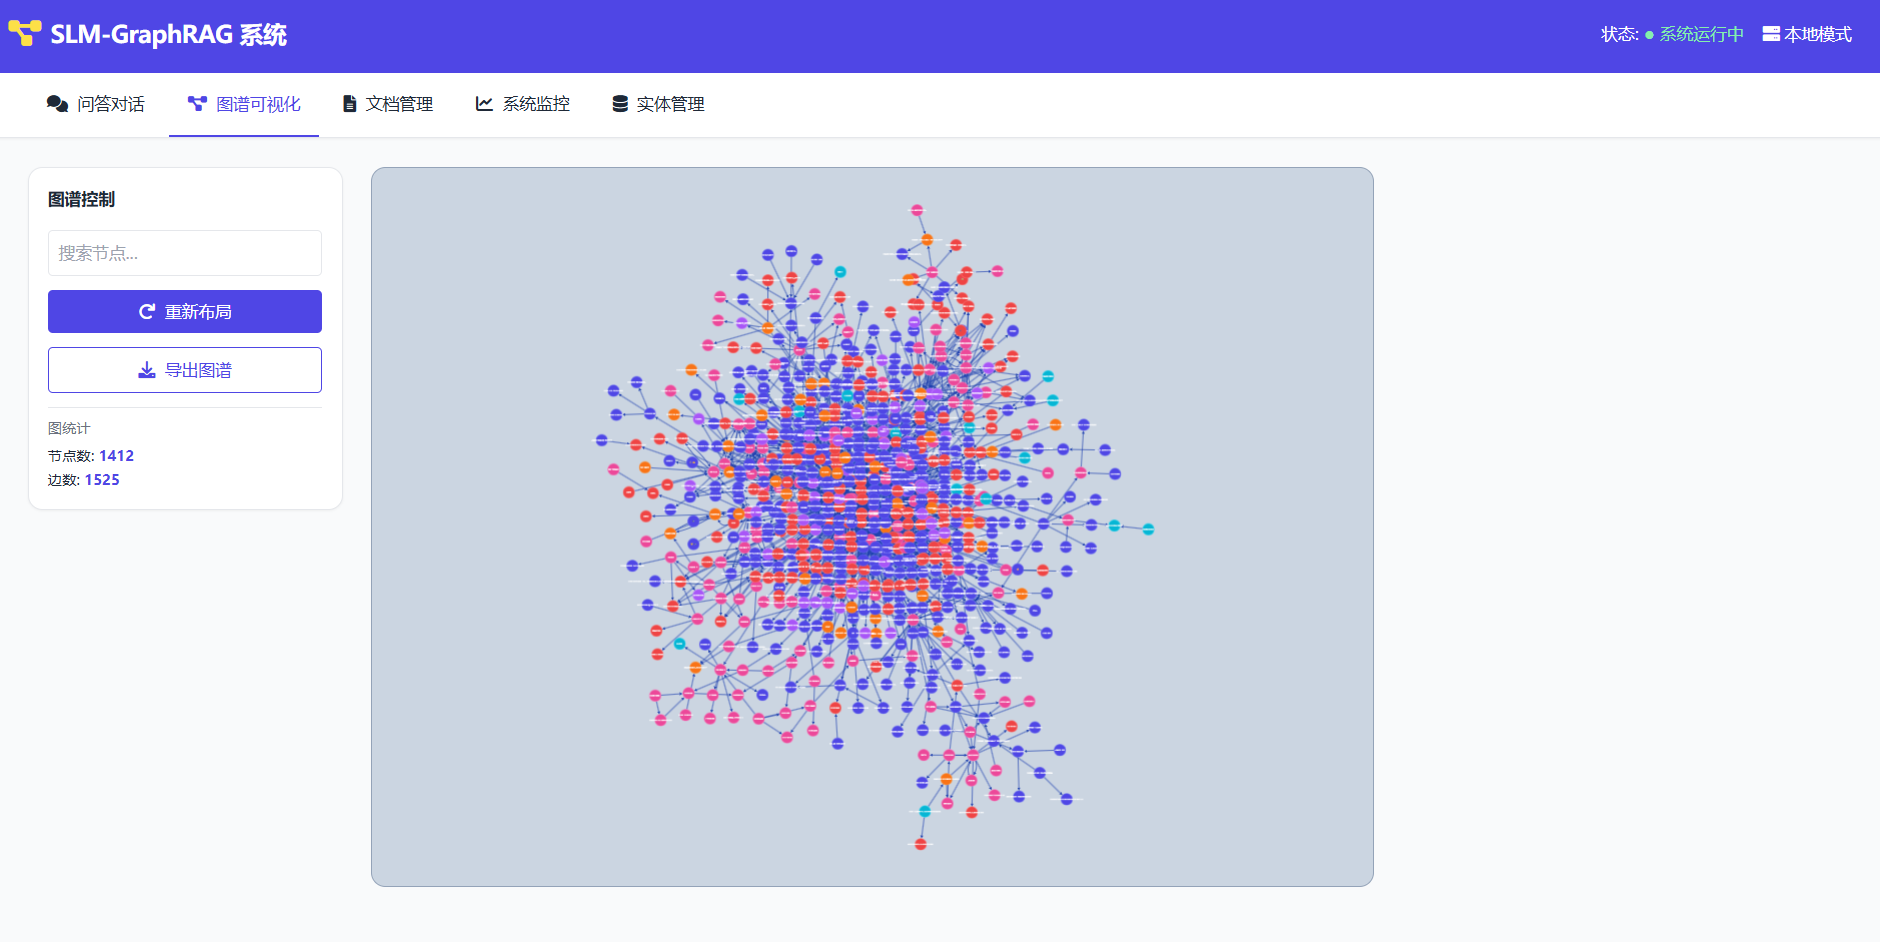
\includegraphics[width=\textwidth]{pic/5pic_visual.png}
\caption{知识图谱可视化界面图}
    \label{fig:visualize}
\end{figure}

文档管理模块提供文档列表视图,采用表格形式展示文件名、大小、上传时间、处理状态及索引统计等信息。该模块支持文档上传、删除与刷新操作,处理状态分为待处理、处理中、已完成与失败四种类型,索引统计包含文本块数量、实体数量与关系数量。表格顶部提供快速操作按钮,用户可通过该模块监控文档处理进度,确保知识库构建的完整性。图\ref{fig:5picfile}展示了文档管理模块的界面布局。

\begin{figure}[htb]
    \centering
    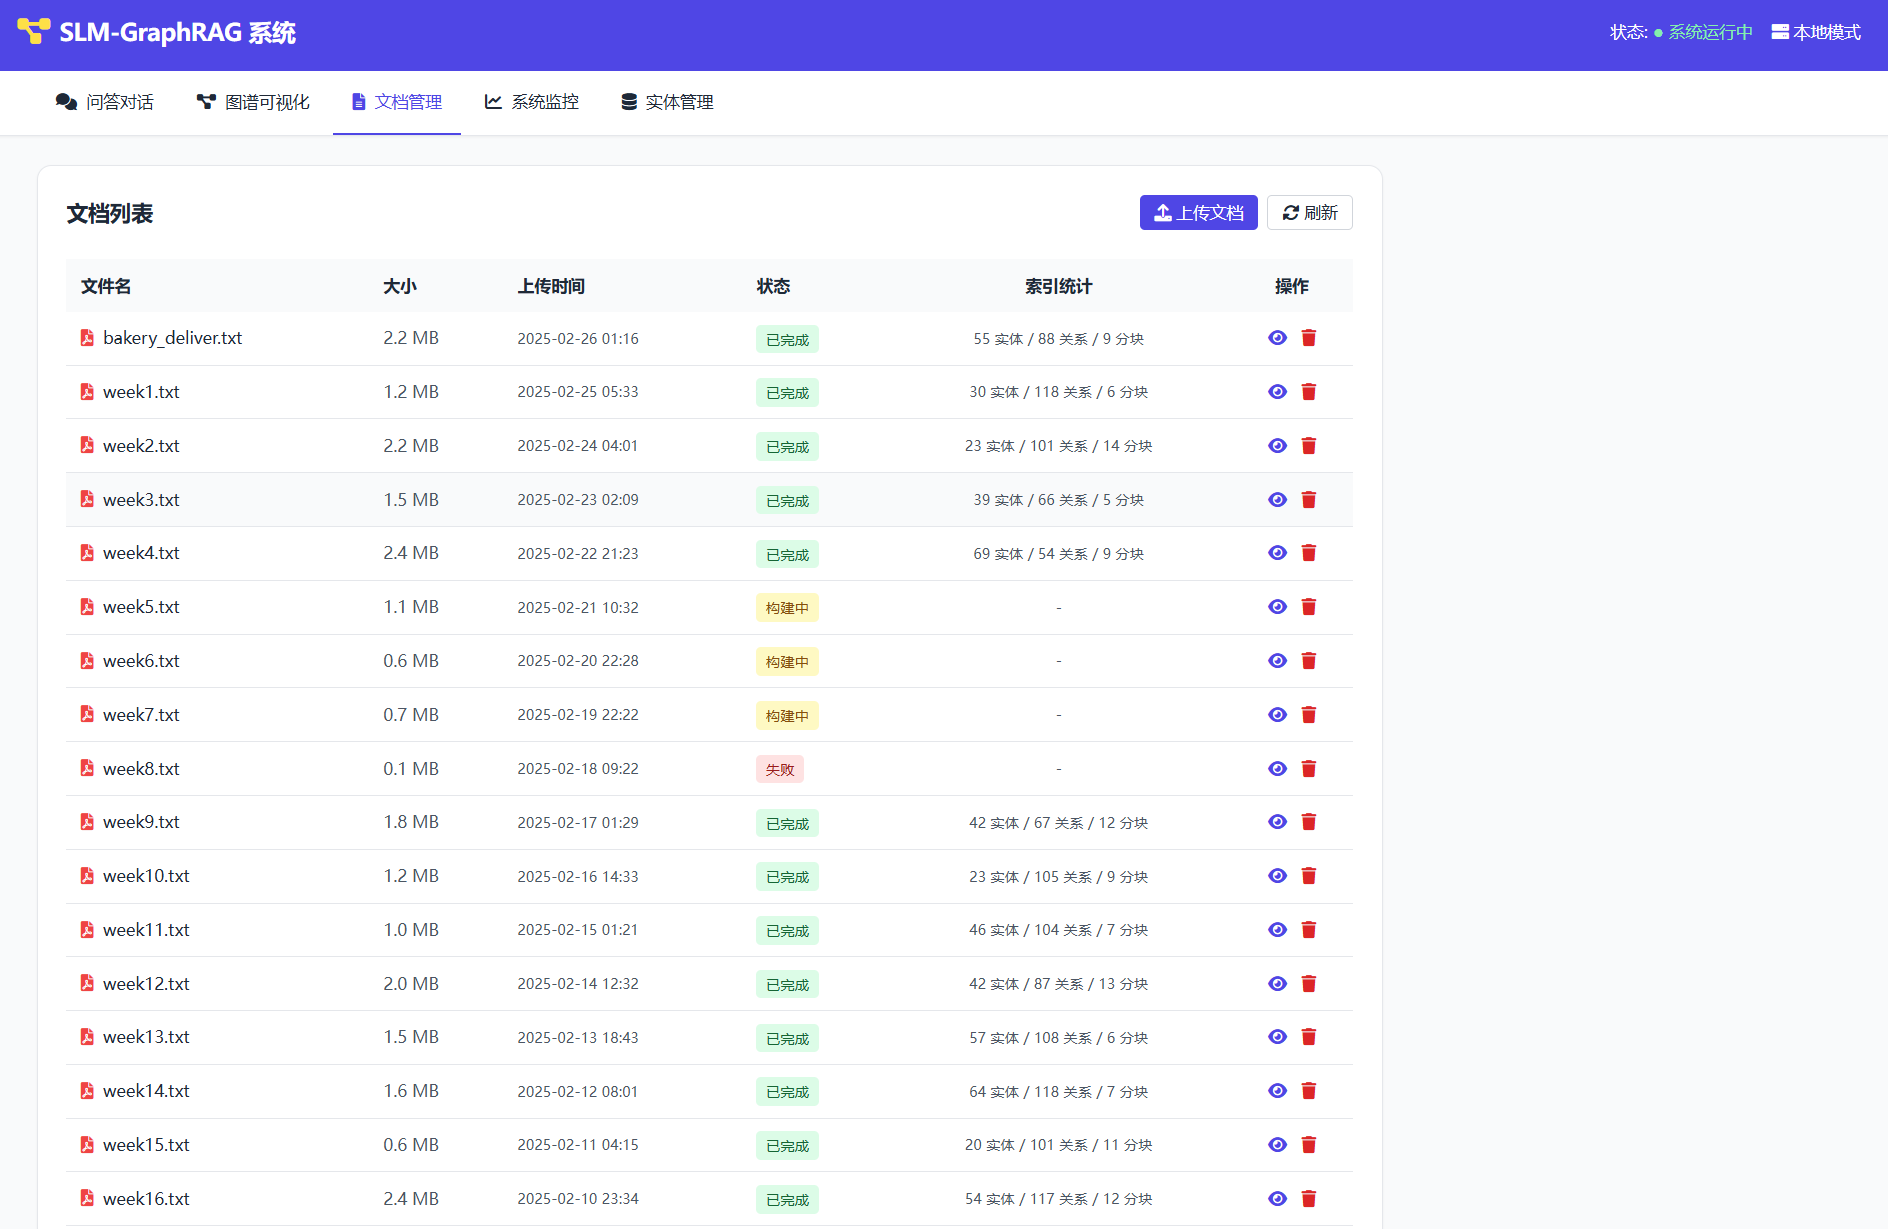
\includegraphics[width=\textwidth]{pic/5pic_file.png}
\caption{文档管理界面图}
    \label{fig:5picfile}
\end{figure}

实体管理模块采用左右分栏布局,左侧为实体搜索与列表区,右侧为实体详情展示区。搜索区支持关键词模糊搜索与按实体类型筛选(人物、组织、地点、概念等),实体列表采用滚动视图展示匹配结果。详情区展示选中实体的完整信息,包括实体描述、关联关系、属性信息,帮助用户深入了解实体的语义内容与上下文关联。图\ref{fig:5entity}展示了实体管理模块的界面布局。

\begin{figure}[htb]
    \centering
    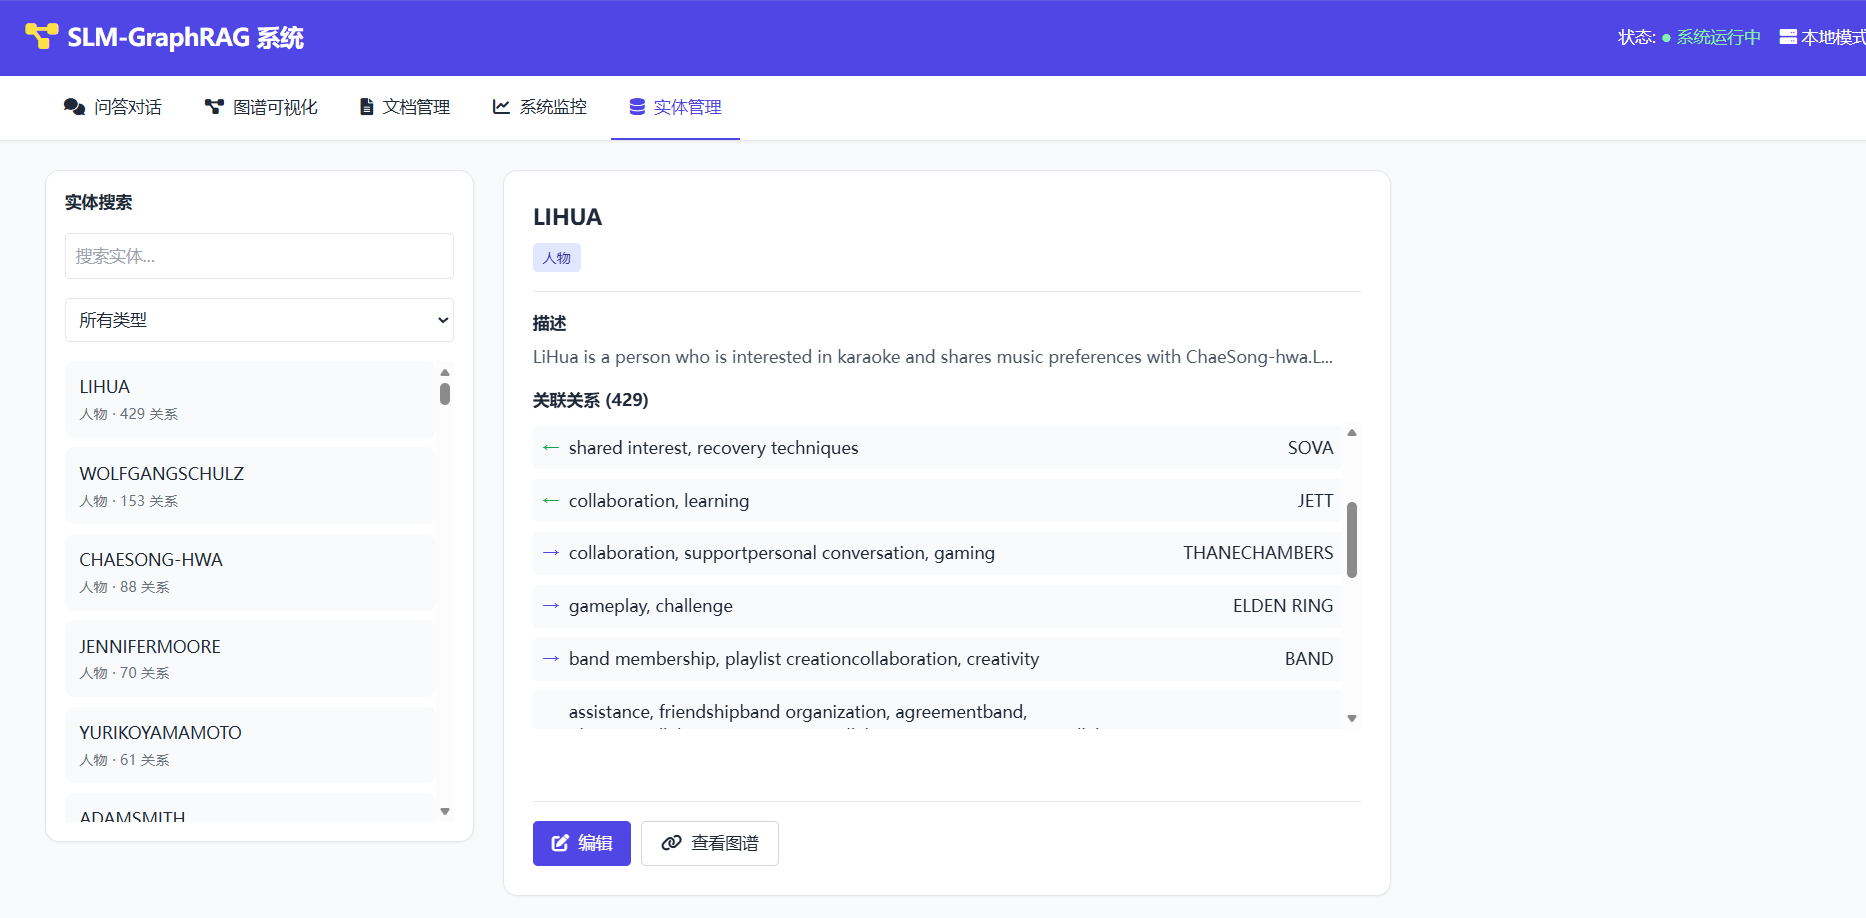
\includegraphics[width=\textwidth]{pic/5pic_entity.png}
\caption{实体管理界面图}
    \label{fig:5entity}
\end{figure}

系统监控模块通过顶部状态信息、核心指标卡片与系统日志三个维度展示系统运行状态。页面顶部显示系统运行状态与部署模式,帮助用户快速确认当前环境；核心指标卡片集中展示图谱规模、累计查询数以及内存与显存占用等关键指标；系统日志区域采用终端风格展示索引构建、图写入与初始化等关键操作信息,按时间顺序记录时间戳、日志级别与具体内容,为系统运维与问题排查提供数据支撑。
图\ref{fig:5watch}展示了系统监控模块的界面布局。

\begin{figure}[htb]
    \centering
    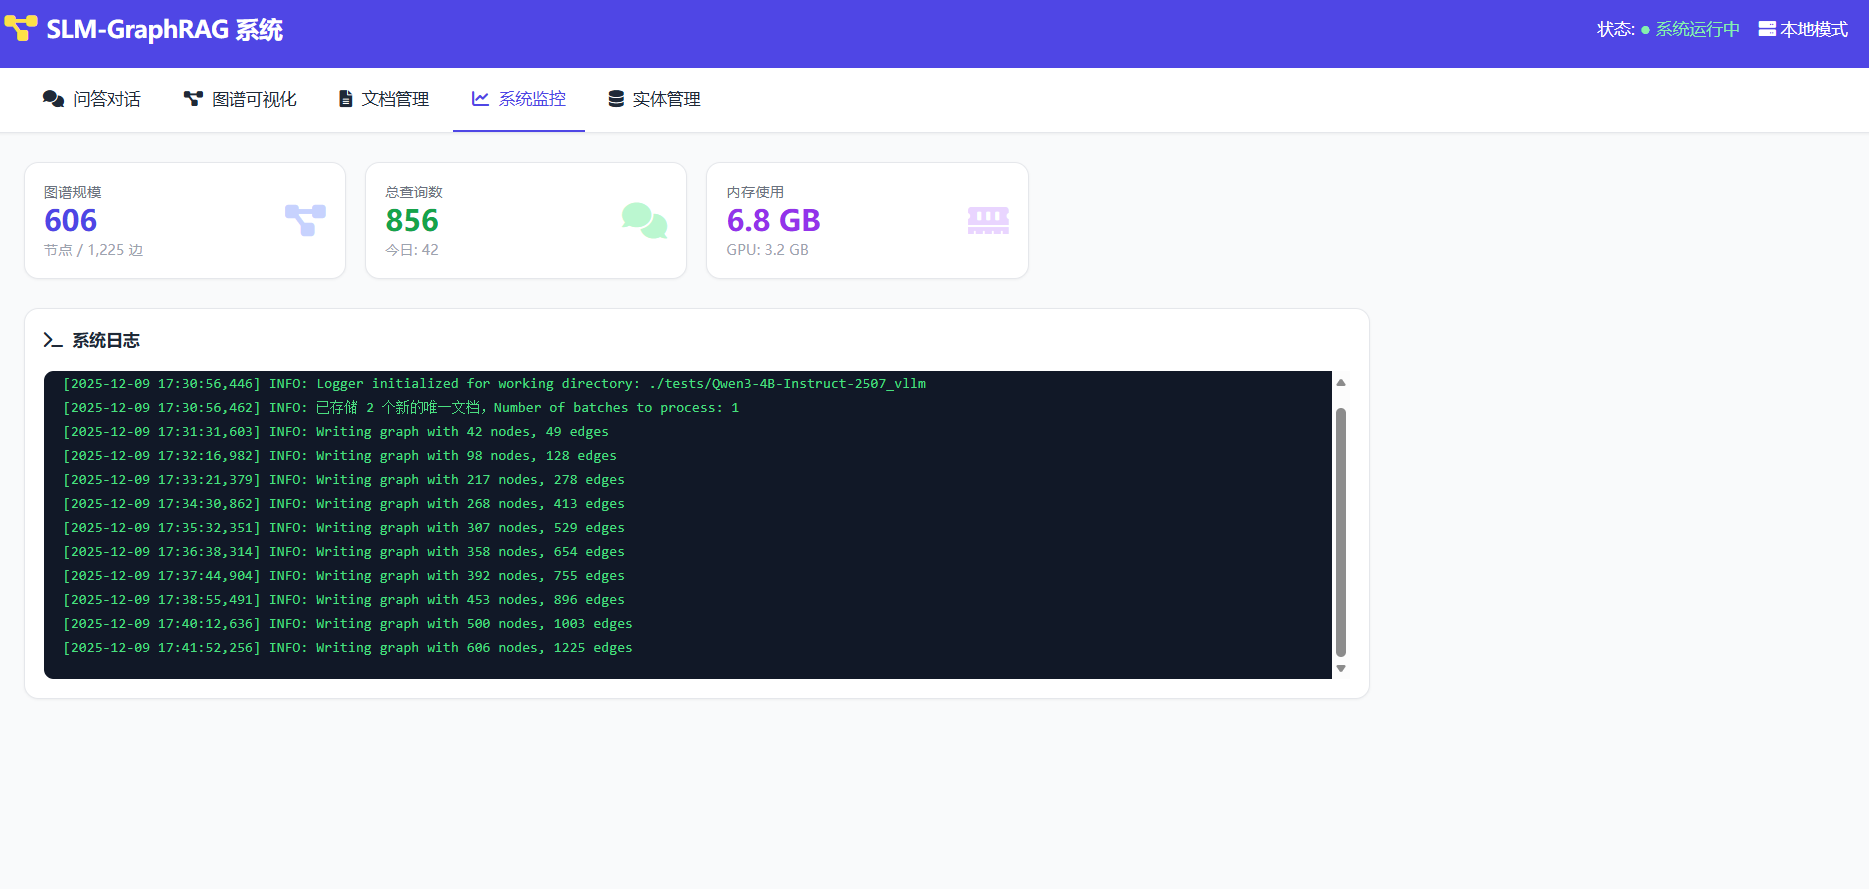
\includegraphics[width=\textwidth]{pic/5pic_watch.png}
\caption{系统监控界面图}
    \label{fig:5watch}
\end{figure}


\subsection{系统应用}

SLM-GraphRAG系统作为面向本地私有化部署的图基检索增强生成系统,具有隐私保护、本地化部署、多跳推理能力等核心优势,可广泛应用于以下场景:

(1)企业知识管理。企业内部积累了大量技术文档、产品手册、会议纪要、项目报告等非结构化知识资产,传统关键词检索难以满足跨文档关联推理需求。SLM-GraphRAG系统可将企业文档转化为结构化知识图谱,支持员工通过自然语言查询获取跨文档的关联知识,例如“某产品在哪些项目中被使用过”、“某技术方案的演进历史”等复杂问题,显著提升企业知识资产的利用效率。

(2)个人知识助手。个人在长期学习与工作中积累了大量笔记、文章、电子书等知识资源,这些资源往往分散存储且缺乏有效关联。系统可帮助用户构建个人知识图谱,支持基于语义的智能检索与知识关联探索,例如“我在哪些文档中提到过某个概念”、“某主题的知识在我笔记中的演变过程”等查询,实现个人知识的结构化管理与智能复用。


\section{系统测试}

在完成面向小型语言模型的图基检索增强生成系统的设计与开发后,为了验证系统是否满足设计需求,本文对系统的功能需求与非功能需求进行了测试。测试内容涵盖了系统测试环境的介绍,以及设计了功能测试和性能测试。本测试旨在确保系统的稳定性和可靠性。

(1)系统环境

在进行系统测试之前,对测试环境进行了详细的配置和记录。系统在开发和测试过程中使用了多种硬件和软件环境。为了确保系统的高效性和稳定性,本系统选用了高性能的本地工作站,并配置了合适的软件开发工具及框架。系统环境的具体配置如表\ref{tab:env_config}所示。

\begin{table}[htb]
\caption{系统环境配置表}
\centering
\begin{tabular}{cc}
\toprule
系统环境 & 规格 \\
\midrule
操作系统 & Ubuntu 24.04.3 \\
处理器 & Intel(R) Core(TM) i5-14600KF \\
内存 & 16GB \\
编程语言 & Python 3.12 \\
语言模型 & Qwen3-4B-Instruct \\
最长上下文长度 & 8192 \\
推理框架 & vLLM \\
嵌入模型 & all-MiniLM-L6-v2 \\
图数据库 & NetworkX \\
向量数据库 & NanoVectorDB \\
文档数据库 & JSON文件存储 \\
前端框架 & JavaScript \\
\bottomrule
\end{tabular}
\label{tab:env_config}
\end{table}

(2)功能测试

功能测试旨在验证系统是否能够满足用户的基本操作需求,确保各个功能模块均能够正常运行并满足用户需求。测试采用LiHua-World数据集的部分数据作为测试基准,该数据集包含442篇聊天记录文档。功能测试结果如表\ref{tab:core_function_test}所示,系统的各个功能模块均能够正常运行并满足用户需求。智能问答交互功能稳定可靠,能够正确返回结构化答案并展示推理路径与引用来源。知识图谱可视化功能能够正确渲染实体节点与关系边,支持交互式探索。文档管理与实体管理功能能够准确展示处理状态与实体信息,系统监控功能能够实时反映系统运行状态,便于用户了解系统运行情况与决策。

\begin{table}[htb]
\caption{功能测试用例及结果}
\centering
\setlength{\tabcolsep}{3pt}
\begin{tabular}{@{}>{\raggedright\arraybackslash}p{1.5cm}>{\raggedright\arraybackslash}p{2.7cm}>{\raggedright\arraybackslash}p{2.9cm}>{\raggedright\arraybackslash}p{3.8cm}>{\centering\arraybackslash}p{1.1cm}@{}}
\toprule
测试功能 & 测试内容描述 & 预期结果 & 实际结果 & 测试状态 \\
\midrule
智能问答交互 & 验证用户能否以自然语言提问并实时获得结构化答案,界面能否展示推理路径、引用来源及性能指标 & 系统正确返回答案,推理路径与引用来源标注完整,性能指标实时显示 & 637组查询均正常返回结果,推理路径与来源标注正确,Token消耗与耗时统计正常展示 & 通过 \\
知识图谱可视化 & 验证图谱可视化界面是否能正确渲染实体节点与关系边,支持搜索、缩放、拖拽与实体详情查看 & 可视化界面正确展示节点与边的拓扑结构,节点搜索与详情查看功能正常 & 图谱正确渲染实体与关系,节点搜索、详情查看与图谱导出功能均正常 & 通过 \\
文档管理 & 验证文档上传、删除与刷新功能是否正常,处理状态及索引统计信息是否正确展示 & 文档列表正确显示文件名、大小、处理状态及索引统计,上传与删除操作正确执行 & 442篇文档成功处理,状态从待处理转为已完成,文本块、实体与关系数量统计显示正确 & 通过 \\
实体管理 & 验证实体关键词搜索、按类型筛选及实体详情展示功能是否正常工作 & 搜索与筛选结果准确,实体描述、关联关系与来源文档展示完整 & 关键词搜索与类型筛选结果准确,实体详情面板正确展示描述、属性与关联关系 & 通过 \\
系统监控 & 验证状态信息、核心指标卡片与系统日志是否能正确反映系统运行状态 & 图谱规模、累计查询数、内存显存占用及系统状态正确展示,日志记录关键操作 & 顶部状态信息显示正常,各指标卡片数据正确刷新,日志按时间顺序记录索引构建与图写入等操作 & 通过 \\
\bottomrule
\end{tabular}
\label{tab:core_function_test}
\end{table}

(3)性能测试

性能测试主要评估系统在高负载条件下的响应速度以及数据处理能力关键性能指标。性能测试结果如表\ref{tab:performance_test}所示,系统在查询响应与资源占用控制方面表现良好。根据442篇文档的索引构建日志统计,平均每篇文档的索引构建时长约为304.43秒,满足320秒的预期指标。在查询响应方面,100个测试问题的平均响应时间为8.94秒,满足10秒的预期要求。在资源占用方面,系统峰值内存占用14.2GB,显存占用20.4GB,均在资源约束范围内,资源控制良好。综上所述,系统在交互响应、数据处理与资源管理方面能够满足本地私有化与资源受限单机场景下的基本负载需求。

需要进一步说明的是,本系统在第五章测试中采用 Qwen3-4B-Instruct 作为生成模型,并通过 vLLM 框架进行本地推理。对于 4B 级模型而言,在 8k 上下文长度配置下,4090(24GB) 上出现约 20GB 的显存占用属于正常现象。
首先,模型权重本身构成稳定的静态开销。以 FP16 精度加载 4B 参数模型时,理论权重占用约为 $4\times10^9 \times 2 \text{ Byte}\approx 8$GB。
其次,vLLM 为提升吞吐效率,会根据最大上下文长度与并发请求规模预分配 KV cache blocks;
与此同时,vLLM 默认采用较高的 GPU memory utilization 比例,会对可用显存进行较激进的预留与分配,进一步放大显存接近满载的现象。

综合来看,在本文测试配置下,约 8GB 的模型权重、8--12GB 的 KV 缓存以及 3--5GB 的中间状态与系统开销共同叠加,最终形成约 20GB 的总显存占用。
因此,表\ref{tab:performance_test}中观测到的 20.4GB 峰值显存并不意味着系统存在异常的资源浪费,而是 vLLM 在长上下文推理场景下为保证吞吐与稳定性所呈现出的典型运行特征。

对于显存更为受限的本地设备,可以进一步采用两类资源压缩策略:一是优先选择量化版本模型,以 AWQ、GPTQ 或 INT8 等低比特量化模型替代 FP16 精度模型,从而显著降低模型权重的静态显存占用;
二是在 vLLM 部署时适当下调 GPU memory utilization 等参数,主动压缩 KV cache 的预留空间与并发容量,以换取更低的峰值显存消耗。
上述策略虽然可能在一定程度上影响吞吐率或生成质量上界,但对于资源受限单机环境而言,能够有效提升系统的可部署性与运行稳定性。

\begin{table}[htb]
\caption{性能测试用例及结果}
\centering
\setlength{\tabcolsep}{3pt}
\begin{tabular}{@{}>{\raggedright\arraybackslash}p{1.6cm}>{\raggedright\arraybackslash}p{2.8cm}>{\raggedright\arraybackslash}p{2.8cm}>{\raggedright\arraybackslash}p{3.2cm}>{\centering\arraybackslash}p{1.2cm}@{}}
\toprule
测试指标 & 测试场景 & 预期结果 & 实际结果 & 测试状态 \\
\midrule
数据处理时间 & 上传442个测试文档 & 平均处理时长$\leq$320秒 & 按日志统计平均每篇文档处理时长为304.43秒 & 通过 \\
查询响应时间 & 对100个测试问题进行查询 & 平均响应时间$\leq$10秒 & 平均响应时间为8.94秒 & 通过 \\
资源占用 & 系统运行期间的内存占用与显存占用 & 内存占用$\leq$16GB,显存占用$\leq$24GB & 峰值内存占用14.2GB,显存占用20.4GB & 通过 \\
\bottomrule
\end{tabular}
\label{tab:performance_test}
\end{table}


\section{本章小结}

本章围绕面向小型语言模型的图基检索增强生成系统的设计与实现展开,全面介绍了系统的需求分析、功能设计、数据库设计以及系统展示等内容。
在系统需求分析部分,明确了系统的功能需求与非功能需求,确保系统能够满足用户对智能知识管理与问答服务的需要。
在系统测试部分,通过功能测试验证了系统在智能问答交互、知识图谱可视化、文档管理、实体管理与系统监控等五大功能模块上的正确性与完整性;通过性能测试验证了系统在数据处理时间、查询响应时间与资源占用控制等方面满足本地私有化与资源受限单机部署场景的需求。测试结果表明,系统各项功能运行正常,具备实际应用场景下的使用基础。





\chapter{全文总结与展望}

\section{全文总结}

随着大语言模型技术的快速发展,检索增强生成已成为提升模型知识覆盖度和事实准确性的关键技术。然而,现有图基检索增强生成系统高度依赖大型语言模型,面临着计算成本高昂、隐私数据安全风险以及边缘设备适配困难等挑战。小型语言模型在参数规模、部署效率和隐私保护方面具有显著优势,但在图索引构建与检索增强生成任务中仍面临指令遵循能力弱、幻觉严重、长上下文处理效率受限等核心瓶颈。本文针对上述问题,从图索引构建与检索方法两个维度展开研究,提出了一套完整的面向小型语言模型的图基检索增强生成优化方案。本文的主要研究工作如下：

(1)提出了验证优先图索引构建方法(VF-GIM)
针对小型语言模型在实体关系抽取阶段存在的指令遵循能力弱、幻觉严重和共指消解不足等问题,本文提出了验证优先图索引构建方法。该方法包含基于验证优先策略的VF-ERE模块和轻量化的图数据去重合并模块。VF-ERE模块利用认知非对称性原理,设计了“先验证、后修正”的迭代式抽取机制,通过反向推理与正向补全相结合的策略缓解模型的“自我中心偏差”问题。轻量化去重合并模块包含启发式实体去重机制、多数投票类型决策机制和分治描述迭代摘要机制,改善图索引的纯净度与一致性。实验结果表明,在当前实验设定下,VF-GIM方法在实体召回率、关系召回率和幻觉控制等指标上相较GraphRAG和MiniRAG等基线方法表现更优。

(2)提出了查询语义引导的边感知增强检索方法(Semantic-Flow RAG)

针对图基RAG在检索阶段存在的起点定位偏差与冗余路径噪声问题,本文提出了查询语义引导的边感知增强检索方法。该方法设计了融合实体名称向量索引与实体语义向量索引的两阶段候选召回机制,实现从查询语义到图节点的较高精度映射；提出了融合边语义权重的自适应流式剪枝算法,依据边的语义描述与查询的相关性动态筛选高价值推理路径；设计了按路径可靠性升序的结构化提示增强机制,将较关键的推理路径置于上下文末端。实验结果表明,在本文统一的小模型与统一预算约束设定下,Semantic-Flow RAG方法相较所选基线取得了更高的问答准确率与更稳定的整体表现。

(3)设计并实现了SLM-GraphRAG系统

在上述两项方法的基础上,本文设计并实现了面向小型语言模型的图检索增强生成系统。系统采用分层模块化架构,涵盖数据层、处理层、检索层与应用层,支持本地化全流程部署。系统集成了VF-GIM与Semantic-Flow RAG两套核心算法,提供了图谱可视化、文档管理、实体管理与系统监控等完整的Web界面功能。通过功能测试、性能测试、算法消融实验与稳定性测试对系统进行了评估,结果表明该系统在本地私有化SLM场景下具有一定有效性与实用价值。

\section{后续工作展望}

本文在面向小型语言模型的图基检索增强生成领域取得了一定的研究成果,但仍存在一些局限性与改进空间。未来的研究工作可以从以下几个方向展开：

(1)多模态图索引构建。本文的研究主要聚焦于纯文本场景下的图索引构建与检索。然而,在实际应用中,知识往往以多模态形式存在,包含文本、图像、音频、视频等多种数据类型。未来的工作可以探索如何将多模态信息整合到图索引中,构建跨模态的实体关系网络,为检索增强生成系统提供更丰富的语义信息,进一步提升系统在复杂场景下的表现。

(2)动态图谱更新机制。本文所提出的图索引构建方法主要针对静态文档集合。然而,在现实应用中,知识是动态变化的,新信息不断涌现,旧信息可能过时或失效。未来的研究需要探索如何设计高效的动态图谱更新机制,实现图索引的增量更新与演化,使RAG系统能够适应知识快速变化的应用场景,如新闻资讯、社交媒体等。

综上所述,面向小型语言模型的图基检索增强生成研究仍有广阔的发展空间。未来的研究工作可以在多模态融合、动态更新等多个方向持续深化,推动图基RAG技术在更广泛的应用场景中落地生根,为构建低成本、高隐私、智能化的下一代知识服务系统提供有力支撑。

\bibliography{ref}

\end{document}
